\documentclass[../main.tex]{subfiles}
\begin{document}
\begingroup
% Paper-specific macros for the Internal Tide-Eddy chapter and its appendix.
% Always \input inside a \begingroup..\endgroup so they cannot leak into other
% chapters' math, since several of these names are also used with different
% meanings elsewhere, e.g. \grad, \div, \hat, \bar.
% Macros the chapter never called were removed; the original paper keeps them.
\renewcommand{\hat}{\widehat}
\newcommand{\p}{\partial}
\newcommand{\bs}[1]{\boldsymbol{#1}}
\renewcommand{\del}{\nabla}
\newcommand{\bsh}[1]{\boldsymbol{\hat{#1}}}
\newcommand{\dd}[2]{\frac{d{#1}}{d{#2}}}
\renewcommand{\bar}[1]{\overline{#1}}
\renewcommand{\t}[1]{\widetilde{#1}}
\renewcommand{\grad}[1]{\del#1}
\renewcommand{\div}[1]{\del . {#1}}


\chapter{Internal Tide-Eddy Interactions and the Formation of Internal Wave Continuum}\label{tide-eddy}

% \noindent\textit{C. Rajarshi$^{a}$ and Jim Thomas$^{a,b}$}\\
% \noindent\textit{$^{a}$International Centre for Theoretical Sciences, Tata Institute of Fundamental Research, Bangalore 560089, India}\\
% \noindent\textit{$^{b}$Centre for Applicable Mathematics, Tata Institute of Fundamental Research, Bangalore 560065, India}

\begin{summary}
We investigate energetic interactions between internal tides with geostrophic flows at low, intermediate, and high Rossby numbers using  numerical simulations of the non-hydrostatic Boussinesq equations. Using a linear geostrophic-ageostrophic and slow-fast decomposition we explore the energy transfers between different turbulent flow components. We find  that the slow-fast decomposition does a good job at finding coherent large-scale eddies even at higher Rossby numbers, while the linear geostrophic-ageostrophic decomposition works well primarily at low Rossby numbers. The downscale energy cascade and dissipation of the fast flow component increases with increasing Rossby number, while the slow component cascades negligible energy downscale even at high Rossby numbers. At intermediate and high Rossby numbers the slow-fast interactions generate a broadband high-frequency continuum, with linear waves' contribution being slightly more than 50\% of the high frequency flow energy. On the other hand, low Rossby number flows' frequency spectra show only discrete peaks at tidal harmonics. Exploring the energy flux in physical space, we find that bulk of the net energy flux comes regions with low vorticity, divergence, and flux values. Our findings in general highlight the nature and variability of tide-eddy interactions across spatio-temporal scales.
\end{summary}


% \section*{Plain Language Summary}
% One-third of the net power put in the ocean comes from internal tides that form due to the gravitational pull of the Sun, the Moon, and other celestial objects. These internal tides control turbulent mixing throughout the ocean by exchanging energies with other internal waves, and slowly evolving balanced eddies. Such energy interactions at large scales differ considerably from those at small-scales. Due to computational limitations, small-scale interactions are poorly captured in current global ocean models. We investigate energy exchanges of internal tides with balanced flow across length scales. At large length scales, tide-eddy interactions are weak, with eddies transferring energy to large scales, hence preserving their coherent structures. At smaller length scales, tide-eddy interactions are stronger with more energy exchanged between the large-scale eddies and tides. Such interactions not only generate waves with harmonics of the tidal frequency, but also energize rapidly evolving non-wave motions. This leads to a broad spectrum of waves, known as an internal wave continuum, in the frequency spectra. Our study offers key insights on energy pathways for internal tides interacting with eddy flows across spatio-temporal scales in the ocean. %By quantifying pathways for tidal energy exchanges across length and timescales, our study offers new insights into small-scale turbulent mixing in the ocean. 
% \end{comment}

\section{Introduction}


The world's oceans cover about 70 percent of the Earth and store close to 90 percent of the energy gained by the Earth \citep{von2023}, significantly affecting the planet's climate and carbon cycle. Energy is transferred into the oceans through winds and barotropic tides that generate rapidly evolving internal gravity waves \citep{Garrett_Munk_1972, Munk_Wunsch_1998, FerrariWunsch09}. However, the bulk of the ocean's kinetic energy is contained within slowly evolving mesoscale eddies spanning across tens and hundreds of kilometers \citep{WF04, Chelton_etal_2007, FerrariWunsch09, Chelton11}. The interactions between the eddies and waves transfer energy across scales of thousands of kilometers down to a few meters, creating a global energy pathway. Understanding these interactions across scales is key to improving coarse-resolution climate-scale models, which lie at the heart of predicting the global climate behavior.

Winds blowing over the upper ocean generate near-inertial waves (NIWs) that evolve with the local Coriolis frequency, and control turbulent mixing and dissipation in the upper ocean \citep{pinkel1985, Alford_MacKinnon_Simmons_Nash_2016,whalen2018}. Internal tides (ITs), generated when tidal currents encounter the rough topography of the ocean floor \citep{GK07, vic2018, gao2024, kerry2013, ray1996}, propagate thousands of kilometers and their presence is  felt throughout the depth of the ocean \citep{rudnick2003, ray1996,zaron2022}. NIWs and ITs interact with other internal waves and eddies that drive turbulent energy mixing in the world's oceans.

Interactions of ITs with eddies are mostly studied at mesoscales, and they have various outcomes. Eddies can scatter and reflect ITs, generating incoherent waves \citep{Dunphy_Lamb_2014, PonteKlein15}. Tide-eddy interactions can generate high-mode internal waves \citep{Huang_etal_2018, Lob_etal_2020,fan2024}, and other non-wave motions that dissipate quickly \citep{wang2023}. These, in turn, control small-scale turbulent mixing. %Tide-eddy interactions can also significantly affect the eddies, by accelerating them \citep{shakespeare2023,fan2024}, or breaking them up \citep{Huang_etal_2018, Lob_etal_2020,fan2024}, contributing to both large and small scale energy transfers.
 %In this work, we investigate turbulent tide-eddy interactions for flows with different tidal and eddy energies at smaller submesoscales and compare them to the existing literature at mesoscales.

Nonlinear wave-wave and wave-eddy interactions can generate a high-frequency broadband spectrum, known as the internal wave continuum (IWC). Despite having some level of sensitiveness to the  regional dynamics, this broadband spectrum of waves is a universal feature repeatedly seen in a wide range of investigations   \citep{Garrett_Munk_1972, Polzin_Lvov_2011, Pollmann_2020, le2021}.  IWC is typically observed in regions of strong NIWs and  ITs \citep{Muller_etal_2015,le2021}. Numerical simulations of \cite{sugiyama2009} in two dimensions and coarse resolution results of \cite{Muller_etal_2015} in three dimensions further found that IWC only forms when both ITs and NIWs are strongly forced. Between NIWs and ITs, global observations of \cite{le2021}  indicate that IWC variations are strongly correlated with NIW energy, making NIWs the predominant controller of the IWC. Numerical simulations of \cite{delpech_etal_2024} also show a similar result. Lastly, resolving smaller scale submesoscale flows in numerical simulations further strengthens the IWC \citep{nelson2020}. Even in the absence of ITs, eddy-NIW interactions alone are seen to generate an IWC when small scales are sufficiently resolved \citep{Yang_etal_2023}. %Mesoscale studies find that dispersive waves dominate the IWC \citep{Ansong_etal_2024}. This may not carry over to submesoscales, and the broadband frequency spectrum may not arise solely from dispersive waves. Our study investigates this in detail.  


Contrary to the NIWs' case mentioned above, relatively less is known regarding the possibility of tidal interactions generating an internal wave continuum, especially in the absence of NIWs. Flows with strong ITs typically show a much steeper frequency spectra, with energy localized at the peaks of the tidal frequency and higher harmonics \citep{lin2020, Ansong_etal_2024, buijsman2025, rolland2025}. However, \citet{chen2019} demonstrated a special case:  ITs can interact with a rough topography and form an IWC. In these studies, the effect of energetic submesoscale flows on the tide's dynamics remains unaddressed.
Recent regional realistic simulations have started to examine internal tides interacting with mesoscale and submesoscale eddies. In this work we investigate such tide-eddy interactions across Rossby numbers in an idealized setting. % Our work provides a clean idealized Rossby-number parameter-based framework to understand such interactions.
 

At submesoscales of O($10$) km and below,   nonlinear interactions are stronger compared to mesoscale dynamics, and the flow Rossby number approaches  O$(1)$ values. Such flows behave very differently from mesoscale flows \citep{McWilliams_2016, Thomas_Tandon_Mahadevan_2008} and can significantly affect mesoscale flow energetics \citep{sasaki2017,su2018,klein2019}. Although submesoscale flows are crucial in transferring energy from the largest to the smallest scales in the ocean, ocean models often fail to capture them. As a result, ocean models that resolve low-mode tides and large-scale NIWs still do not resolve submesoscale flow dynamics accurately  \citep{Arbic_2022, Alford_MacKinnon_Simmons_Nash_2016}.

The limitations in ocean models resolving submesoscale dynamics have led to a variety of process-based studies exploring  NIW-eddy interactions in different configurations \citep{BWM17, TA20, TD20, Taylor_Straub_2020, TV22, delpech_etal_2024}. These studies have looked at wave-eddy interactions across different energy ratios for wave and eddy flows with varying Rossby numbers. The results from these studies have led to an improved understanding of flow energy transfers across spatio-temporal scales and between flow components in different dynamic regimes, forming a potential starting point for the construction of parameterizations for coarse resolution models. 


 To complement the work that has gone into exploring NIWs interacting with geostrophic flows in different dynamic regimes,  in this work, we undertake an investigation of internal tide-eddy interactions across different Rossby numbers and eddy-wave energy ratios. We explore energy transfers between wave and eddy fields and the broadening of the wave spectrum in these different dynamic regimes. We study flow dynamics using different flow decompositions and identify features of the turbulent flow cascades in varying dynamic regimes. 

The manuscript is planned as follows:  \S \ref{edwv-dets} describes the governing equations and the flow decompositions we employ. \S \ref{edwv-ps} compares the physical structures in the different flow regimes, and \S \ref{edwv-cmp} contrasts the flow energetics across Rossby numbers. In \S \ref{edwv-fspectr}, we explore features of a broadband frequency spectrum in different regimes while  \S \ref{edwv-flux} investigates the turbulent cascade efficiency of these flows. Finally, we summarize our findings in \S \ref{edwv-sum} and discuss their implications.


 


% for multiple reasons. Firstly, directly computing turbulent flows spanning across length scales of mesoscales and submesoscales remains computationally infeasible. The alternative approach of deriving reduced order models for submesoscale flows is also challenging as the Rossby number is O$(1)$. Parameterizing these flows dynamics is also nontrivial   due to the non-universality and seasonality of submesoscale flow interactions, which can transfer energy both to large and small scales \citep{schubert2020, jing2021, zhang2021,balwada2022}, and their strength varies across seasons \citep{Callies_Ferrari_Klymak_Gula_2015, Brannigan_etal_2015, Buckingham_etal_2016, Qiu_etal_2014, berta2020,cao2023}.

%Submesoscale observations require fine-scale data, which is easier to obtain in the upper ocean where NIWs dominate. Consequently, the bulk of the submesoscale observations focus on upper ocean \citep{Thompson_etal_2016, QNCK17,berta2020}, and the numerical studies explaining them neglect the ITs \citep{Yu_etal_2019, Yang_etal_2023, srinivasan_etal_2023, solodoch2023}. Eddy-NIW interactions in such flows generate small-scale structures and fronts that are regions of strong energy transfers. Multiple observations suggest submesoscale flows to be considerably strong well below the mixed layer \citep{Erickson_etal_2020, zhang2021}, where they could interact with internal tides. Hydrostatic MITgcm simulations of \cite{Siegelman_2020} show a similar result.
 
%Two studies of submesoscale dynamics are of importance. In their study of the upper ocean, which focuses on NIW-eddy interactions, \cite{delpech_etal_2024} investigated submesoscale dynamics with the CROCO model that uses the hydrostatic Boussinesq equation on an $f$-plane. In passing, they compared ITs and NIWs, mentioning that the latter is more potent at forming the IWC. Recently, using the Modular Ocean Model (MOM6), \citet{wang2025} investigated horizontal and vertical energy transfers in the Western Atlantic, and reported high Rossby number flows with significant tide-eddy interactions, especially during winter.

%This study contrasts tide-eddy interactions across Rossby numbers and asks whether they are sufficient to form an IWC. We consider flows with different tidal energies to also investigate how eddy-dominating flows are affected by tides across length scales.

% The world's oceans cover about 70 percent of the Earth and stores close to 90 percent of the energy gained by the Earth \cite{von2023}, acting as a prominent reservoir of energy and thereby affecting the planet's climate and carbon cycle. Due to the Earth's rotation and stratification, a dominant share of the energy in the oceans move around the globe, trapped at mesoscales of the order of 50 km in the form of coherent eddies with a life span of the order of weeks to months \citep{WF04, Chelton_etal_2007, FerrariWunsch09, Chelton11}. In contrast, the small scales of the order of meters and below, where the energy dissipates, do not feel the effect of the planet's rotation and stratification. They homogeneous isotropic turbulence, composed of turbulent vortical motions. Long-term predictions of the earth's weather and climate require a complete ocean's energy budget. Understanding the detailed aspects of the transition of the nature of oceanic flows from their largest scale to smaller ones is crucial for closing the oceanic energy budget, thereby helping us better predict longer range weather and climate of our planet.

% Energy is injected into the ocean through two of its primary sources, winds and tides \citep{Garrett_Munk_1972, Munk_Wunsch_1998, FerrariWunsch09}. Winds blow over the ocean, exciting near-inertial waves (NIWs) with frequency close to the inertial frequency, and these fast waves control turbulent mixing and dissipation in the upper ocean \citep{pinkel1985,alford2016,whalen2018}. The Sun, Moon, and other celestial bodies pull the water in the ocean, creating high tides that move around the globe. These surface or barotropic tides interact with the rough bottom topography in the oceans and generate baroclinic or internal tides with different vertical modes \citep{GK07, vic2018, gao2024, kerry2013, ray1996}. Bulk of the high vertical mode tides dissipate locally while low mode internal tides can propagate up to thousands of kilometers \citep{rudnick2003, ray1996,zaron2022}. During their propagation, low mode tides can interact with energetic eddy fields in the oceans and exchange energy. % Unlike the near-inertial waves (NIWs), generated from the near-inertial oscillations near the ocean surface, internal tides are not confined to the upper ocean. They distribute energy in the entire depth of the ocean. About $1$ TW, one-third of the net power put into the ocean, comes from internal tides \cite{Egbert_Ray_2003}. 

% %Regions with rough bottom topography like Sicily Channel \cite{gasparini2004,cosoli2015}, Mid-Atlantic Ridge \cite{bella2024,vic2018}, Hawaiian Ridge \cite{RP2006,Chavanne_etal_2010,zhao2011,ray1996}, Philippine Sea \cite{kerry2013}, South China Sea \cite{gao2024}, Bay of Bengal \cite{mohanty2018,jithin2019,peng2021}, and others \cite{klymak2016,tchilibou2020,niwa2001,RZ2016,Zhao_etal_2016} are sources of strong internal tides. Although some tidal energy is dissipated near its sources \cite{rudnick2003}, internal tides carry a significant amount of tidal energy hundreds of kilometers away from their sources \cite{ray1996,zaron2022}. This energy can go through multiple pathways before dissipating. 

% Internal tides interact with existing large mesoscale oceanic eddies in several ways. They can reflect and scatter off of geostrophic eddies. This changes the phases of the internal tides, and they become incoherent \citep{Dunphy_Lamb_2014, PonteKlein15, Savva_Vanneste_2018}. Internal tides also accelerate the eddies, transferring energy to larger length scales \citep{shakespeare2023,fan2024}. High energy low mode tides can also break up geostrophic eddies due to energy transfer from waves to geostrophic flow \cite{TY19}. Some low-mode internal tides interact with eddies and generate high-mode internal waves, thereby transferring energy to smaller scales \citep{Huang_etal_2018, Lob_etal_2020,fan2024}. Additionally, tide-eddy interactions also transfer energy to small-scale structures that dissipate quickly without generating any internal wave \cite{wang2023}. %In addition, internal tides also interact with other internal waves, generate small-scale flows, and cascade energy downscale, thereby increasing oceanic mixing \cite{rudnick2003, Suanda_etal_2018, Meyerjurgens_etal_2020, contreras2023}. Thus, in addition to the atmospheric and celestial forcing and viscous dissipation, flow components like internal tides and eddies can gain or lose significant energy through mutual interactions. This makes such interactions a crucial factor in quantifying the energy budget of the ocean.


% % Oceanic flows depend not only on the interactions in the bulk but also greatly on the boundary conditions. The boundary conditions across the ocean are extremely diverse, consequently making the flow vary across the globe. Data from observations and realistic oceanic simulations contain these boundary effects. Thus, they fail to capture the fundamental nature of energy exchanges among different flow components in the ocean. Idealized simulations in boxes centered around fixed latitude and longitude rid the complicated boundary conditions. Although they are bad at predicting realistic oceanic flows, they are useful in understanding the nature of energy transfers due to the flow components present everywhere in the global ocean. Studying the nature of the interaction between different flow components requires one to split the net flow into its components, eddies, and waves, for example. This is a challenging task in the ocean, which has an `ocean' of different kinds of flow. Data from the satellite and in situ observation are split either using spatial or temporal filters, assuming length and time scale separation of the different flow components. For idealised simulations, there are projection functions that can split the net flow into eddies and waves. Some of the decompositions are expensive but are more accurate, while others are easy to use but are prone to more errors. A systematic comparison between such decompositions is not yet established. 

% Nonlinear interactions between internal waves generate an internal wave continuum (IWC) in the frequency spectra of the flow variables. First pointed out by \citet{Garrett_Munk_1972}, and also referred to as the Garrett-Munk (GM) spectrum, this continuum has been an area of active oceanographic research for the past decades \citep{Fu_etal_1982, Lvov_Tabak_2001, Lvov_etal_2004,sugiyama2009, Polzin_Lvov_2011, Pan_etal_2020}. The IWC signifies the transfer of energy from low frequency large-scale waves to high frequency small-scale waves, where it is eventually dissipated. The GM spectrum has peaks at the NIW and tidal frequencies, with a close to $\omega^{-2}$ inertial range at higher frequencies. In observations, the slope of the continuum is seen to fluctuate around ${-2}$ across the global ocean \citep{Polzin_Lvov_2011, Pollmann_2020, le2021}. 

% % Eden_Pollmann_Olbers_2019

% Observations typically find an IWC in regions where both NIWs and internal tides are highly energetic \citep{Muller_etal_2015,le2021}. Consistent with this, numerical experiments using two-dimensional vertical plane model \cite{sugiyama2009}, and three-dimensional ocean models \cite{Muller_etal_2015} have found IWC to form when both NIWs and internal tides are strongly forced. Upon resolving smaller horizontal and vertical scales, \citet{nelson2020} found that small-scale submesoscale flows strengthens the IWC. In the absence of tides, \citet{Yang_etal_2023} showed that eddy-NIW interactions can generate an IWC, but only if sufficiently small horizontal scales are resolved. 

% Resolving only mesoscale flows in models typically generates a less energetic continuum which is considerably steeper than the GM spectrum. %However, regions of strong internal tides do not show an IWC in mesoscale-resolving studies. 
% The energy in the frequency spectra seen in such studies is localized at the tidal frequencies and their higher harmonics, with little energy in between \citep{lin2020, Ansong_etal_2024, buijsman2025, rolland2025}. In special cases, \citet{chen2019} showed that internal tides can interact with rough topography, generating new wave frequencies that lead to an IWC. In the context of the global ocean, \citet{le2021} investigated the correlation in the variability of the IWC with timescales of wind, tides, and mesoscale eddies. They found a significant correlation in the IWC variability with the NIW energy, thereby concluding that the global IWC is predominantly controlled by NIWs. \citet{delpech_etal_2024} also mentioned better potency of the NIWs in creating an IWC. However, the effect of tide-eddy interactions on the IWC at submesoscales is not clear, this forming a motivation for the present study. 

% % Observations from moorings show NIWs as the dominant contributor to the GM spectra in the upper ocean \cite{le2021}. Numerical simulations showed that NIWs interact with eddies at small scales and form the GM spectra \cite{Yang_etal_2023}. NIWs and tide interaction also lead to GM spectra, which is further enhanced by including smaller scales \cite{nelson2020}. Studies argue that tides alone cannot create an internal wave continuum \cite{Muller_etal_2015,sugiyama2009}. This is confirmed in mesoscale admitting ocean simulations and mooring observations, which show peaks of tidal harmonics in the frequency spectra \cite{Ansong_etal_2024,buijsman2025,rolland2025}. In the presence of rough topography, \citet{chen2019} showed that tides alone can create an internal wave continuum. This naturally poses the question whether internal tides and eddies can interact with each other at submesoscales to form the internal wave continuum.



% %Coherent eddies at scales of $\op{O}(100)$ km merge, grow in size, and accumulate energy. The Coriolis force due to the Earth's rotation dominates over the flow inertia at such large length scales. The outcome of internal wave-eddy interactions at these mesoscales depends on the relative strength of wave and eddy energy. In regions with strong wave energy, eddies are strengthened by the waves \cite{TY19}, whereas in regions of comparable eddy and wave energy, inertial waves dissipate the eddies \cite{Taylor_Straub_2020, Cusack_etal_2020}. 


% Globally, mesoscale tide-tide interactions dominate the frequency spectra, generating tidal harmonics \cite{buijsman2025}. This renders tide-eddy interactions at such scales weak. At intermediate submesoscales of 10 km and below, the flow inertia becomes comparable to that of the Coriolis force. Consequently, the nondimensional Rossby number, which captures the relative strength of flow inertia to the Coriolis force, becomes $\op{O}\left( 1 \right)$. The increase in the inertial forces increases nonlinear interactions, and the flow behavior differs from that of large mesoscale flows \cite{McWilliams_2016}. Although submesoscale flows have less energy than the mesoscale flows, they can significantly affect the mesoscale flow energetics, and are crucial in transferring energy from the largest scales to the smallest scales in the ocean \citep{sasaki2017,su2018,klein2019}. However, the dynamics of submesoscale flows are not often fully resolved in models due to multiple reasons. 

% First, capturing dynamics of such small scales together with the larger scales requires computational power inaccessible to current global ocean models. Second, the Rossby number of such flows can reach $O(1)$ values, which makes it challenging to derive reduced-order models that can be integrated faster. Third, numerical simulations and observations of submesoscale flows show that the energy transfer in these flows can be both upscale or downscale, which significantly alters the mesoscale flows \citep{schubert2020, jing2021, zhang2021,balwada2022}. This makes the flow interactions nonuniversal and difficult to parametrize in mesoscale-resolving models. Lastly, observations and a few numerical simulations show that submesoscale flow dynamics change seasonally, making a global understanding of such flows even more difficult \citep{Callies_Ferrari_Klymak_Gula_2015, Brannigan_etal_2015, Buckingham_etal_2016, Qiu_etal_2014, berta2020,cao2023}. As upper ocean observations are relatively easier than the deep ocean ones, a dominant share of submesoscale observational studies have focused primarily on the upper ocean \citep{Thompson_etal_2016, QNCK17,berta2020}. Since NIWs dominate the upper ocean internal waves, numerical studies aiming to explain upper ocean submesoscale dynamics have neglected internal tides \citep{Yu_etal_2019, Yang_etal_2023, srinivasan_etal_2023, solodoch2023}. They found that NIW-eddy interactions generate small-scale structures and fronts, and strengthen the IWC. 


% Compared to NIW-focussed studies, relatively fewer numerical studies have explored internal tide interactions with submesoscale flows. Notably, multiple observations have found submesoscale flows to be considerably strong in the ocean interior, well below the mixed layer \citep{Erickson_etal_2020, zhang2021}, and these could interact with internal tides. 
% % and NIWs are the dominant component of wave energy in the upper ocean, most studies have considered the behavior of NIWs with eddies in submesoscale admitting flows \cite{Thompson_etal_2016, QNCK17, Yu_etal_2019, Yang_etal_2023,cao2023,srinivasan_etal_2023,solodoch2023}. 
% Through hydrostatic simulations using MITgcm, \citet{Siegelman_2020} showed that in the presence of NIWs and internal tides, strong submesoscale flows persist well below the mixed layer. \citet{delpech_etal_2024} studied submesoscale flows using the CROCO model, which uses the hydrostatic Boussinesq equations on an f-plane. They commented on internal tides in passing, comparing them to NIWs and mentioning that NIWs are more potent at forming the IWC than internal tides. Recently, \citet{wang2025} investigated the interactions of internal tides with submesoscale eddies using the modular ocean model (MOM6), with an eye on differentiating horizontal and vertical energy transfer magnitudes. They found significant tide-eddy interactions in the Western Atlantic region, especially at higher Rossby numbers in winter. %They also found notable differences between vertical and horizontal energy transfers%The flow Rossby number in their study varied seasonally. From O(0.1) in the summer, it reached values around O(1) values during the winter. All the above-mentioned studies used realistic ocean models. Although the goal of such studies was to investigate the interactions between flow components, complicated boundaries of a particular region in the ocean can significantly affect such interactions. In fact, \citet{wang2025} mentions focusing specifically on regions where boundary effects are reduced to better capture the tide-eddy interactions.




% % At such scales, energy is transferred both upscale and downscale \cite{balwada2022, Deusebio_Vallgren_Lindborg_2013}. These intermediate scales, also known as submesoscales, link the energetics of the largest scales to the smallest ones. They significantly affect the energetics of large-scale flows \cite{Evans_etal_2020,sinha2023, Vladoiu_etal_2024,yu2024}. Therefore, understanding the flow dynamics and the nature of energy transfer at submesoscales has been the focus of significant oceanographic research \cite{Poje_etal_2017, Hernandez_etal_2021, Rossby_etal_2021, QNCK17, McWilliams_2016,cao2023, srinivasan_etal_2023,solodoch2023, Siegelman_2020, Siegelman_etal_2020, Thompson_etal_2016}. Properly capturing submesoscale flows in global ocean models remains impossible so far due to computational restrictions. Also, the Rossby number at these scales being $\op{O}(1)$ makes deriving reduced order models for these flows from primitive equations very difficult. Such high Rossby number flows also evolve faster, making flow interactions vary seasonally \cite{Callies_Ferrari_Klymak_Gula_2015, Brannigan_etal_2015, Buckingham_etal_2016, Qiu_etal_2014, Galperin_Sukoriansky_Qiu_2021}.
% % This makes understanding the fundamental nature of flow interactions challenging. The interactions between flow components like eddies and internal waves also change at submesoscales \cite{Cusack_etal_2020}. Observations and numerical simulations show that submesoscale flows show features like cyclone-anticyclone asymmetry in the ocean, something that is not captured by low Rossby number flows obeying QG equations \cite{Shcherbina_etal_2013, Lumpkin_Elipot_2010, Xu_Fu_2011}. Such flows also control turbulent and nutrient mixing in the mixed layer and the depth in the ocean \cite{Levy_Frank_Smith_2018,picard2024, Shcherbina_etal_2015, Erickson_etal_2020, Thompson_etal_2016, Yu_etal_2019}. While some studies have focused on the interaction of NIWs and eddies at submesoscales \cite{taylor2023}, the effects of internal tides at submesoscales are less understood. However, a quantitative understanding of the interactions across Rossby numbers and the strength of tidal energy and its outcomes is still.


% \rc{Several questions regarding tide-eddy interactions remain unanswered. Can tide-eddy interactions, without any near-inertial waves form an IWC at submesoscales? If so, then how does the submesoscale tide-tide and tide-eddy interactions differ compared to the mesoscales ones? What flow components make contribute to most of the energy interactions at different scales? In this chapter, we answer these questions using the non-hydrostatic Boussinesq equations in an idealized setting.}
% % In this work, we investigate turbulent baroclinic tide-eddy interactions across different Rossby numbers in an idealized setting using the non-hydrostatic Boussinesq equations. %Such idealized simulation replaces complicated boundaries with simple ones, and focuses solely on the nature of nonlinear interactions. 
% %To understand the dynamics of different flow components, we apply a slow-fast decompose the flow into its components using two separate flow decompositions. 
% \S \ref{edwv-dets} describes the governing equations, flow regimes, and the flow decomposition methods we employ. In \S \ref{edwv-ps}, we look at the physical structures of the flow and its decomposed components to qualitatively understand flow structures at different Rossby numbers. \S \ref{edwv-cmp} compares the nature of interactions of the different flow components and the spatial scales they dominate. In the following \S \ref{edwv-fspectr}, we explore the effects of the flow interactions in the frequency spectra. We also quantify the nature of the flows evolving faster than the inertial timescale. Finally, in \S \ref{edwv-flux}, we look at the strongly interacting regions of the flow using physical flux. We summarize our findings in \S \ref{edwv-sum} and discuss their implications.
% % \begin{itemize}
% % \item Among all, M$_2$ is the most dominant internal tide. 
% % \item Details of $Ro = 1$ flows, Krithin's paper. 
% % \item Is there any specific region of the turbulent flow that is associated with intense energy transfer? 
% % \end{itemize}


 

\section{Governing equations, flow decompositions, and numerical integrations} \label{edwv-dets}


We use the nondimensional Boussinesq equation on an $f$-plane given by
\begin{subequations}
 \label{edwv-bsnq}
 \begin{align}
 \Dp{\vec{v}}{t}{} + \hat{\vec{z}} \times \vec{v} + \del p + Ro \left( \vec{v}.\del + w\Dp{}{z}{}\right)\vec{v} &= \vec{F}_{\vec{v}}- \nu\Delta^{8} \vec{v}\\
 \Dp{w}{t}{} +\alpha^2 \left( \Dp{p}{z}{}-b\right) + Ro \left( \vec{v}.\del + w\Dp{}{z}{}\right) w &= F_w - \nu\Delta^{8} w\\
 \Dp{b}{t}{} + w + Ro \left( \vec{v}.\del + w\Dp{}{z}{}\right)b&= F_b -\nu\Delta^{8} b \\ 
 \del. \vec{v} + \Dp{w}{z}{} &= 0 \ ,
 \end{align}
\end{subequations}
where $\vec{v} = (u,v)$ is the horizontal velocity in the $x$ and $y$ directions respectively, $w$ is the vertical velocity in the $z$ direction, $b$ is the buoyancy, and $\nu$ is hyperviscosity multiplied with the eight power of the Laplacian operator $\Delta = \partial^2/\partial x^2 + \partial^2/\partial y^2 + \partial^2/\partial z^2$. $\del = \hat{\vec{x}}\partial/\partial x +\hat{\vec{y}} \partial/\partial y$ is the horizontal gradient operator. The `$F$' terms on the right-hand side of \eqref{edwv-bsnq} are forcing terms that inject energy into the flow. 


To arrive at the nondimensional equations \eqref{edwv-bsnq}, we used the inverse of the inertial frequency, $1/f$, to scale time, a length scale $L$ to scale horizontal coordinates, and a velocity scale $U$ to scale horizontal velocity components. A length scale $H$ was used to scale the vertical coordinate, and then the continuity equation led to the scale for vertical velocity as $UH/L$. Using geostrophic and hydrostatic balance conditions gave us the scales for pressure and buoyancy as $fUL$ and $fUL/H$, respectively. From these scalings, the Rossby number, $Ro=U/fL$, while $\alpha=N/f$ is the ratio of constant buoyancy frequency $N$ and inertial frequency $f$. Based on observations indicating the buoyancy frequency typically to be an order of magnitude or more than the inertial frequency \citep{Emery_etal_1984, Li_etal_2020}, we set $\alpha=20$. In \eqref{edwv-bsnq}, increasing   $Ro$ increases the nonlinear interaction strengths of the flow, indicative of the transition from mesoscales to submesoscales in the ocean. %In physical systems, the rotation rate $f$ around a particular latitude is fixed, and so is the typical speed $U$ of the oceanic flows. Changing Rossby number represents changing the length scales of the flow. 

In the absence of external forcing and viscous dissipation, \eqref{edwv-bsnq} conserves domain-integrated energy $E$ as 
\begin{equation}
    \label{edwv-en}
    \dd{E}{t}=0, \ E= \int_D \frac{1}{2} \left(  \bs v^2+  \frac{w^2}{\alpha^2} +  b^2 \right) dx dy dz ,
\end{equation}
where $D$ is a shorthand for the domain. 


%The flow has a total energy $E$ in the volume $V$, $E = \int dV \left( u^2 + v^2 + w^2/\alpha^2 + b^2 \right)/2$. 




\subsection{Flow decompositions} \label{edwv-dcmp}
To calculate interactions between tides and eddies, one needs to decompose the flow into  different  components.  In this work, we used two kinds of flow decompositions to separate flow components from the solutions generated by integrating \eqref{edwv-bsnq}. The two decompositions are the linear geostrophic-ageostrophic and the slow-fast, and these are described below. 


\subsubsection{Linear geostrophic-ageostrophic decomposition} \label{edwv-budcmp}

This decomposition splits the net flow into a geostrophic component, denoted by a subscript $g$ satisfying geostrophic and hydrostatic balance
% Setting the time derivatives and all the nonlinear terms multiplied by $Ro$ in \eqref{edwv-bsnq} to zero, and dropping forcing and dissipation, gives us 
\begin{equation}
    \label{edwv-gb}
    \bsh z \times \bs v_g + \del p_g =0, \ \p p_g/\p z-b_g=0, \ w_g=0, \ \del \cdot \bs v_g=0 \ ,
\end{equation}
and a remaining ageostrophic component $\vec{v}_{a} = \vec{v} - \vec{v}_g, ~w_{a} = w - w_g = w,~ b_{a} = b - b_g $. Used commonly in the literature \citep{Bartello95, Embid_Majda_1998, Hernandez_Smith_Stechmann_2014, TD20}, this decomposition is advantageous for two reasons. First, for a given horizontal wavevector $\vec{k}_h=(k_x, k_y)$ and vertical wavenumber $k_z$, instantaneous energy of the net flow in the spectral space, $\hat{e}(\vec{k_h},k_z,t)$, can be decomposed into a geostrophic and an ageostrophic component, $\hat{e}_g(\vec{k_h},k_z,t)$ and $\hat{e}_a(\vec{k_h},k_z,t)$, respectively, with $\hat{e}_g + \hat{e}_a = \hat{e}$. The details of this orthogonality are given in appendix \ref{edwv-budet}. This allows us to force the geostrophic and the ageostrophic component separately during our simulation. Second, in the limit of zero Rossby number, i.e., in the linear equations, an unbalanced ageostrophic component with horizontal and vertical wavenumber $k_h$ and $k_z$ respectively coincides with a linear wave field with frequency $\omega = \alpha \sqrt{(k_h^2 + k_z^2)/(k_h^2 + \alpha^2 k_z^2)}$. 
% \begin{align}
%     \label{edwv-disp}
%     \begin{split}
%         \omega = \ \ .
%     \end{split}
% \end{align}
The dimensional form of the above dispersion relation, with dimensional frequency $\omega^*$, and dimensional wavenumbers $k_h^*$, and $k_z^*$, is commonly used. It reads $\omega^* = \sqrt{(N^2 k_h^{*2} + f^2 k_z^{*2})/(k_h^{*2} + k_z^{*2})} $. The dispersion relation restricts the values of $\omega$ between $1$ and $\alpha$, corresponding to $\omega^*=f$ and $\omega^*=N$, respectively.

Since this decomposition is based on the linear equations, it is expected to do best at low Rossby numbers.  As part of this study, we will explore how this decomposition performs with increasing   Rossby number. 
% Setting the time derivatives and all the nonlinear terms multiplied by $Ro$ in \eqref{edwv-bsnq} to zero, and dropping forcing and dissipation, gives us 
% \begin{equation}
%     \label{edwv-gb}
%     \bsh z \times \bs v + \del p =0, \ \p p/\p z-b=0, \ w=0, \ \del \cdot \bs v=0 \ .
% \end{equation}
%The above equations correspond to the part of the flow that is in geostrophic and hydrostatic balance. We denote this geostrophic component with a subscript `g' and the remainder of the flow with a subscript `a' for ageostrophic. The geostrophic component, therefore, satisfies \eqref{edwv-gb} and is obtained by projecting the full flow fields on the geostrophic mode as described in appendix \ref{edwv-budet}. Once the geostrophic component is calculated, the ageostrophic fields are calculated as $\vec{v}_{a} = \vec{v} - \vec{v}_g, ~w_{a} = w - w_g = w,~ b_{a} = b - b_g $.


% The above decomposition is orthogonal in the sense that the domain-integrated total energy can be split into geostrophic and ageostrophic energy, i.e., $E(t)=\g E(t) + \ag E(t)$. Additionally, as shown in appendix  \ref{edwv-budet}, for a given horizontal wavenumber $\vec{k}_h=(k_x, k_y)$ and vertical wavenumber $k_z$, instantaneous energy of the net flow in the spectral space, $\hat{e}(\vec{k_h},k_z,t)$, can be decomposed into a geostrophic and an ageostrophic component, $\hat{e}_g(\vec{k_h},k_z,t)$ and $\hat{e}_a(\vec{k_h},k_z,t)$ respectively, with $\hat{e}_g + \hat{e}_a = \hat{e}$. This is an advantage of the geostrophic-ageostrophic decomposition, as it splits the net flow instantaneously into two components without any quadratic cross terms in energy or flux. This feature also allows us to force energy separately into the geostrophic and the ageostrophic components at every instant of time. % as discussed in \S \ref{edwv-intfrc}. 


% In the limit of zero Rossby number, i.e., in the linear equations, the ageostrophic part from the above decomposition coincides with the linear wave field with frequency $\omega$ depending on horizontal and vertical wavenumbers $k_h$ and $k_z$, respectively, as 
% \begin{align}
%     \label{edwv-disp}
%     \begin{split}
%         \omega = \alpha \sqrt{\frac{k_h^2 + k_z^2}{k_h^2 + \alpha^2 k_z^2}} \ .
%     \end{split}
% \end{align}
% The dimensional form of the above dispersion relation, with dimensional frequency $\omega^*$, dimensional horizontal and vertical wavenumbers $k_h^*$, and $k_z^*$, is commonly used. It reads $\omega^{*2} = (N^2 k_h^{*2} + f^2 k_z^{*2})/(k_h^{*2} + k_z^{*2}) $. The dispersion relation in \eqref{edwv-disp} restricts the values of $\omega$ between $1$ and $\alpha$, corresponding to $\omega^*=f$ and $\omega^*=N$, respectively.

% Since this decomposition is based on the linear equations, it is expected to do best at low Rossby numbers.  As part of this study, we will explore how this decomposition performs with increasing   Rossby number. 

\subsubsection{Slow-fast decomposition}    \label{edwv-sfdcmp}
A second decomposition we implement is the slow-fast decomposition. In this decomposition, we split flow fields based on a sharp frequency filter. Defining a cut-off frequency of $\omega_c = 0.5$, we set fields with frequencies greater than $\omega_c$ as fast, denoted with $\vec{v}_f,w_f, b_f$, while the fields with frequency less than $\omega_c$ are considered slow, denoted with $\vec{v}_s,w_s,b_s$. Different forms of slow-fast decompositions with sharp and smooth filters have been implemented in previous studies  \citep{BWM17, Taylor_Straub_2020, Arbic_2022, delpech_etal_2024}, and we will explore the features of the fields obtained with this decomposition against the linear geostrophic-ageostrophic decomposition described above.


Unlike the geostrophic-ageostrophic components, the slow and the fast energy, $\hat{e}_s (\vec{k_h},k_z,t)$ and $\hat{e}_f (\vec{k_h},k_z,t)$ respectively, do not add up to the instantaneous energy $\hat{e}$, i.e., $\hat{e}_s + \hat{e}_f \neq \hat{e}$. However, as shown in appendix \ref{edwv-sfdet}, for any two functions $\phi(t)$ and $\psi(t)$, the product of the fast and the slow components averaged over a time window vanishes, i.e. % of the Fourier transform 
\begin{align}
    % \label{}
    \begin{split}
        \bar{\phi_s\psi_f } \equiv \frac1{t_f - t_i}\int\limits_{t_i}^{t_f} \phi_s(t)\psi_f(t)=0, \ \ \mbox{and}\ \ 
        \bar{ \phi_f \psi_s } =  \frac1{t_f - t_i}\int\limits_{t_i}^{t_f} \phi_f(t)\psi_s(t) = 0 ,
    \end{split}
\end{align}
where $t_i$ is the initial time and $t_f$ is the final time of the time window used to split $\psi$ and $\phi$ into their slow-fast components $\phi_s,\psi_s$, and $\phi_f,\psi_f$, respectively. Using this, we can decompose the time-averaged energy spectra, spectral flux, nonlinear transfer, and the net dissipation into a slow and a fast component. For example, $\bar{\hat{e}_s} + \bar{\hat{e}_f} = \bar{\hat{e} } $, where $\bar{\phantom{\hat{e}_f}}$ denotes time average. We took a time window of $10\pi$ and an interval of $0.1$ to decompose the net flow in the results given below. This gave the lowest frequency of $0.2$ and the highest frequency of $10\pi \approx 31.4$. Note that the slow-fast decomposition is a data-driven frequency filter based approach and not rigorously derived like the wave-vortex decomposition. It would separate slow evolving eddies from fast motions evolving on inertial time scales and further. % leverages the empirical observation that eddies evolve slowly compared to the inertial timescale.

\subsection{Numerical integration details} \label{edwv-intfrc}
We numerically integrated \eqref{edwv-bsnq} using a pseudospectral scheme in a horizontally periodic domain $x,y\in [0,2\pi]$ and with rigid lids on top $z=0$ and bottom $z=-\pi$ using 384 spatial grid points in each direction. Time stepping was performed using RK4, and we set hyperviscosity, $\nu = 10^{-31}$, confining dissipation to the grid scale and thereby providing us with a broad inertial range.


The flow was initialized with a large-scale geostrophic component, in geostrophic and hydrostatic balance, ensuring that its horizontal and vertical wavenumbers were restricted below $6$. The remaining ageostrophic component was initially set to zero. %It gains energy from the forcing and eventually attains an energy $E_a$.
Once numerical integrations began with this initialization, at each time step, we decomposed the flow into a geostrophic and an ageostrophic component using the linear geostrophic-ageostrophic decomposition discussed above and forced the two components separately. The forcing of the geostrophic component was proportional to the initial geostrophic flow with an appropriate coefficient to maintain equilibrium. 
To mimic internal tide generation, the ageostrophic component was forced only at vertical mode 1, i.e., $k_z = 1$ along with horizontal wavenumbers $k_x,k_y = (\pm 1,\pm 1)$, leading to $k_h = \sqrt{k_x^2 + k_y^2} = \sqrt{2}$. Based on the linear wave dispersion relationship $\omega = \alpha \sqrt{(k_h^2 + k_z^2)/(k_h^2 + \alpha^2 k_z^2)}$, these wavenumbers would lead to a nondimensional frequency $\omega_0 = 1.73$. In dimensional units, with $f = 2\Omega \sin(\theta)$, where $\Omega = 1 \text{ day}^{-1}$ is the Earth's rotation rate, and $\theta$ is the considered latitude we get $\theta = 61^{\circ}$ for semidiurnal frequency $2 \text{ day}^{-1}$. Precise details regarding the geostrophic and the ageostrophic forcings are given in appendix \ref{edwv-fdets}. This forcing ensured the generation of geostrophic and tidal flow at the domain scale, with smaller scales being generated from nonlinear interactions.


As mentioned earlier, a key objective of this study is to explore fast waves interacting with slow eddy-rich flows in different dynamic regimes. Two regimes we will focus on are eddy-dominant regimes, where the wave energy level is low,  and regimes where wave and eddy fields have comparable energy levels. We will look at the dynamics of these regimes across different Rossby numbers. 

To set up the above-mentioned regimes, we kept the energy of the geostrophic flow around $E_g = 4$ and changed the ageostrophic energy to obtain geostrophic-ageostrophic energy ratios of $E_g/E_a = 8$, with a strong geostrophic flow,  and $E_g/E_a =1$, where geostrophic flow had a comparable energy level as ageostrophic flow. For these energy ratio regimes, we set up flows with  $Ro = 0.1, \ 0.5$, and $1.0$. This gives us six flow regimes that we will investigate in detail.  Table \ref{edwv-t1} summarizes the different parameters and nondimensional numbers corresponding to the six flow regimes. The fourth row of the table shows the ratios of time-averaged slow-fast energy levels for the different regimes; notice that these are close to the geostrophic-ageostrophic flow energy ratios.


We set  $Ro$ in \eqref{edwv-bsnq} to obtain different Rossby number flows. A more precise value for an `averaged' Rossby number can be obtained from the flows, and we call this the effective Rossby number,  $Ro_{\op{eff}}$.  Using the dimensional variables we define the effective Rossby number based on vorticity as $Ro_{\op{eff}} = \zeta_{\op{rms}}^*/f$, where $\zeta_{\op{rms}}^*$ is the spatial root-mean-square (rms) value of the dimensional relative vorticity $\zeta^*$, computed as the vertical component of the curl of the velocity vector. In our nondimensional units, $\roeff = Ro \zeta_{\op{rms}}$. To characterize different flows, we will use the effective Rossby number, $Ro_{\op{eff}}$,  given in the fifth column in table \ref{edwv-t1}. From the table, we see that increasing $Ro$ naturally increases $\roeff$ for a fixed $E_g/E_a$ value. Similarly,  we see that increasing ageostrophic flow energy increases $\roeff$. 


For each $E_g/E_a$ value, the three flows correspond to low  (\texttt{L}), intermediate (\texttt{I}), and high (\texttt{H}) $\roeff$ values. We label them as \lr, \ir, and \hr, respectively. To differentiate the $E_g/E_a = 8$ and $E_g/E_a = 1$ flows, we add the respective $E_g/E_a$ values to the labels of each flow: 8 and 1. Thus, the six different flows are labeled as \lre, \ire, \hre, \lro, \iro, and \hro in the first column of table \ref{edwv-t1}. We will now explore the turbulent dynamics of these different flow regimes. 

	\begin{table*}
		\centering
		\begin{tabular}{ccccccccc}
			\hline
			Runs & $Ro$ & $E_g/E_a$ & ${E_s}/{E_f}$ & $Ro_{\op{eff}}$ & Dissipation ($D$) &$|T_{g}/D|$ & $|T_{s}/D|$ & Efficiency \\ %& $E_{w}\left( 0.2 \right)$ \\
			\hline
			\lre &0.1 & 8 & $8.78$ & $0.05$ & $5.59\times 10^{-5}$ & $ 0.39$ &$ 0.13$& $02.25$ \\ %& $0.26$ \\
			\ire &0.5 & 8 & $7.60$ & $0.21$ & $1.24\times 10^{-3}$ & $ 0.56$ &$ 0.60$& $07.02$ \\ %& $0.09$ \\
			\hre &1.0 & 8 & $7.14$ & $0.59$ & $6.69\times 10^{-3}$ & $ 0.29$ &$ 0.55$& $16.19$ \\ %& $0.08$ \\
			\lro &0.1 & 1 & $1.11$ & $0.07$ & $9.41\times 10^{-4}$ & $ 0.13$ &$ 0.09$& $09.72$ \\ %& $0.14$ \\
			\iro &0.5 & 1 & $1.04$ & $0.76$ & $5.19\times 10^{-2}$ & $ 0.39$ &$ 0.08$& $21.27$ \\ %& $0.11$ \\
			\hro &1.0 & 1 & $1.23$ & $1.60$ & $8.68\times 10^{-2}$ & $ 0.54$ &$ 0.19$& $20.83$ \\ %& $0.09$ \\
			\hline
		\end{tabular}
		\caption[Parameters of the six tide-eddy flow regimes]{ Summary of parameters for the six flow regimes. The columns from left represent the label used for the regime, Rossby number $Ro$, average geostrophic-ageostrophic energy ratio $E_g/E_a$, average slow-fast energy ratio ${E_s}/{E_f}$, effective Rossby number $Ro_{\op{eff}}$, dissipation $D$, the magnitude of the ratio of transfer between the geostrophic and the ageostrophic components and dissipation, $|T_{g}/D|$, the magnitude of the ratio of transfer between slow and the fast components and dissipation, $|T_{s}/D|$, and efficiency of the turbulent cascade. } % transfer, and the ratio of linear energy to fast energy, $E_{w}$ with $\Delta \omega = 0.2$. }
		\label{edwv-t1}
	\end{table*}
	

\section{Physical flow structures}\label{edwv-ps}

% Figures \ref{edwv-psl} and \ref{edwv-pse} show representative snapshots of the vertical vorticity, $\zeta = \partial v/\partial x - \partial u/\partial y$, in a vertical slice of the domain for the different regimes indicated in table \ref{edwv-t1}. In each panel, to highlight interior dynamics, the top plane facing up is $z=-\pi/5$. The left column shows the unfiltered vorticity, the middle column shows geostrophic vorticity obtained from the linear geostrophic-ageostrophic decomposition, and the right column shows the slow vorticity field obtained based on the slow-fast decomposition. The top, middle, and bottom rows show structures corresponding to the low, intermediate, and high Rossby numbers, respectively.

 Figure \ref{edwv-psl} corresponds to the physical structres of $E_g/E_a = 8$ flows. For the \lre flow, in Fig. \ref{edwv-psl}(a), we see that the vorticity $\zeta$ shows domain-scale coherent vortices with some small-scale structures in regions between the vortices. Both positive (cyclones) and negative (anticyclones) coherent vortices are seen. Looking at the geostrophic component $\zeta_g$ in Fig. \ref{edwv-psl}(b), we see that these small-scale structures are removed while the coherent vortices remain. This means that the coherent eddies in low Rossby \lre flows are in geostrophic and hydrostatic balance, whereas the ageostrophic component generates the small-scale structures in the net vorticity. The slow component, $\zeta_s$, in Fig. \ref{edwv-psl}(c) is almost identical to $\zeta_g$, indicating that at low Rossby numbers, eddies are primarily geostrophic and also evolve slowly. The fast ageostrophic component is therefore responsible for the fine-scale features seen in panel (a).
 
 \begin{figure}
 \centering
 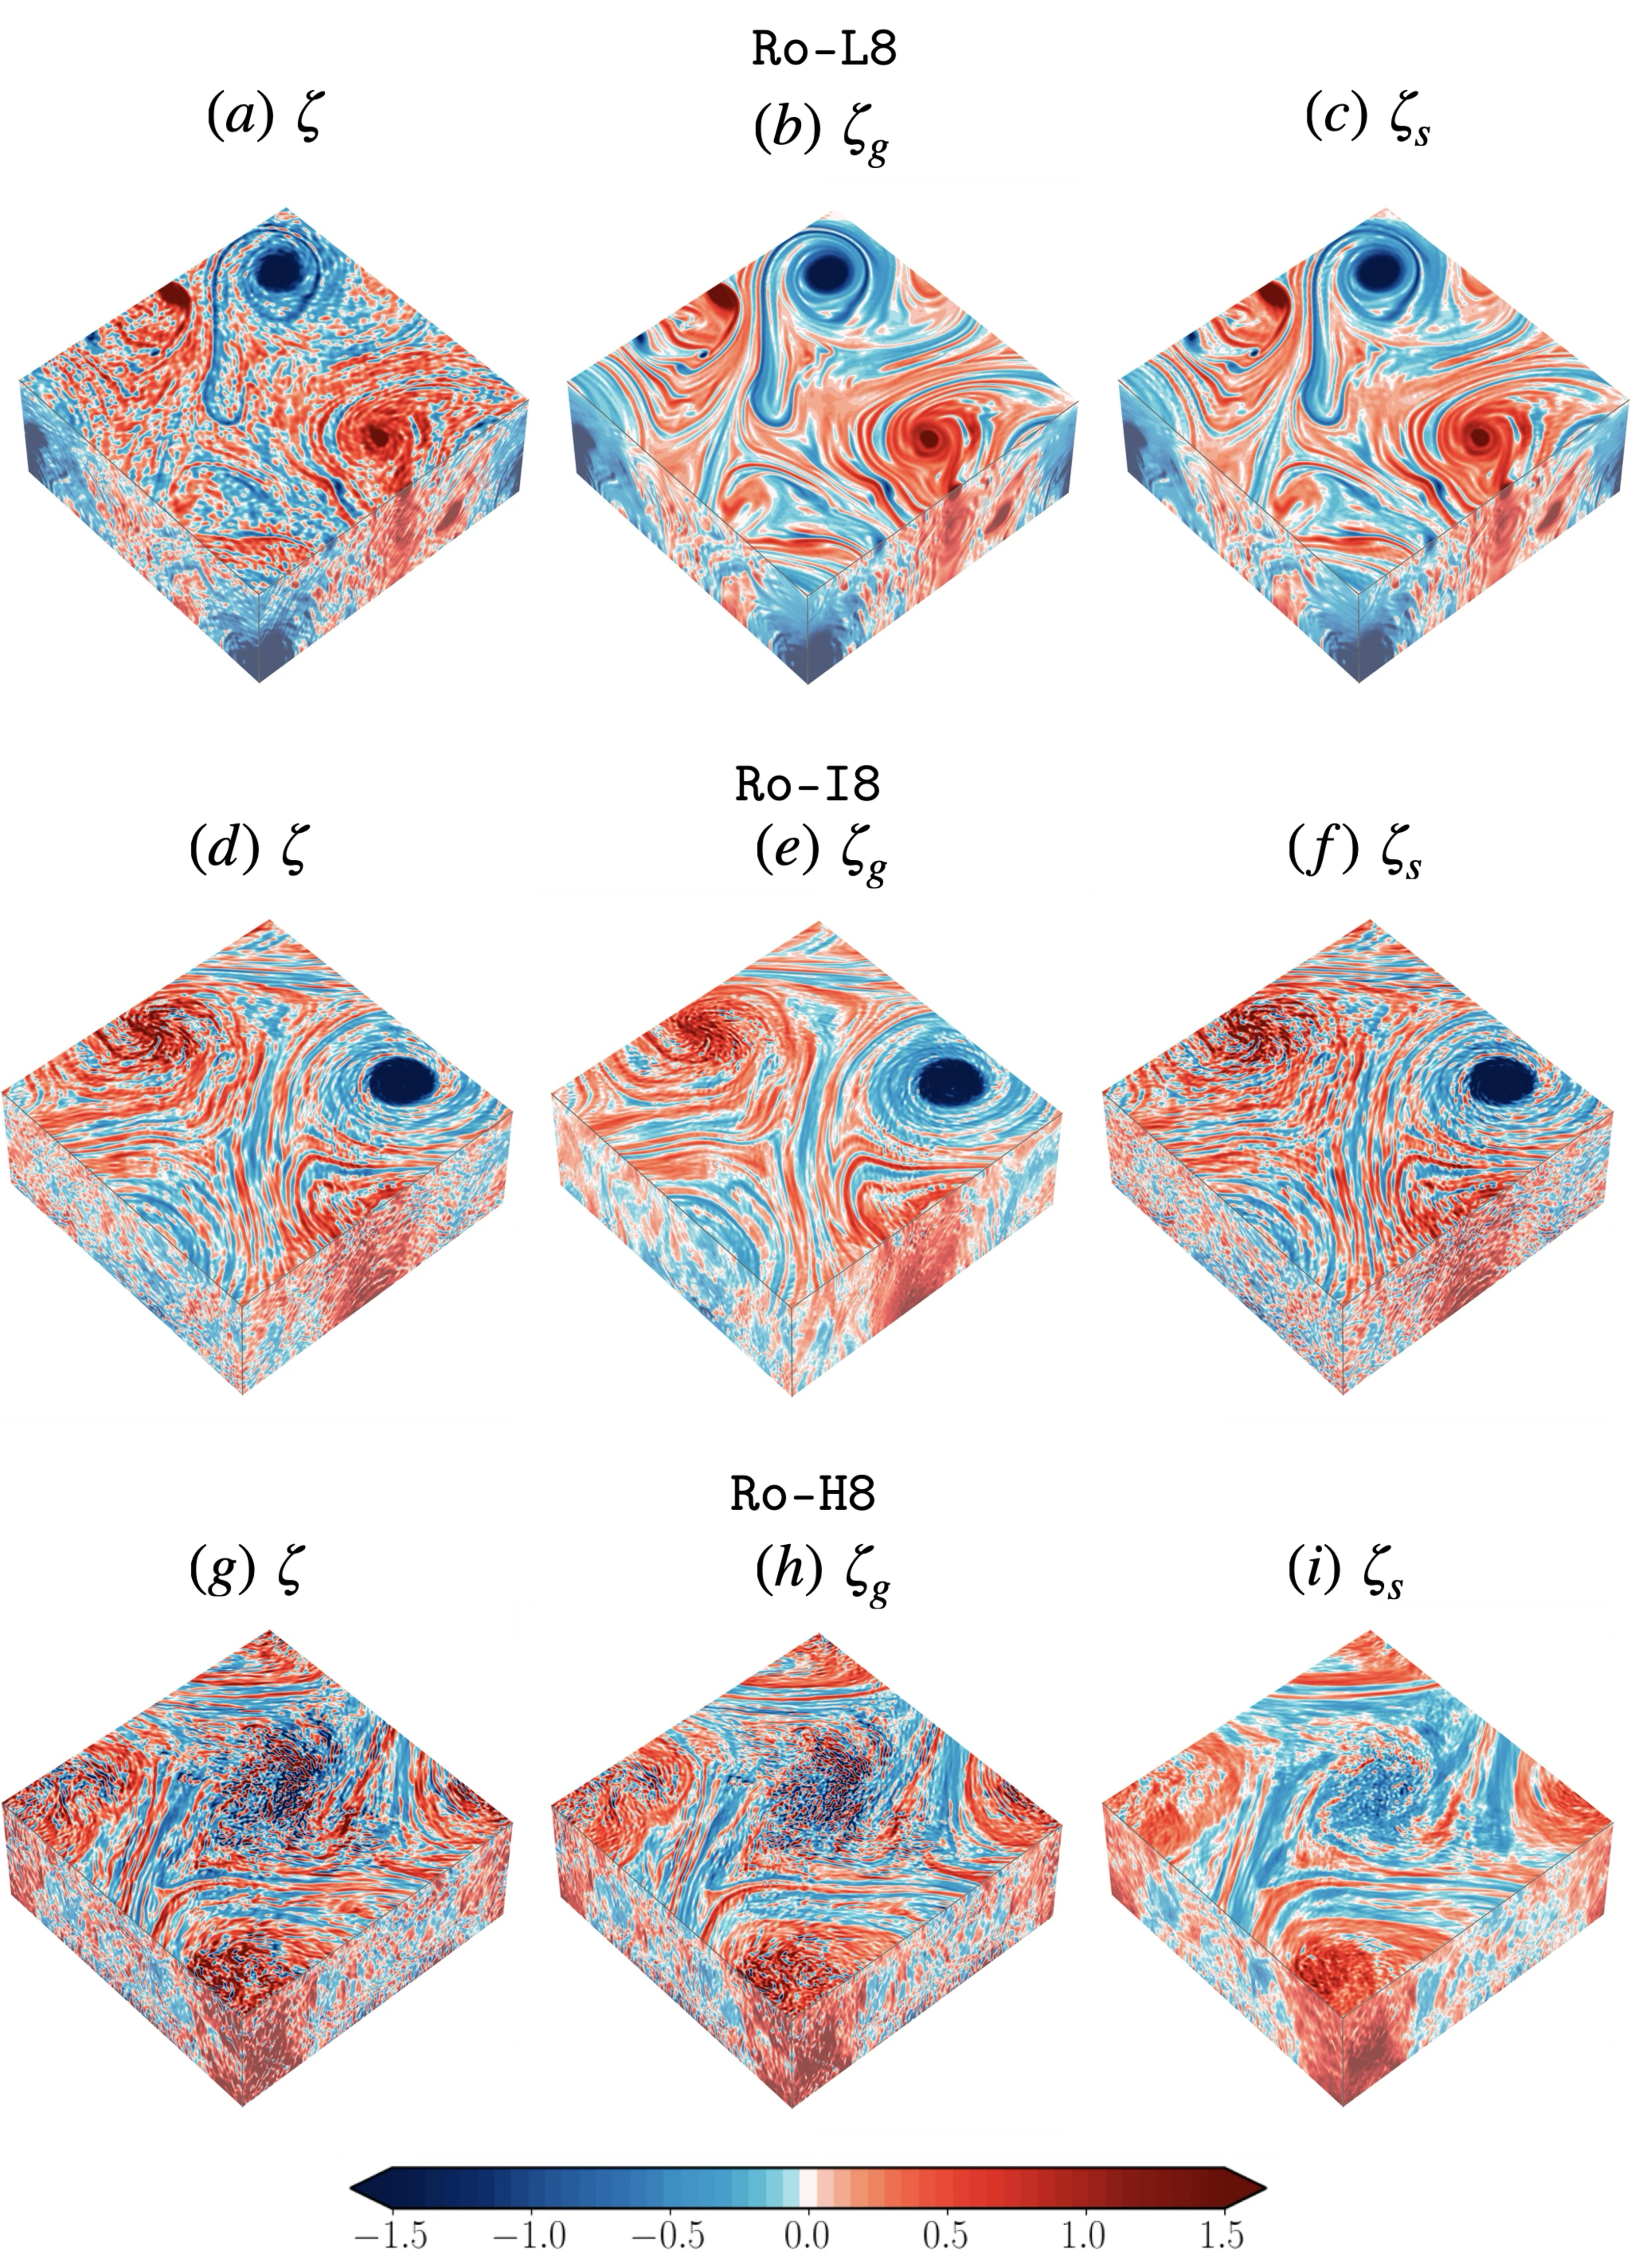
\includegraphics[width = 0.8\linewidth]{./figures/internal_tide_eddy/vorticity_lw_o_b_f_3d.pdf}
 \caption[Vertical vorticity of $E_g/E_a = 8$ flows with their geostrophic and slow parts]{ Vertical vorticity in the statistical stationary state for  $E_g/E_a = 8$ flows with low (top row), intermediate (middle row), and high (bottom row) Rossby numbers. The left column shows the full  vorticity, $\zeta$. The middle and the right columns show the vorticity of the geostrophic and the slow components, respectively. The top plane facing up is $z=-\pi/5$. 
 With increasing Rossby number, small-scale structures develop in the flow. At low and intermediate Rossby numbers, the geostrophic and slow components are similar to each other, with large-scale coherent vortices. At high Rossby number, the slow component captures coherent structures while the geostrophic component does not. }
 \label{edwv-psl}
 \end{figure}
 
 For \ire flow in Fig. \ref{edwv-psl}(d), we see straining regions with fine-scale structures develop around the coherent vortices. Notably, unlike the \lre flow, small-scale structures in the \ire flow persist in the geostrophic and the slow vorticity fields shown in Fig. \ref{edwv-psl}(e,f), respectively. Increasing Rossby number is therefore generating finer-scale structures in the slow-evolving eddies as well. Comparing panels (e) and (f), we see that the  geostrophic vorticity has fewer small-scale structures than the slow vorticity field. Therefore, the geostrophic field does a better job at capturing clear, large-scale structures than the slow field.  With further increase in Rossby number, we see that the \hre flow vorticity in Fig. \ref{edwv-psl}(g) has barely any coherent structures. This is true for $\zeta_g$ in Fig. \ref{edwv-psl}(h) as well. However, the slow component $\zeta_s$ in Fig. \ref{edwv-psl}(i) has prominent coherent structures with relatively less fine-scale features. Therefore, at higher Rossby numbers, when the full flow vorticity and the geostrophic vorticity are rich with fine-scale features, the slow flow vorticity still captures large-scale structures. 

 
 
 %This comparison highlights the significance of the slow-fast decomposition with regards to the physical flow structuyress: 
 
 
 %It also has fewer small-scale structures compared to the geostrophic component. We find that with increasing Rossby number, the net flow loses its coherent structure, but the slow component still captures the underlying coherent flow, while the geostrophic component does not. 
 
 
 %Between the geostrophic and the slow component, we see minor quantitative differences in the small-scale structures. Overall, they still look qualitatively similar. This is because the effective Rossby number of the flow is still small according to Table \ref{edwv-t1}. However, \ire flow tells us that the coherent eddies develop small-scale structures with increasing Rossby number. 
 
 

 Figure \ref{edwv-pse} similarly shows the physical structures for $E_g/E_a = 1$ flows. Rossby number increases from low to high as we move from the top row to the bottom row. Similar to its $E_g/E_a = 8$ counterpart, the low Rossby \lro flow in Fig. \ref{edwv-pse}(a) shows coherent vortices, although the small-scale structures in Fig. \ref{edwv-pse}(a) for \lro flow are much more than those seen in \lre flow in Fig. \ref{edwv-psl}(a). Many of these small-scale structures are absent in the geostrophic vorticity, $\zeta_g$, in Fig. \ref{edwv-pse}(b), signifying that the ageostrophic component generates the small-scale flow. Given that $E_g/E_a = 1$ flows have more ageostrophic motion than $E_g/E_a = 8$ flows, this also explains why $\zeta$ has more small-scale structures for the \lro flow. The slow component, $\zeta_s$, in Fig. \ref{edwv-pse}(c) also has clear large-scale coherent vortices, although we see slightly more fine-scale features than in the geostrophic vorticity seen in panel (b). 

% looks similar to the geostrophic component, once again emphasizing that at low Rossby numbers the slow geostrophic component is responsible for coherent eddies while fast ageostrophic flow component generates small-scale structures. % at low Rossby numbers coherent eddies in geostrophic and hydrostatic balance and evolve slowly. 

 

The \iro flow in Fig. \ref{edwv-pse}(d,e,f) is significantly different from its $E_g/E_a = 8$ counterpart. In Fig. \ref{edwv-pse}(d), $\zeta$ shows no coherent structures. The small-scale structures persist in the geostrophic component in Fig. \ref{edwv-pse}(e). However, the slow component in Fig. \ref{edwv-pse}(f) shows a large coherent anticyclonic eddy. The geostrophic and the slow components differ significantly for the \iro flow, which was not the case for \ire flow. This is because the \iro flow has more ageostrophic motion. With further increase in Rossby number, we see that the vorticity in Fig. \ref{edwv-pse}(g) for \hro flow has more small-scale structures, the geostrophic component in Fig. \ref{edwv-pse}(h) fails to get rid of them, whereas the slow component in Fig. \ref{edwv-pse}(i) shows prominent large-scale flow structures with relatively less small-scale features. 

\begin{figure}
\centering
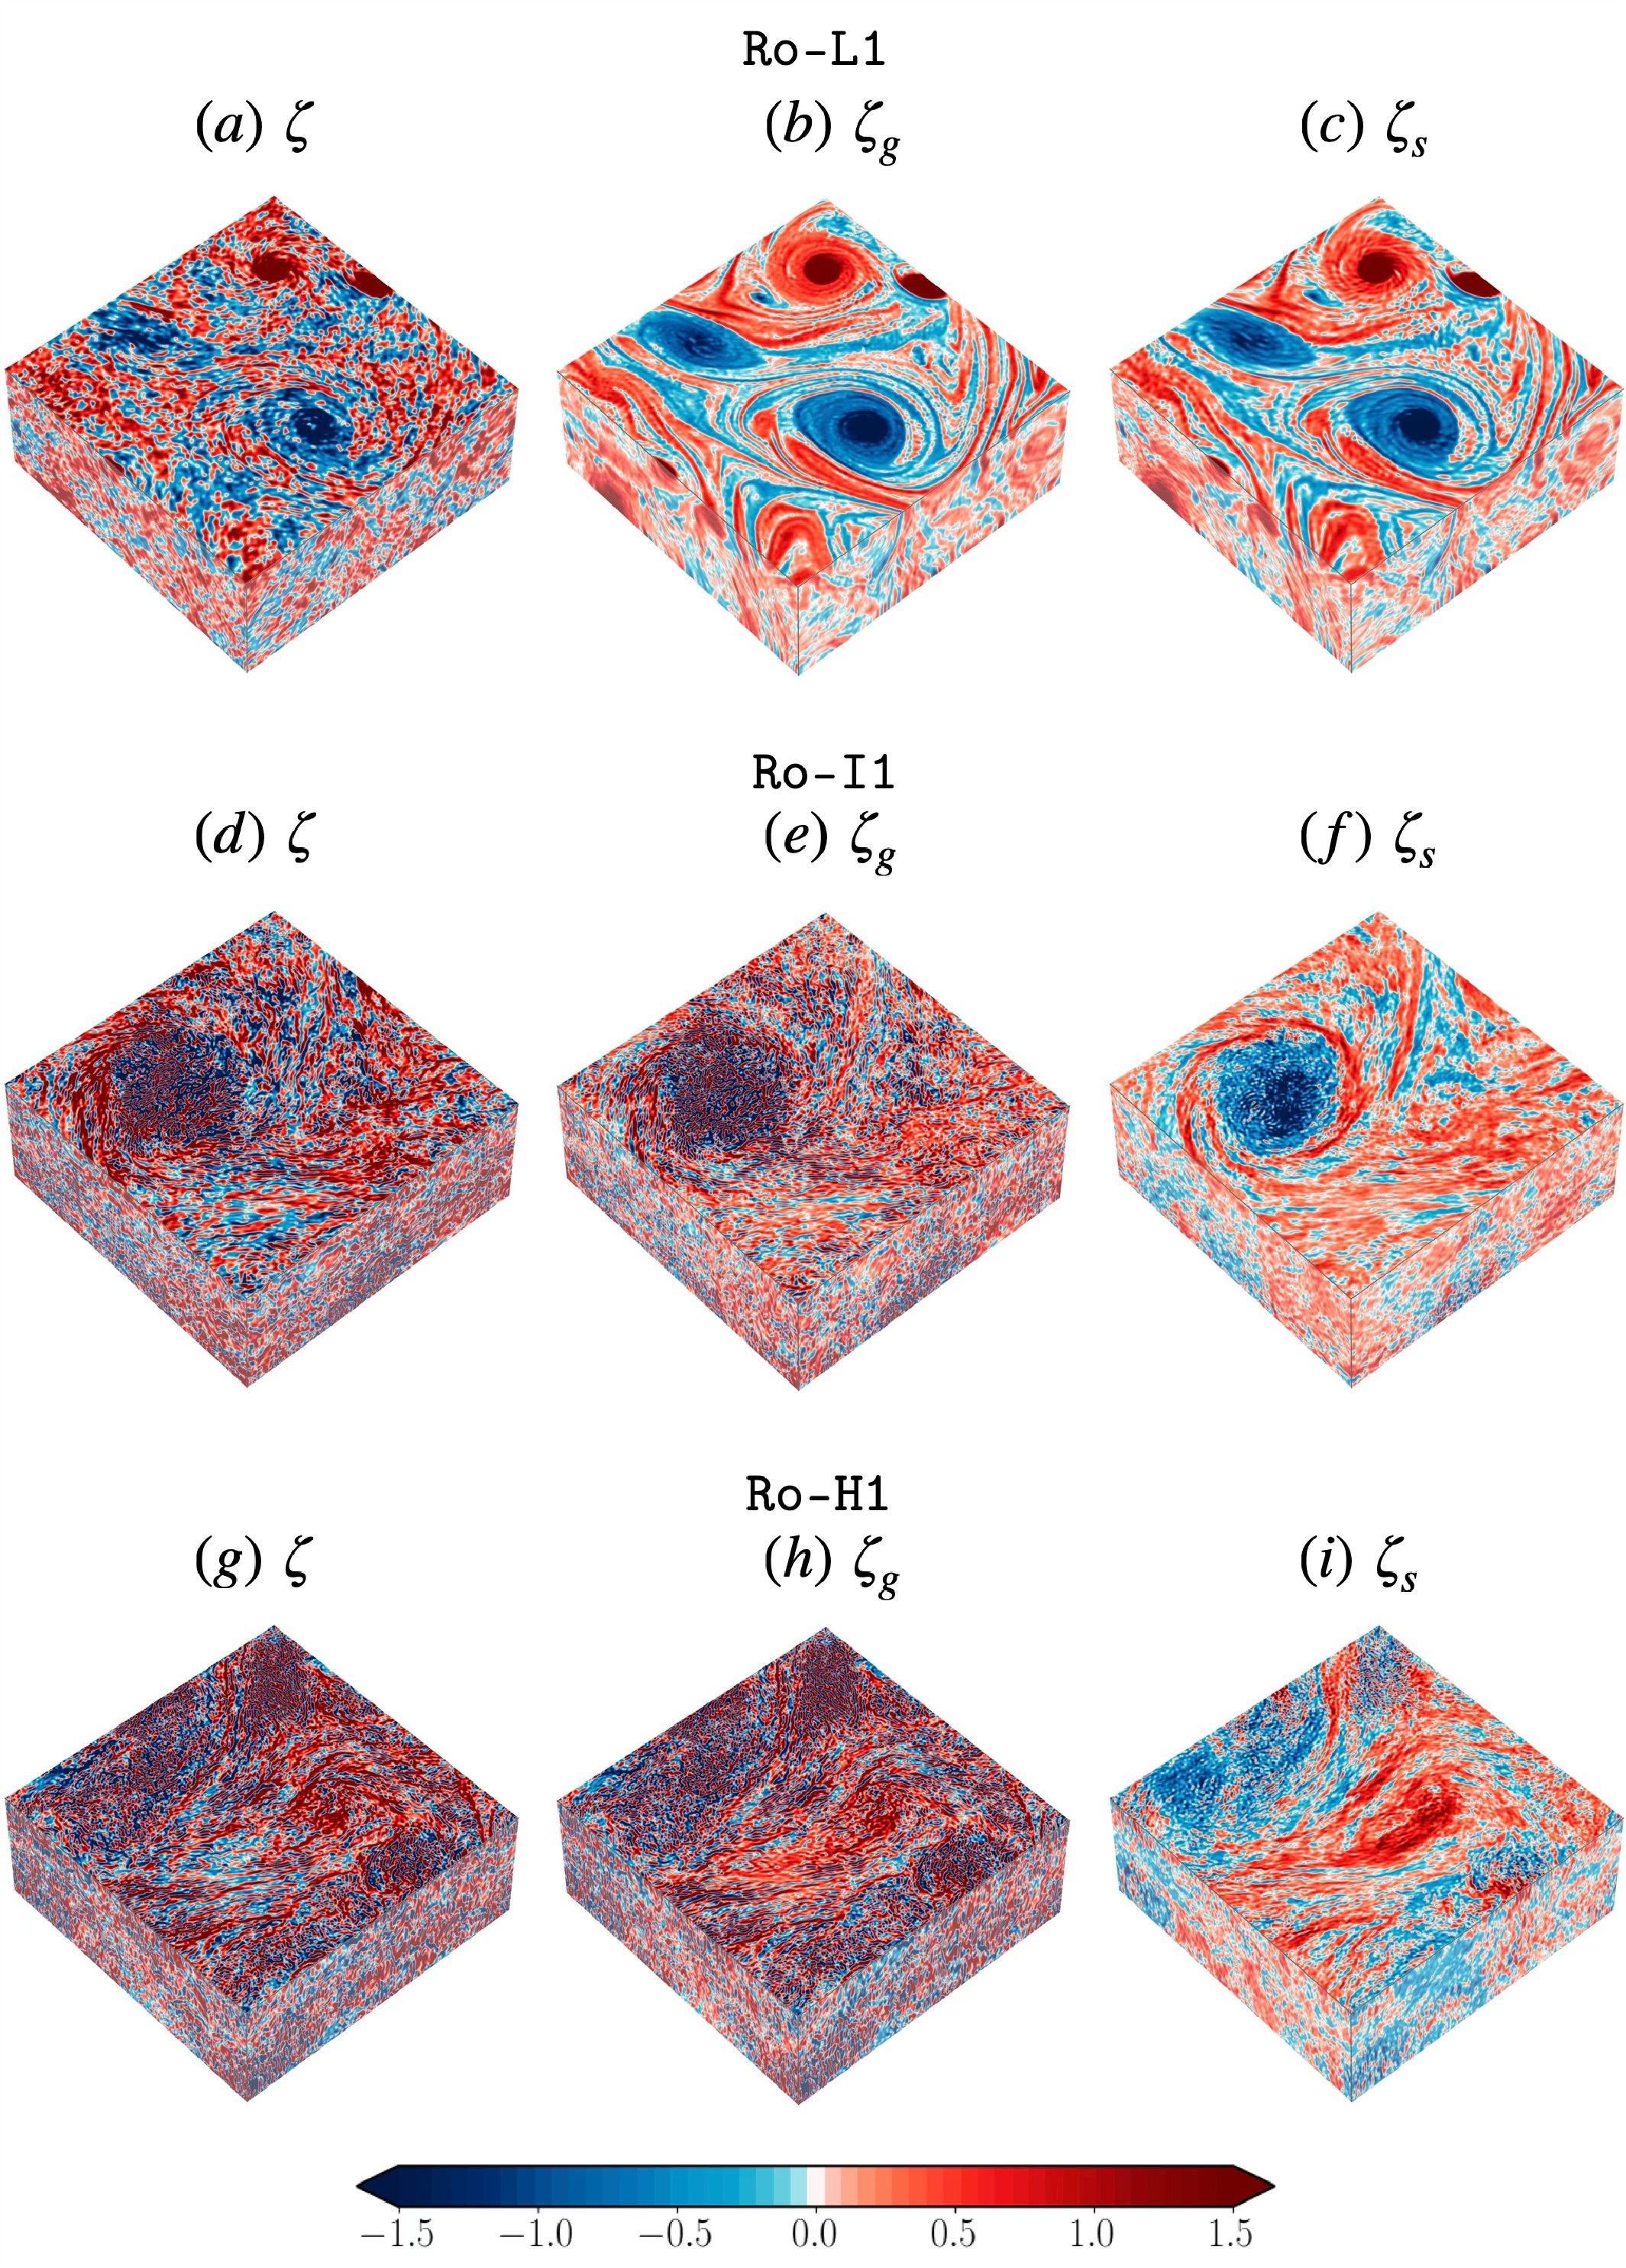
\includegraphics[width = 0.8\linewidth]{./figures/internal_tide_eddy/vorticity_ew_o_b_f_3d.pdf}
\caption[Vertical vorticity of $E_g/E_a = 1$ flows with their geostrophic and slow parts]{ Vertical vorticity in the statistical stationary state for  $E_g/E_a = 1$ flows with low (top row), intermediate (middle row), and high (bottom row) Rossby numbers. The left column shows the full  vorticity, $\zeta$. The middle and the right columns show the vorticity of the geostrophic and the slow components, respectively. The top plane facing up is $z=-\pi/5$. 
With increasing Rossby number, small-scale structures are pervasive in the flow, more than in $E_g/E_a = 8$ flows seen in the previous figure. The geostrophic and slow components match only for the low Rossby number \lro flow, both showing coherent structures. At intermediate and high Rossby numbers, only the slow component captures the coherent structures. }
\label{edwv-pse}
\end{figure}


The above examination of physical structures reveals that the geostrophic flow and slow flow are similar only at low Rossby numbers. Increasing Rossby number generates energetic small-scale features in the flow, also seen in the geostrophic flow, that lack coherent large-scale structures. The slow flow component, however, consistently captures large-scale structures even at high Rossby numbers, bringing out the usefulness of the slow-fast decomposition across Rossby numbers. Of course, the slow flow component also starts showing the presence of fine-scale features with increasing Rossby number, although they are much less than those seen in the full field and the geostrophic field. This limitation of the linear geostrophic-ageostrophic decomposition is expected, because it is derived from the linear equations. At intermediate and high Rossby numbers, flow components born out of strong nonlinear interactions are not well captured in this decomposition. We will next see how energetic interactions between the fields are in the different regimes.   %\rc{The next section studies how the energy interactions of the different flow components change fundamentally across Rossby number. We will see that the change in flow structures is a manifestation of a change in the flow interactions.}

%this being an indication of a strengthening forward energy cascade with Rossby number. 


%From the physical structures we see that the geostrophic-ageostrophic and the slow-fast decomposition are equivalent for low Rossby numbers flows \lre and \lro. As the Rossby number increases, only the slow component can capture the coherent structures in the flow. The geostrophic component fails to capture any coherent structure for the \hre, \iro, and \hro flows, whose $\roeff$ is more than $0.5$. This failure is due to nonlinear, ageostrophic motions that contribute to the linear potential vorticity at large Rossby numbers. They prevent the geostrophic-ageostrophic decomposition from accurately capturing the coherent high Rossby eddies, making the slow-fast decomposition more useful. Furthermore, with increasing Rossby number, slow components develop small-scale structures, indicating that for high Rossby number flows, coherent eddies start to break. 

% \begin{figure*}
% \centering
% \includegraphics[width=\linewidth]{./figures/internal_tide_eddy/vorticity_ro_0.1_lw_o_b_f.pdf}
% \caption{Vortiicty snapshot for $Ro = 0.1$ flow with low ageostrophic energy (left). The vorticity arising from the geostrophic component (middle) and the slow component (right) is shown to compare their contribution.}
% \label{edwv-fig:pstruc-0.1-lw}
% \end{figure*}

% \begin{figure*}
% \centering
% \includegraphics[width=1\linewidth]{./figures/internal_tide_eddy/vorticity_ro_0.5_lw_o_b_f.pdf}
% \caption{Vortiicty snapshot for $Ro = 0.5$ flow with low ageostrophic energy (left). The vorticity arising from the geostrophic component (middle) and the slow component (right) is shown to compare their contribution.}
% \label{edwv-fig:pstruc-0.5-lw}
% \end{figure*} 

% \begin{figure*}
% \centering
% \includegraphics[width=1\linewidth]{./figures/internal_tide_eddy/vorticity_ro_1.0_lw_o_b_f.pdf}
% \caption{Vortiicty snapshot for $Ro = 1.0$ flow with low ageostrophic energy (left). The vorticity arising from the geostrophic component (middle) and the slow component (right) is shown to compare their contribution.}
% \label{edwv-fig:pstruc-1.0-lw}
% \end{figure*}

% \begin{figure*}
% \centering
% \includegraphics[width=1\linewidth]{./figures/internal_tide_eddy/vorticity_ro_0.1_ew_o_b_f.pdf}
% \caption{Vortiicty snapshot for $Ro = 0.1$ flow with equal geostrophic-ageostrophic energy (left). The vorticity arising from the geostrophic component (middle) and the slow component (right) is shown to compare their contribution.}
% \label{edwv-fig:pstruc-0.1-ew}
% \end{figure*}
% \begin{figure*}
% \centering
% \includegraphics[width=1\linewidth]{./figures/internal_tide_eddy/vorticity_ro_0.5_ew_o_b_f.pdf}
% \caption{Vortiicty snapshot for $Ro = 0.5$ flow with equal geostrophic-ageostrophic energy (left). The vorticity arising from the geostrophic component (middle) and the slow component (right) is shown to compare their contribution.}
% \label{edwv-fig:pstruc-0.5-ew}
% \end{figure*}
% \begin{figure*}
% \centering
% \includegraphics[width=1\linewidth]{./figures/internal_tide_eddy/vorticity_ro_1.0_ew_o_b_f.pdf}
% \caption{Vortiicty snapshot for $Ro = 1.0$ flow with equal geostrophic-ageostrophic energy (left). The vorticity arising from the geostrophic component (middle) and the slow component (right) is shown to compare their contribution.}
% \label{edwv-fig:pstruc-1.0-ew}
% \end{figure*}

% Looking at the physical structures in Fig. \ref{edwv-psl}, \ref{edwv-pse}, we can draw the following conclusions. First, at low Rossby numbers, coherent large-scale cyclones and anticyclones form the mesoscale eddies. This is seen in the relative vorticity snapshots of both the geostrophic and the slow component of $Ro =0.1$ flows. For such flows, regardless of the geostrophic-ageostrophic energy ratio, the geostrophic and slow flows look almost identical, implying that at mesoscales, eddies evolve slowly and are in thermal wind balance. Even for the case of $E_g/E_a = 1$ in Fig. \ref{edwv-pse}, when there is significant ageostrophic flow and the net relative vorticity shows small-scale structures, both the slow-fast and the geostrophic-ageostrophic decompositions are competent enough to capture the mesoscale eddies.

% On the other hand, looking at the vorticity fields of higher Rossby numbers of $0.5$ and $1.0$ in Fig. (\ref{edwv-psl} and \ref{edwv-pse}), we find significantly more small-scale structures in the relative vorticity compared to their $Ro =0.1$ counterpart. These small-scale structures remain in the geostrophic component of the relative vorticity. This is in contrast with the idea that geostrophic eddies have large-scale structures. The slow component, in turn, has some large-scale coherent structures. Still, small-scale structures are present in the slow field as well. The presence of small-scale structures in both decompositions suggests that eddies break down at submesoscales. It also tells us that slow-fast decomposition is better at capturing submesoscale eddies ($Ro = 0.5, 1$) than the geostrophic-ageostrophic decomposition. This happens because at submesoscales, eddies need not be in thermal wind balance, and the eddy-wave interaction can generate significant nonlinear flows that can momentarily be in thermal wind balance.


 

\section{Energy transfers and dissipation}\label{edwv-cmp}

We will now explore the distribution of energy across scales using the horizontal energy spectrum, $\hat{E}(k_h, t)$, defined as 
\begin{align}
    % \label{}
    \begin{split}
        \hat{E}(k_h, t) = \sum\limits_{\theta_{k_h},k_z} \frac12 \left( |\hat{u}|^2 + |\hat{v}|^2 + \frac{|\hat{w}|^2}{\alpha^2}+ |\hat{b}|^2\right) \ ,
    \end{split}
\end{align}
where the hat denotes a Fourier-transformed quantity. $\theta_{k_h} = \tan^{-1}(k_y/k_x)$ is the azimuthal angle of any horizontal wavenumber $\vec{k}_h = (k_x,k_y)$, with wavenumber $|\vec{k}_h|$ within $k_h \pm 0.5$. The above summation over azimuthal angles and vertical wavenumbers is performed to obtain the horizontal energy spectrum. In addition to the full flow fields, we can construct horizontal energy spectra for different flow components. The geostrophic-ageostrophic components of the horizontal energy spectra are defined as 
\begin{subequations}
    % \label{}
    \begin{align}
        \begin{split}
            \hat{E}_{g}(k_h, t) = \sum\limits_{\theta_{k_h},k_z} \frac12\left( |\hat{u}_g|^2 + |\hat{v}_g|^2 + \frac{|\hat{w}_g|^2}{\alpha^2}+ |\hat{b}_g|^2\right)
        \end{split} \\
        \begin{split}
            \hat{E}_{a}(k_h, t) = \sum\limits_{\theta_{k_h},k_z} \frac12 \left( |\hat{u}_a|^2 + |\hat{v}_a|^2 + \frac{|\hat{w}_a|^2}{\alpha^2}+ |\hat{b}_a|^2\right) \ , 
        \end{split}
    \end{align}
\end{subequations}
 With the above, we have $\hat{E}(k_h, t) = \hat{E}_{g}(k_h, t) + \hat{E}_{a}(k_h, t)$ at every instant of time (see details given in appendix \ref{edwv-budet}). Similarly, we can define the slow and the fast components of the horizontal energy spectra as 
\begin{subequations}
    % \label{}
    \begin{align}
        \begin{split}
            \hat{E}_{s}(k_h, t) = \sum\limits_{\theta_{k_h},k_z} \frac12 \left( |\hat{u}_s|^2 + |\hat{v}_s|^2 + \frac{|\hat{w}_s|^2}{\alpha^2}+ |\hat{b}_s|^2\right)
        \end{split} \\
        \begin{split}
            \hat{E}_{f}(k_h, t) = \sum\limits_{\theta_{k_h},k_z} \frac12 \left( |\hat{u}_f|^2 + |\hat{v}_f|^2 + \frac{|\hat{w}_f|^2}{\alpha^2}+ |\hat{b}_f|^2\right) \ . 
        \end{split}
    \end{align}
\end{subequations}
However, as mentioned before, unlike the geostrophic-ageostrophic decomposition, $\hat{E}(k_h, t) \neq \hat{E}_{s}(k_h, t) + \hat{E}_{f}(k_h, t)$. Instead, following  the discussions in \S \ref{edwv-sfdcmp}, $\bar{\hat{E} }(k_h) = \bar{\hat{E}_{s} }(k_h) + \bar{\hat{E}_{f}}(k_h)$, where over-bar denotes the time-averaging operation. The left columns of Figs. \ref{edwv-ekl} and \ref{edwv-eke} show time-averaged horizontal spectra, along with their slow-fast and geostrophic-ageostrophic components for the six flow regimes.

\begin{figure}
	\centering
	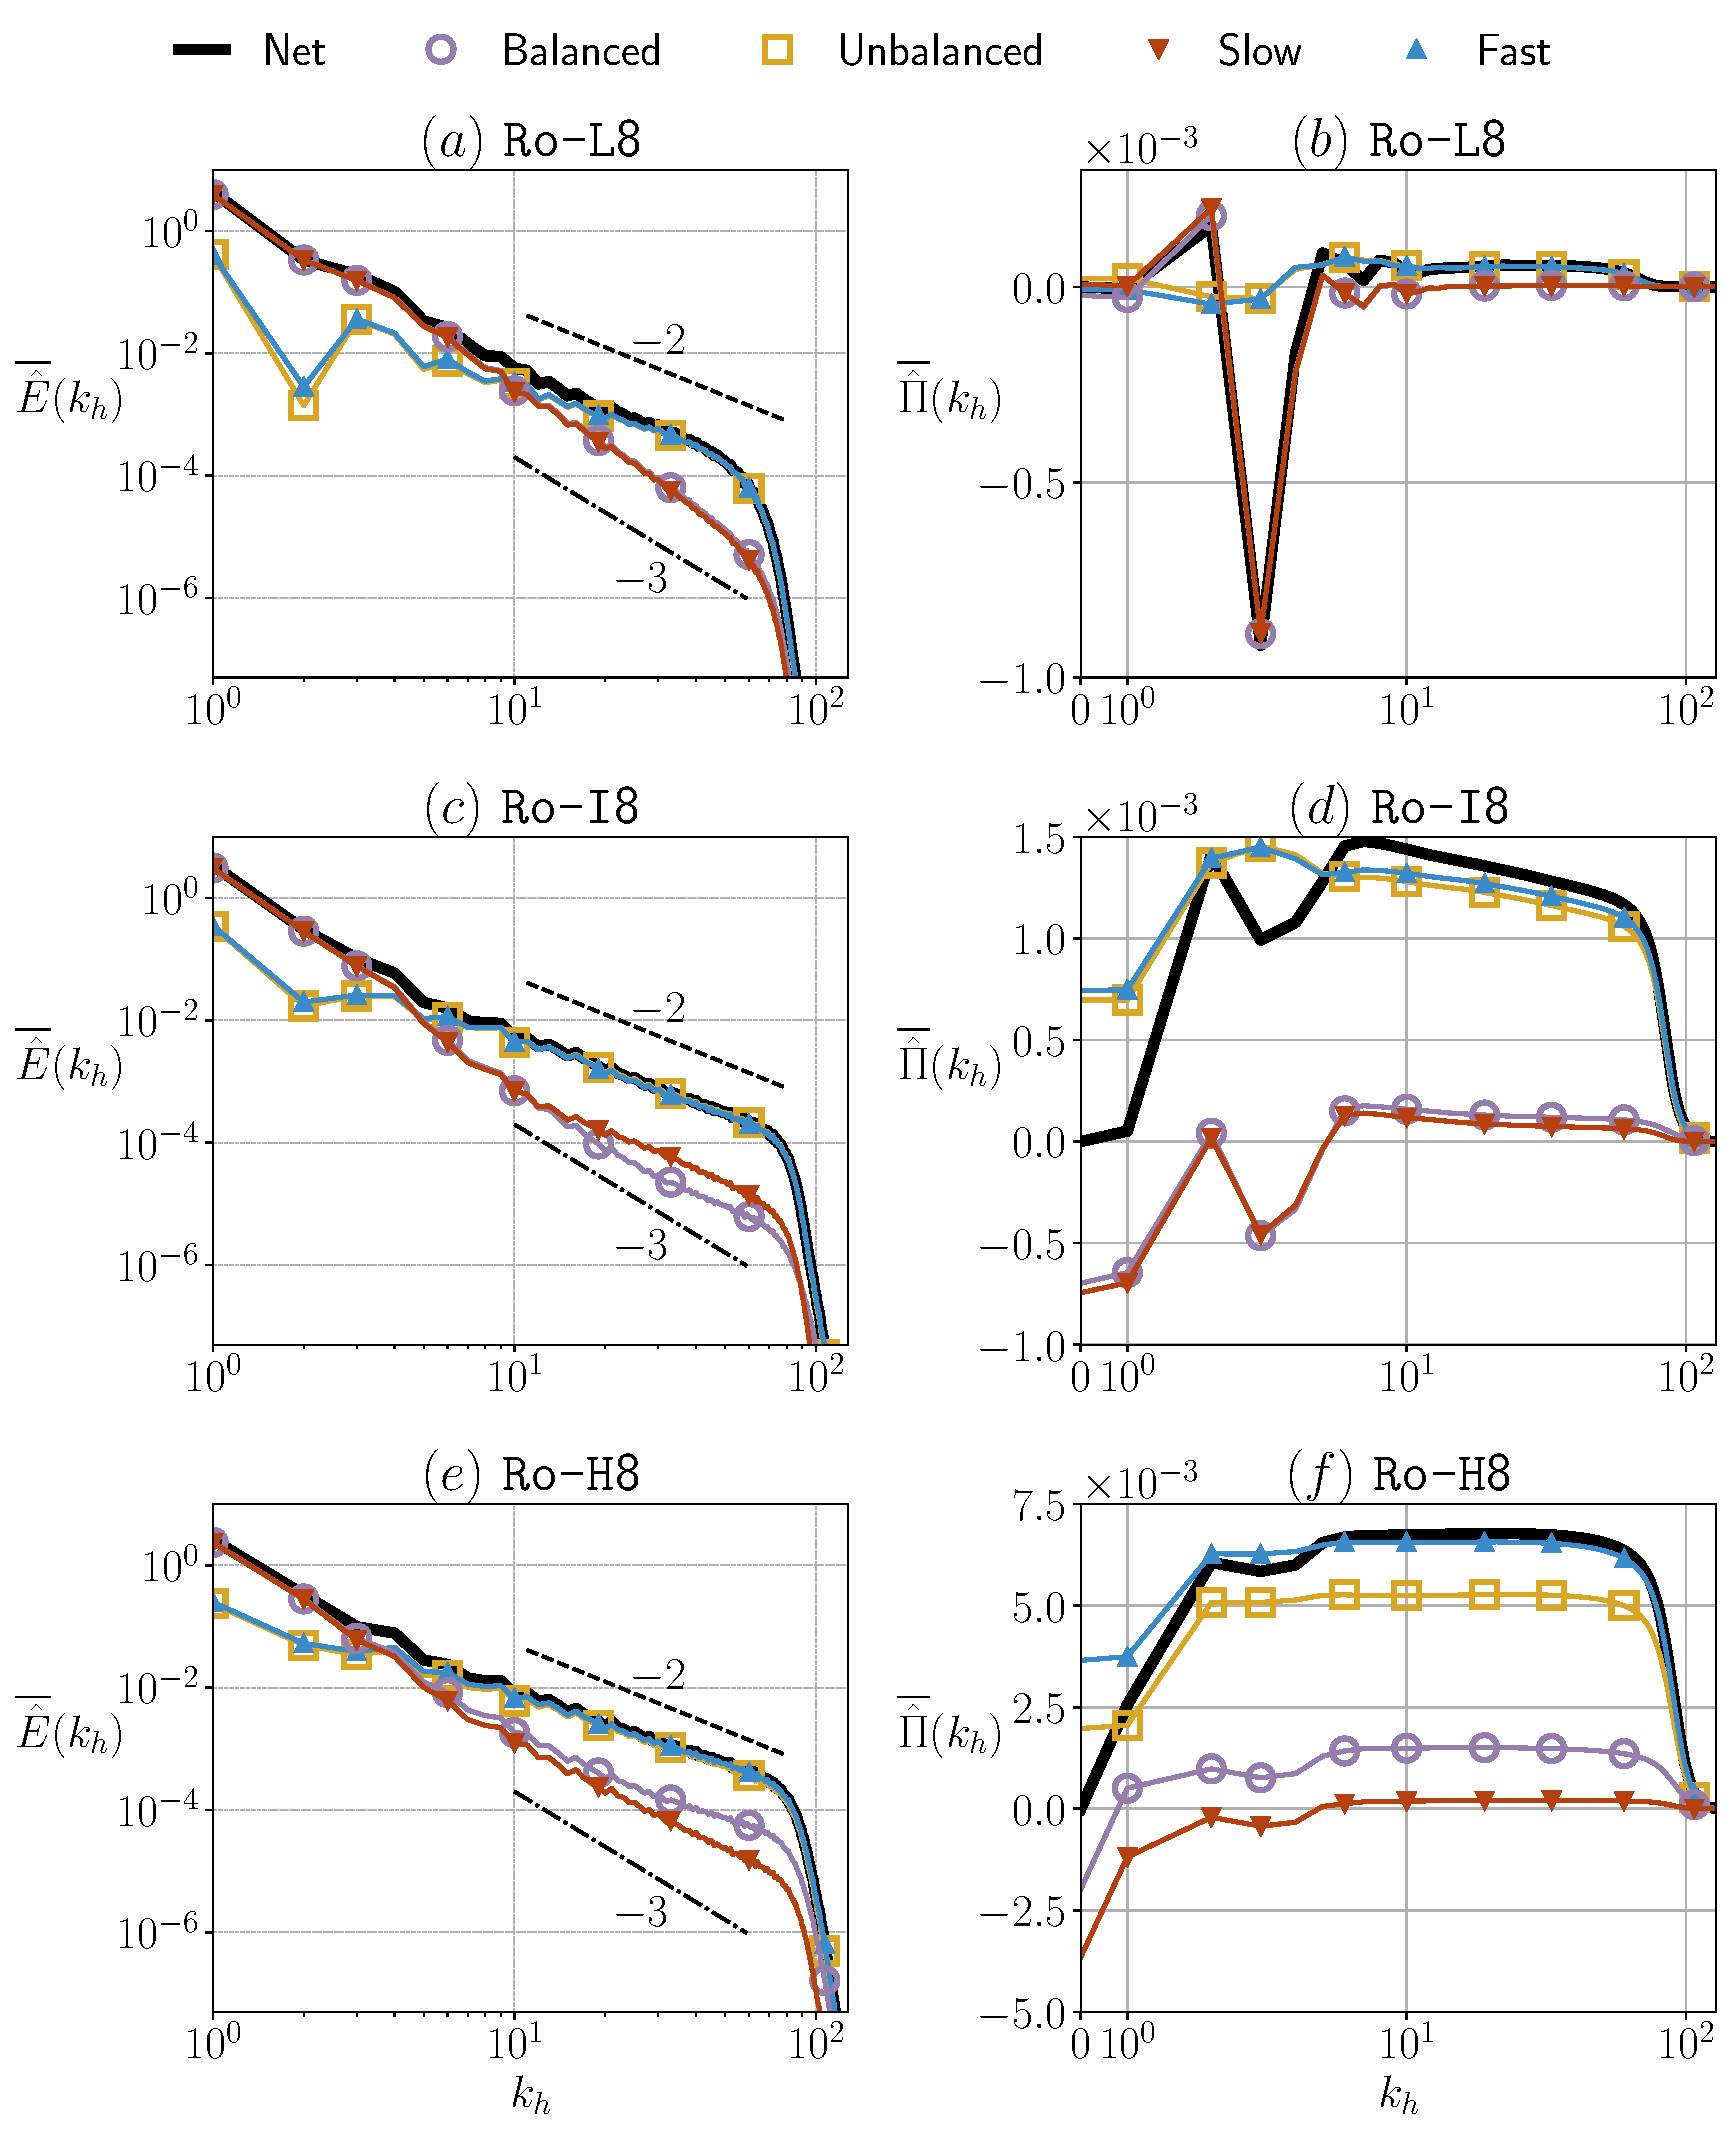
\includegraphics[width=1\linewidth]{./figures/internal_tide_eddy/ekh_pikh_wb_fs_lw.pdf}
	\caption[Horizontal energy spectra and spectral energy flux for $E_g/E_a = 8$ flows]{ Time-averaged horizontal energy spectra (left) and horizontal spectral flux (right) for $E_g/E_a = 8$ flows.  Rossby number changes from low (\lre, top row), to intermediate (\ire, middle row), to high (\hre, bottom row). The different colors show different components of the energy spectra and spectral flux. A positive flux represents a downscale cascade while a negative flux represents an upscale cascade.} % At high Rossby, the geostrophic spectra deviates from the slow component at large wavenumbers, and becomes similar to the ageostrophic and the fast spectra. With increasing Rossby number, the positive fast flux dominates the negative slow flux, generating more small-scale structure in the flow. At high Rossby, the geostrophic flux is positive and generates the small-scale structures. The magnitude of the flux increases with Rossby number. }
\label{edwv-ekl}
\end{figure}

Figure \ref{edwv-ekl}(a) corresponds to the \lre flow with $E_g/E_a = 8$. The fast and the ageostrophic components in blue and yellow, respectively, almost overlap with each other. The same is true for the slow and the geostrophic components in red and purple, respectively. This is a direct result of the fact that at low Rossby numbers, eddies evolve slowly and are in geostrophic and hydrostatic balance. Therefore, both the geostrophic and the slow components essentially capture the same part of the flow. The ageostrophic and the fast components match as they are the remaining parts of the flow after subtracting the geostrophic and the slow components, respectively. Furthermore, from the spectra, we see that the ageostrophic and the fast flow dominate for wavenumbers above $k_h = 10$. At these higher wavenumbers, the ageostrophic and the fast spectra scale close to $k_{h}^{-2}$, while their geostrophic and slow counterparts scale as $k_h^{-3}$.

At intermediate Rossby number, for \ire flow in Fig. \ref{edwv-ekl}(c), we see a behavior similar to the \lre flow for the fast and ageostrophic fields. However, the geostrophic spectrum is slightly steeper than the slow spectrum, this being a reflection of more small-scale structures seen in the slow field than the geostrophic field in the second row of figure \ref{edwv-psl}. 
For \hre flow with even higher Rossby number, the spectra are shown in Fig. \ref{edwv-ekl}(e). Notice that the slow spectrum is steeper than the geostrophic spectrum at higher wavenumbers. Looking back at the third row of figure \ref{edwv-psl}, we see that the slow component has larger scale structures than the geostrophic component at this high Rossby number, leading to the slow spectrum being steeper than the geostrophic spectrum.  The spectra also show that the fast and ageostrophic spectra overlap across scales. 

For the flows with $E_g/E_a = 1$, we see in Fig. \ref{edwv-eke}(a) that for the \lro flow, the two decompositions lead to similar outcomes. The geostrophic and the slow components, in purple and red, respectively, are similar at large scales.  At scales below  $k_h = 30$, we see that the slow spectrum is slightly shallower. As Rossby number increases for \iro flow, in Fig. \ref{edwv-eke}(c), we see significant differences in the two decompositions. For scales below  $k_h = 10$, the geostrophic component in purple deviates from the $k_h^{-3}$ slope and becomes shallower. It scales close to $k_h^{-2}$, similar to the ageostrophic and the fast components in yellow and blue, respectively. The slow component in red is steeper than the geostrophic component and stays close to the $k_h^{-3}$ line. This is due to the small-scale structures in the geostrophic component of the flow at this Rossby number in Fig. \ref{edwv-pse}(e), whereas the slow component, in Fig. \ref{edwv-pse}(f), has large-scale coherent structures. The difference in the slow and geostrophic components is further seen in Fig. \ref{edwv-eke}(e), where in the \hro flow, the geostrophic component in purple shallows further up, while the slow component in red remains close to the $k_h^{-3}$ scaling. Although the slow and geostrophic spectra deviate with increasing Rossby number, the fast and ageostrophic components' spectra agree reasonably well, as seen in the three regimes shown in the left column of Fig. \ref{edwv-eke}. 

\begin{figure}
\centering
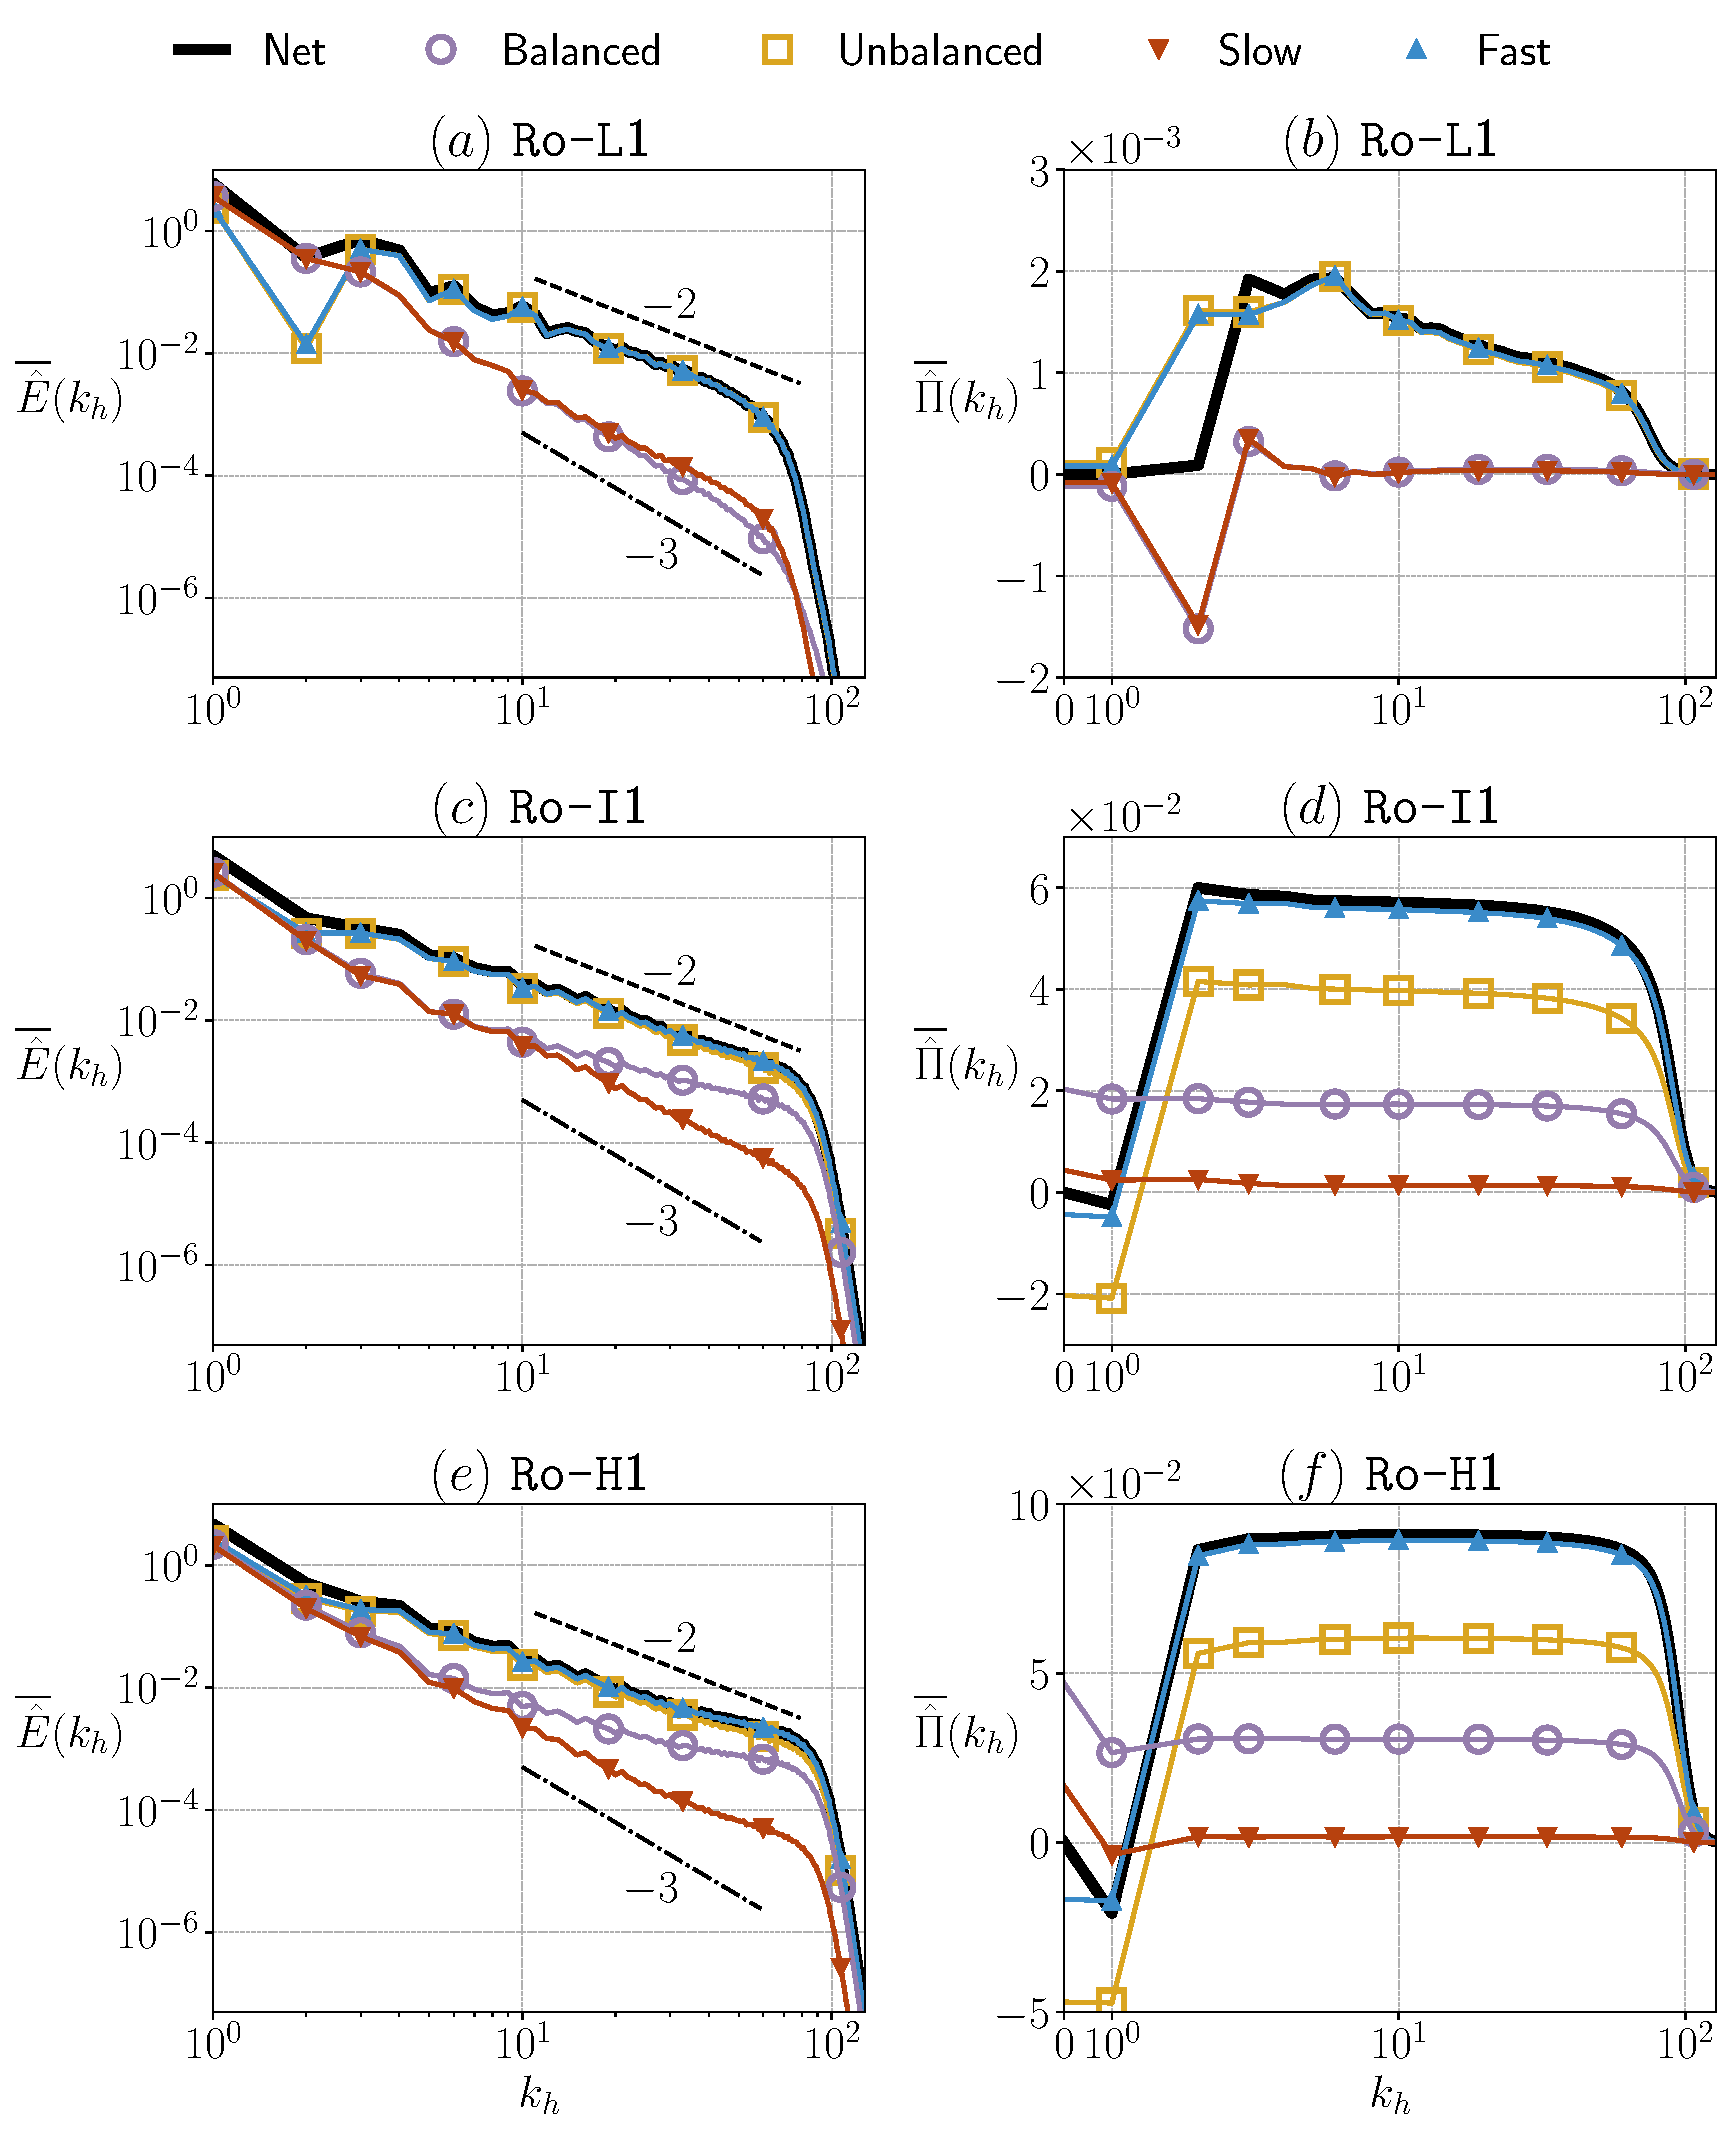
\includegraphics[width=1\linewidth]{./figures/internal_tide_eddy/ekh_pikh_wb_fs_ew.pdf}
\caption[Horizontal energy spectra and spectral energy flux for $E_g/E_a = 1$ flows]{ Time-averaged horizontal energy spectra (left) and horizontal spectral flux (right) of $E_g/E_a = 1$ flows.  Rossby number changes from low (\lro, top row), to intermediate (\iro, middle row), to high (\hro, bottom row). The different colors show different components of the energy spectra and spectral flux. A positive flux represents a downscale cascade while a negative flux represents an upscale cascade.} %For intermediate and high Rossby number flows, the geostrophic spectra deviates from the slow component at large wavenumbers, and becomes similar to the ageostrophic and the fast spectra. The slow flux at intermediate and high Rossby is negligible compared to the fast flux. The geostrophic flux becomes significant and positive for \iro and \hro, generating significant small-scale flows. The magnitude of the flux increases with Rossby number.}
\label{edwv-eke}
\end{figure}

We will next look at the energy transfer rate across scales for the flow components. For this, we take the Fourier transform of \eqref{edwv-bsnq}, multiply it with complex conjugates of velocity and buoyancy amplitudes, and take its real part to write down the following energy budget equation:
\begin{align}
\label{edwv-spebg}
\begin{split}
\frac{d }{dt}\hat{E}(k_h, t) = \hat{T}(k_h, t) + \hat{F}(k_h, t) - \hat{D}(k_h, t) ,
\end{split}
\end{align}
where $\hat{F}, \hat{D}$, and $\hat{T}$ are the power input, dissipation, and the energy gained or lost through nonlinear transfer in wavenumber $k_h$ given by 
\begin{subequations}
\begin{align}
% \label{}
\begin{split} 
    \hat{F}(k_h, t) = \sum\limits_{\theta_{k_h}k_z} \op{Re}\left(\hat{\vec{v}}_k^*.\hat{\vec{F}}_{u} + \frac{\hat{w}_k^*\hat{F}_w}{\alpha^2} + \hat{b}_k^*\hat{F}_b\right) 
\end{split}
\end{align}
\begin{align}
\begin{split}
    \hat{D}(k_h, t) = \nu\sum\limits_{\theta_{k_h}k_z} (k_h^{16} + k_z^{16})\left( |\hat{u}|^2 + |\hat{v}|^2 + \frac{|\hat{w}|^2}{\alpha^2}+ |\hat{b}|^2\right)
\end{split}
\end{align}
\begin{align}
\begin{split}
    \hat{T}(k_h, t) = \sum\limits_{\theta_{k_h}k_z} \op{Re}\left( \hat{\vec{v}}_k^* . \hat{\vec{R}}_{v} + \frac{\hat{w}_k^*\hat{R}_w}{\alpha^2} + \hat{b}_k^*\hat{R}_b \right) \ .
\end{split}
\end{align}
\end{subequations}
where $\hat{\vec{R}}_{\vec{v}}, \hat{R}_w$, and $\hat{R}_b$ are the Fourier transforms of the nonlinear terms in the evolution equations of $\vec{v}, w$, and $b$, respectively, in \eqref{edwv-bsnq}. The nonlinear transfer term $\hat{T}$ conserves the total energy. Thus, if some wavenumbers lose energy due to nonlinear transfers, other wavenumbers must gain an equal amount of energy. If $k_m$ is the maximum wavenumber present in the system, $\sum_{0}^{k_m} \hat{T}(k_h, t) = 0$. The horizontal spectral flux, $\hat{\Pi}(k_h, t)$, represents the rate at which wavenumbers smaller than $k_h$ lose energy to wavenumbers larger than $k_h$. It is defined by
\begin{align}
% \label{}
\begin{split}
\label{edwv-fxe}
\hat{\Pi}(k_h, t) = \sum\limits_{s=k_h}^{k_m} \hat{T}(s, t) = - \sum\limits_{s=0}^{k_h} \hat{T}(s, t) \ .
\end{split}
\end{align}

According to the above definition, a positive spectral flux at a particular length scale signifies forward energy transfer from that scale to smaller ones, while a negative flux signifies the opposite. From the Boussinesq equations, \eqref{edwv-bsnq}, we calculated $\hat{T}(k_h, t)$ for the geostrophic and ageostrophic components separately. This then allows us to calculate the geostrophic and the ageostrophic flux, $\hat{\Pi}_g(k_h, t)$ and $\hat{\Pi}_a(k_h, t)$, respectively. Due to the nature of the geostrophic-ageostrophic decomposition, $\hat{\Pi}_g(k_h, t) + \hat{\Pi}_a(k_h, t) = \hat{\Pi}(k_h, t)$. Similarly, one can also write down the rate of change of the slow and the fast energy components, which can then be used to calculate the slow and the fast components of the horizontal spectral flux $\hat{\Pi}_s(k_h, t)$ and $\hat{\Pi}_f(k_h, t)$, respectively. Again, similar to the case of energy spectra,  $\hat{\Pi}_s(k_h, t) + \hat{\Pi}_f(k_h, t) \neq \hat{\Pi}(k_h, t)$ instantaneously. Instead, $\bar{\hat{\Pi}_s}(k_h) + \bar{\hat{\Pi}_f}(k_h) = \bar{\hat{\Pi}}(k_h)$. The time-averaged net spectral flux and its different components for the six flow regimes are shown in the right column of Figs. \ref{edwv-ekl} and \ref{edwv-eke}.

Figure \ref{edwv-ekl}(b) shows the spectral flux and its components for \lre flow. It has a large negative flux at small wavenumbers, signifying an inverse energy cascade. The entirety of the negative flux is due to the geostrophic and the slow components in purple and red, respectively. These two components overlap, as seen before in the case of the energy spectra and the physical structure. The ageostrophic and the fast components are also similar and generate a small constant positive flux at scales below  $k_h \approx 10$. %The constant flux signifies the presence of an inertial range across these wavenumbers. 
These results further confirm that at low Rossby numbers, the slowly evolving geostrophic component undergoes an inverse cascade, leading to large-scale coherent eddies, whereas the rapidly evolving ageostrophic component undergoes a forward cascade and generates small-scale flow structures.


Increasing the Rossby number, for \ire flow in Fig. \ref{edwv-ekl}(d), positive downscale flux coming from the ageostrophic and the fast components now dominate the net flux. At low wavenumbers below $k_h =10$, the geostrophic and the slow components have negative flux. However, it is neutralized by the large positive flux of the ageostrophic and the fast components, respectively. These effects are exemplified for the \hre flow in Fig. \ref{edwv-ekl}(f), where the large positive flux of the ageostrophic and the fast components dominate the net flux at all wavenumbers. Figure \ref{edwv-ekl}(f) also shows the difference between the geostrophic and the slow components. In addition to the negative flux signifying the inverse cascade at small wavenumbers, the geostrophic component also has positive flux at large wavenumbers. This positive flux explains why the geostrophic component in Fig. \ref{edwv-psl}(h) has small-scale structures. The slow component, on the other hand, has negative flux at small wavenumbers and a negligible positive flux at large wavenumbers. This generates and sustains the large-scale structures seen in  Fig. \ref{edwv-psl}(i). It is also noteworthy that increasing Rossby number increases the net flux magnitude across Fig. \ref{edwv-ekl}(b,d,f), indicating the strengthening of the forward energy cascade. 

The forward cascade further increases in strength as we go from $E_g/E_a = 8$ flows to $E_g/E_a = 1$ flows. In Fig. \ref{edwv-eke}(b), for \lro flow, the geostrophic and the slow components overlap. They have negative flux at low wavenumbers, below $k_h = 10$, and minimal flux at high wavenumbers. The ageostrophic and fast components of the flux also overlap and show positive flux across all wavenumbers. The typical magnitude of the forward flux in Fig. \ref{edwv-eke}(b) is larger than the flux of \lre flow in Fig. \ref{edwv-ekl}(b), because there is more ageostrophic energy in the \lro flow. Going to the intermediate Rossby number in \iro flow, in Fig. \ref{edwv-eke}(d), we see that the magnitudes of the net flux further increase. The positive flux of the ageostrophic and the fast components also increases in magnitude. The geostrophic component in purple now shows a positive flux across all wavenumbers, and its magnitude is comparable to the ageostrophic flux. The slow component in red also shows positive flux, but the value is negligible compared to the fast flux.  The forward cascade of the geostrophic component generates the small-scale structures in Fig. \ref{edwv-pse}(e). The flux for high Rossby number flow, \hro,  in Fig. \ref{edwv-eke}(f) follows a similar trend, with the magnitude of the fluxes further increasing. The slow component has negligible positive flux, while the geostrophic component has a forward flux at all wavenumbers. This further explains why the slow-fast decomposition was successful in capturing slow-evolving coherent flows at large Rossby numbers in the physical structure visualizations seen earlier. 

We now turn to investigate the time-averaged dissipation, $\bar{D}$,  of different flow components in  Figs. \ref{edwv-dt}(a) and (b). Notice that in each panel, the net dissipation increases by two orders of magnitude as we go from \lr to \hr flows. Comparing panels (a) and (b), we see that increasing ageostrophic flow energy increases the net dissipation, as the $E_g/E_a = 1$ flows show one order of magnitude more dissipation than the $E_g/E_a = 8$ flows at each Rossby number. This is expected as the ageostrophic motion dominates the forward flux in Figs. \ref{edwv-ekl} and \ref{edwv-eke}. Consequently, they are also the major contributors to the net dissipation in Figs. \ref{edwv-dt}(a) and (b). The same is true for the fast component. They dominate the forward flux, and their dissipation eclipses the slower component's dissipation by orders of magnitude at all Rossby numbers. \cite{wang2025a} also found this in observations and realistic simulations, where eddies scatter and distort low mode internal tides to produce small-scale fast motions which enhance flow dissipation.  Also note that the geostrophic component in Fig. \ref{edwv-dt} shows different behavior than the slower component at intermediate and high Rossby numbers. Although its dissipation is lower than the ageostrophic component, it is considerably higher than the slow component for \hre, \iro, and \hro flows. This is due to the considerable forward flux they generate at these Rossby numbers, which leads to enhanced dissipation.  


\begin{figure}
	\centering
	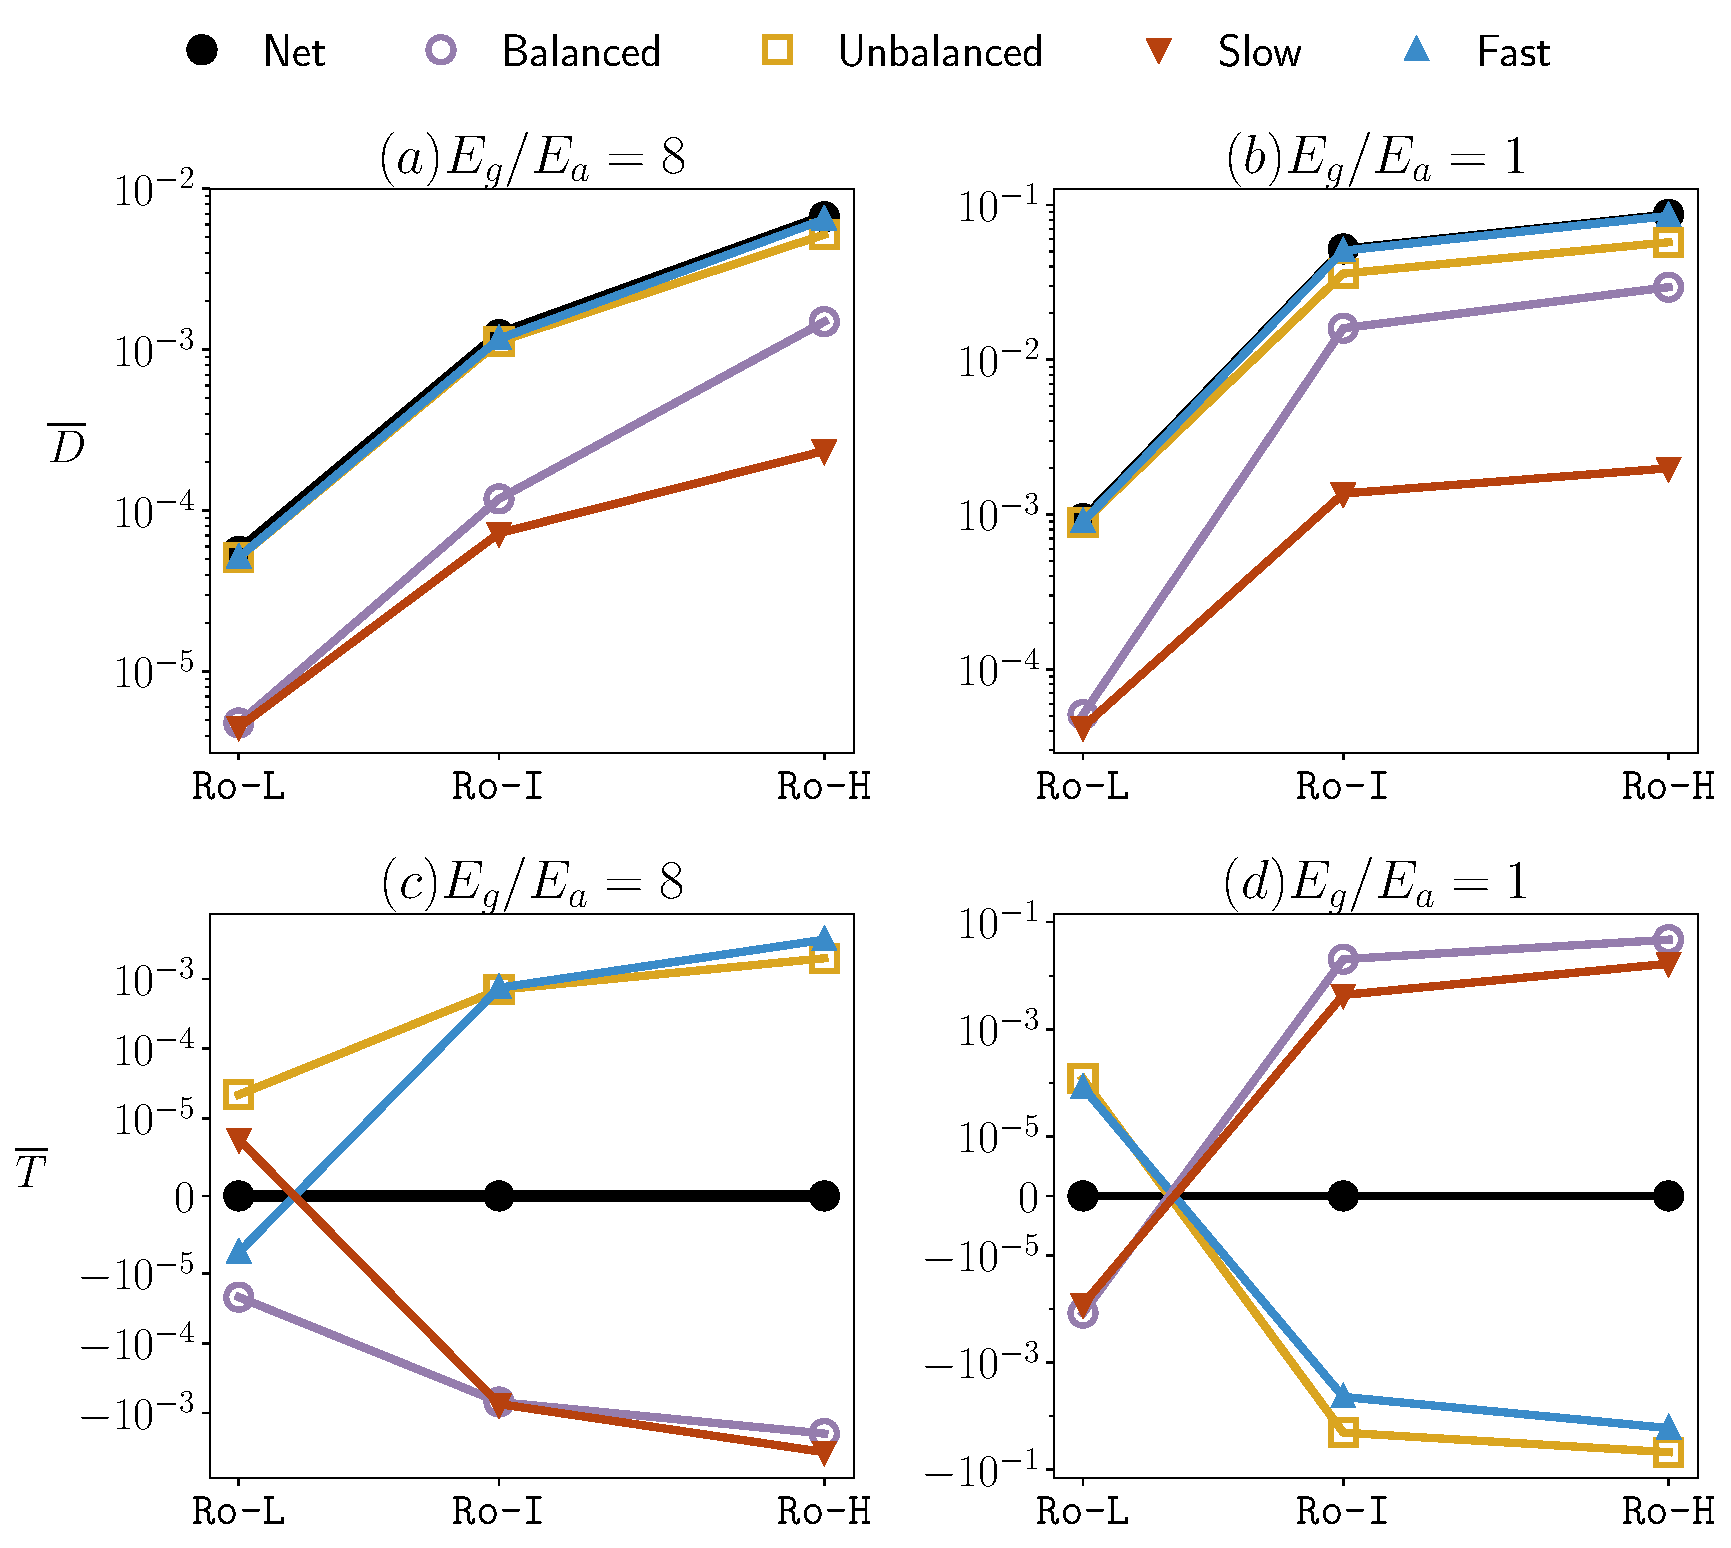
\includegraphics[width=1\linewidth]{./figures/internal_tide_eddy/tranfer_dissipation_net.pdf}
	\caption[Dissipation and nonlinear energy transfer between flow components]{ Dissipation (top row) and nonlinear energy transfers (bottom row) of the net flow and its different components. The dissipation and transfer for $E_g/E_a = 8$ flows (left column) are small compared to that of $E_g/E_a = 1$ flows (right column). The net flow dissipation (in black) increases with Rossby number and mostly comes from the fast component, while the ageostrophic dissipation comes close. The nonlinear transfer between the components is equal and opposite, and increases for intermediate (\ir) and high (\hr) Rossby number flows. The sign of nonlinear transfer between components changes between $E_g/E_a = 8$ (panel c) and $E_g/E_a = 1$ (panel d) flows, signifying that the direction of the energy transfer depends on the ageostrophic flow energy level.}
	\label{edwv-dt}
\end{figure}


 
Although the net flow can only gain energy through forcing and lose energy through dissipation, the individual flow components can act as each other's energy sources and sinks. For any flow component indicated with subscript $i$, this is measured by the energy transfer rate $T_i$ which is the flux at the zeroth mode, $\hat{\Pi}_i(0) = \sum_{s = 0}^{k_m} \hat{T}(s,t)$.  Since the nonlinear interactions conserve energy, the energy transfer rate of all the components adds up to zero. In other words, $\bar{T}_s + \bar{T}_f=0$ and $\bar{T}_g + \bar{T}_a=0$.  Panels (c) and (d) of Fig. \ref{edwv-dt} show the time-averaged energy transfer of different flow components across Rossby numbers for the $E_g/ E_a=8$ and $1$ flows, respectively. As mentioned above, $\bar{T}_s = - \bar{T}_f$,  $\bar{T}_g = -\bar{T}_a$, and the net transfer in black is zero. Looking at these panels, we see an increase in energy transfer rate of all components with Rossby number, and with ageostrophic energy $E_a$. From negligible values at low Rossby numbers, the transfer increases by orders of magnitude at intermediate and high Rossby numbers. The direction of energy transfer also changes based on $E_g/E_a$ values. For panel (c) with $E_g/E_a = 8$ flows, at intermediate and high Rossby numbers, the weak fast and the ageostrophic components extract energy out of the stronger slow and geostrophic components, respectively. However, in panel (d), for $E_g/E_a = 1$ flows with comparable geostrophic-ageostrophic and slow-fast energies, the ageostrophic and the fast components strengthen the geostrophic and the slow components, respectively. Surprisingly, despite their failure at capturing large-scale coherent structures at intermediate and high Rossby numbers, the energy transfer of geostrophic-ageostrophic decomposition is similar to that of the slow-fast decomposition, with comparable magnitude and the same direction of transfer for both $E_g/E_a =8$ and $E_g/E_a = 1$ flows.

The flows with different $E_g/E_a$ are further different when we compare their slow-fast transfer rate with the net dissipation. The eighth column of table \ref{edwv-t1} shows the magnitude of the slow-fast transfer to the net dissipation ratio. We see that for $E_g/E_a = 1$ flows, the slow-fast transfer rates are an order of magnitude weaker than the net flow dissipation. This is true across low, intermediate, and high Rossby numbers. This means that although the slow-fast transfer for such flows increases with Rossby number, the net dissipation rate caused by the forward cascade of energy increases accordingly. Contrast this with the $E_g/E_a= 8$ flows' slow-fast transfer to dissipation ratios in table \ref{edwv-t1}. While the slow-fast transfer is still small compared to the flow dissipation for \lre flow, it increases for \ire and \hre flows, and becomes comparable to the net dissipation.  Thus, for flows with weak ageostrophic energy, the slow-fast transfer at intermediate and high Rossby numbers transfers energy to the fast component and then cascades to small dissipative scales. On the other hand, for flows with comparable geostrophic-ageostrophic energy, the energy lost by the fast component to the slow component is minimal compared to their forward energy cascade that leads to dissipation. 

%\textbf{start here} 

%Note that these transfers are the not scale-wise energy transfer. That involves a more detailed analysis to uncover cross-component transfer across scales \citep{TD20,delpech_etal_2024,rajpoot2026}.


We note that the above discussion involved net transfers of fast and ageostrophic and slow and balanced components. Further dissection of the transfers and  flux into individual triadic components is something that is done in several previous studies \citep{RT26, delpech_etal_2024, TD20}. Such triadic interaction analysis needs much more data storage and is something we hope to undertake in the near-future. 

 
\section{ Frequency broadening and the  internal wave continuum } \label{edwv-fspectr}


	
	
In this section, we will explore the frequency spectrum and its features across the different flow regimes.     Figure \ref{edwv-iwc} shows the frequency spectra for flows with $E_g/E_a = 8$ and $E_g/E_a = 1$, in panels (a) and (b), respectively. For all Rossby numbers and $E_g/E_a$ ratios, the spectra show a peak at the nondimensional tidal forcing frequency, $\omega_0 = 1.73$. We see that the spectra drops to the left of the forced frequency, before rising again, and plateauing at the smallest frequency. This energy at low frequencies corresponds to the slowly evolving coherent eddies whose physical structures were discussed in \S \ref{edwv-ps}.
	
	
	 
	
	
	\begin{figure}
		\centering
		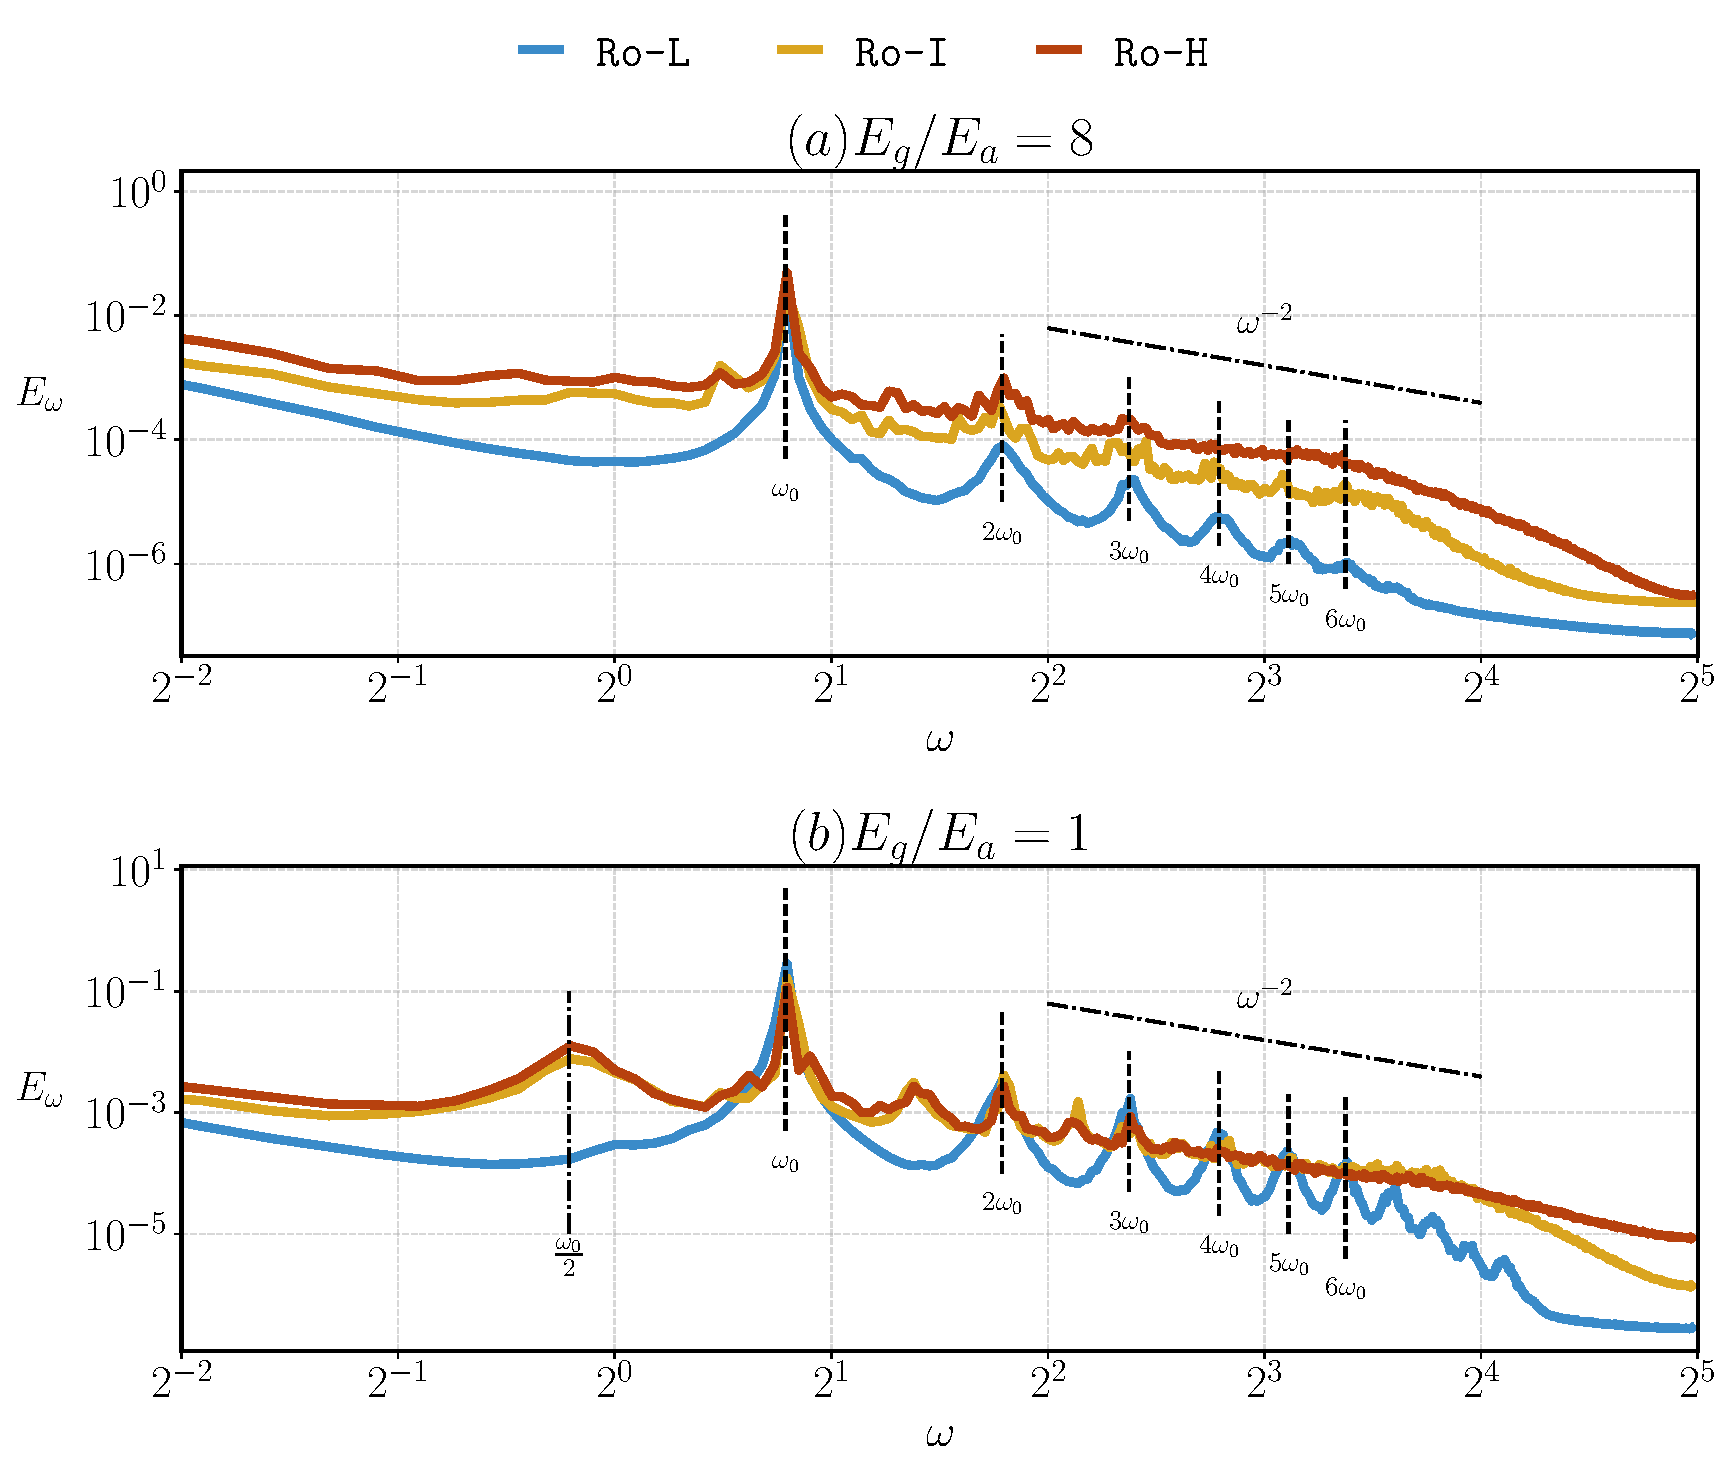
\includegraphics[width=1\linewidth]{./figures/internal_tide_eddy/frequencies.pdf}
		\caption[Frequency spectra and the formation of internal wave continuum]{ Frequency spectra for low, intermediate, and high Rossby number flows. Both the $E_g/E_a = 8$ flow (top row) and $E_g/E_a = 1$ flow (bottom row) form a continuum for intermediate and high Rossby numbers. Notice the prominent peak at the forced frequency, $\omega_0$, in all the spectra. The low Rossby number flows (\lr) only show peaks of tidal harmonics, which is insufficient to form an internal wave continuum. The dashed line corresponding to $\omega^{-2}$ is close to the slope of the continuum for \ir and \hr flows. }
		\label{edwv-iwc}
	\end{figure}
	
	

For the low Rossby number flows \lre and \lro, the blue-colored frequency spectra in Fig. \ref{edwv-iwc}(a,b) shows a peak at $\omega_0$, and at its higher harmonics labeled using dashed vertical lines. Nonlinear tide-tide interactions are known to generate such harmonics: see, for example, similar frequency spectra in Fig. 6 of \citet{buijsman2025} and \citet{hiron2025} and Figs. 4 and 5 of \citet{rolland2025}. These low Rossby number spectra are also steeper than $\omega^{-2}$ with no clear broadening or continuum formation. With increasing Rossby number, we see much broader high frequency spectrum. The discrete   frequency harmonics' peaks are more leveled off and the spectrum approaches a `continuum' of frequencies. This can be seen in the frequency spectra for intermediate and high Rossby number flows, \ir, and \hr, shown in yellow and red in Fig. \ref{edwv-iwc}(a,b), respectively, which resembles  a continuum for frequencies beyond the forcing frequency, with a slope close to $-2$. In general, a broadband frequency spectrum with slope close to $-2$ generated from    nonlinear interactions involving waves  is called a GM-like spectrum or IWC \citep{BWM17,chen2019,nelson2020,delpech_etal_2024}. We follow the same terminology and identify the high frequency broadband spectra with slope close to $-2$ as IWC.  From above, recall that nonlinear interactions increase significantly for \ir and \hr flows. These interactions play a role in the formation of the continuum. The nonlinear transfers for \lr flows, being significantly smaller, does not lead to a continuum.   Both $E_g/E_a = 8$, and $E_g/E_a = 1$ flows show this frequency broadening, but the continuum for the $E_g/E_a = 8$ flows in Fig. \ref{edwv-iwc}(a) falls off early, around $\omega = 10$, whereas it continues beyond $\omega = 16$ for $E_g/E_a = 1$ flows in Fig. \ref{edwv-iwc}(b). Therefore, increasing the ageostrophic energy level can further broaden the frequency spectra.   Note that while our results point out that strong nonlinearity facilitates the formation of the continuum, identifying  the specific frequency triads of the different flow components that facilitates the formation of the continuum   needs further exhaustive analysis, going beyond our present investigation. % and is not attempted here.
 
 
 %At this point 	it is worth noting that the difference between a broadband frequency spectrum and an internal wave continuum is subtle. A broadband frequency spectra with slope close to $-2$, generated from wave and eddy forcing is called GM-like spectrum \citep{BWM17,chen2019,nelson2020,delpech_etal_2024}. Some studies investigate the energy distributed in the frequency-wavenumber space like we did \citep{Muller_etal_2015,Pan_etal_2020,Yang_etal_2023, Ansong_etal_2024}. So far, for such mesoscale studies, energy lies around the dispersion lines that linear waves folloew. Thus, the continuum that forms in these studies are indeed internal wave continuum.
 	
    
Towards the low frequency end of the spectrum, in Fig. \ref{edwv-iwc}(b) for \hro and \iro flows, notice the small peak to the left of the forcing frequency. This frequency peak arises at one-half of the tidal forcing frequency, as highlighted with the dashed vertical line at $\omega_0/2$ in the figure. This feature is reminiscent of the parametric subharmonic instability that generates one-half the tidal frequency due to resonances, as shown in multiple past studies \citep{MacKinnon_Winters_2005, chen2019,wang2024}. However, interestingly, the frequency of this peak is less than the Coriolis frequency $\omega = 1$, the lower limit of wave frequency.  Doppler shifting of the waves by the underlying currents can generate frequencies less than the inertial frequency, and we speculate that the  $\omega_0/2$ frequency is  generated through a PSI-like mechanism in combination with Doppler shifting  \citep{shakespeare2020}.

Formation of a broadband continuum of frequencies  and its absence have been explored in different past studies. Multiple studies using simulations and observations have found that flows with tides, but without NIWs, primarily generate steeper frequency spectra with peaks at tidal harmonics \citep{rolland2025,hiron2025}, similar to the spectra seen in the low Rossby number cases in Fig. \ref{edwv-iwc}. \citet{sugiyama2009} forced tides and NIWs to obtain an IWC on a longer timescale in a two-dimensional vertical plane domain. Resolving submesoscales, \citet{Yang_etal_2023} showed that eddies can interact with NIWs, in the absence of tides, and form a broadband spectrum with a slope close to $-2$. Many of these past studies emphasize the need for NIWs' presence  to generate a broadband continuum. An exception has been in the presence of topography; tides alone have been shown to form IWC in the presence of rough topography \citep{chen2019}. Adding to the collection of studies that have found a broadband frequency spectra in different settings, here we find that tides at high Rossby numbers can interact with eddy fields and create a broadband continuum, in the absence of topographic features and NIWs. %How energy flows from the harmonics to the surrounding frequencies at intermediate and high Rossby number requires an energy-budget analysis in the frequency space. This requires computation and storage beyond our current capabilities. However, this is an important question that we aim to answer in the future.
	
	\begin{figure}
		\centering
		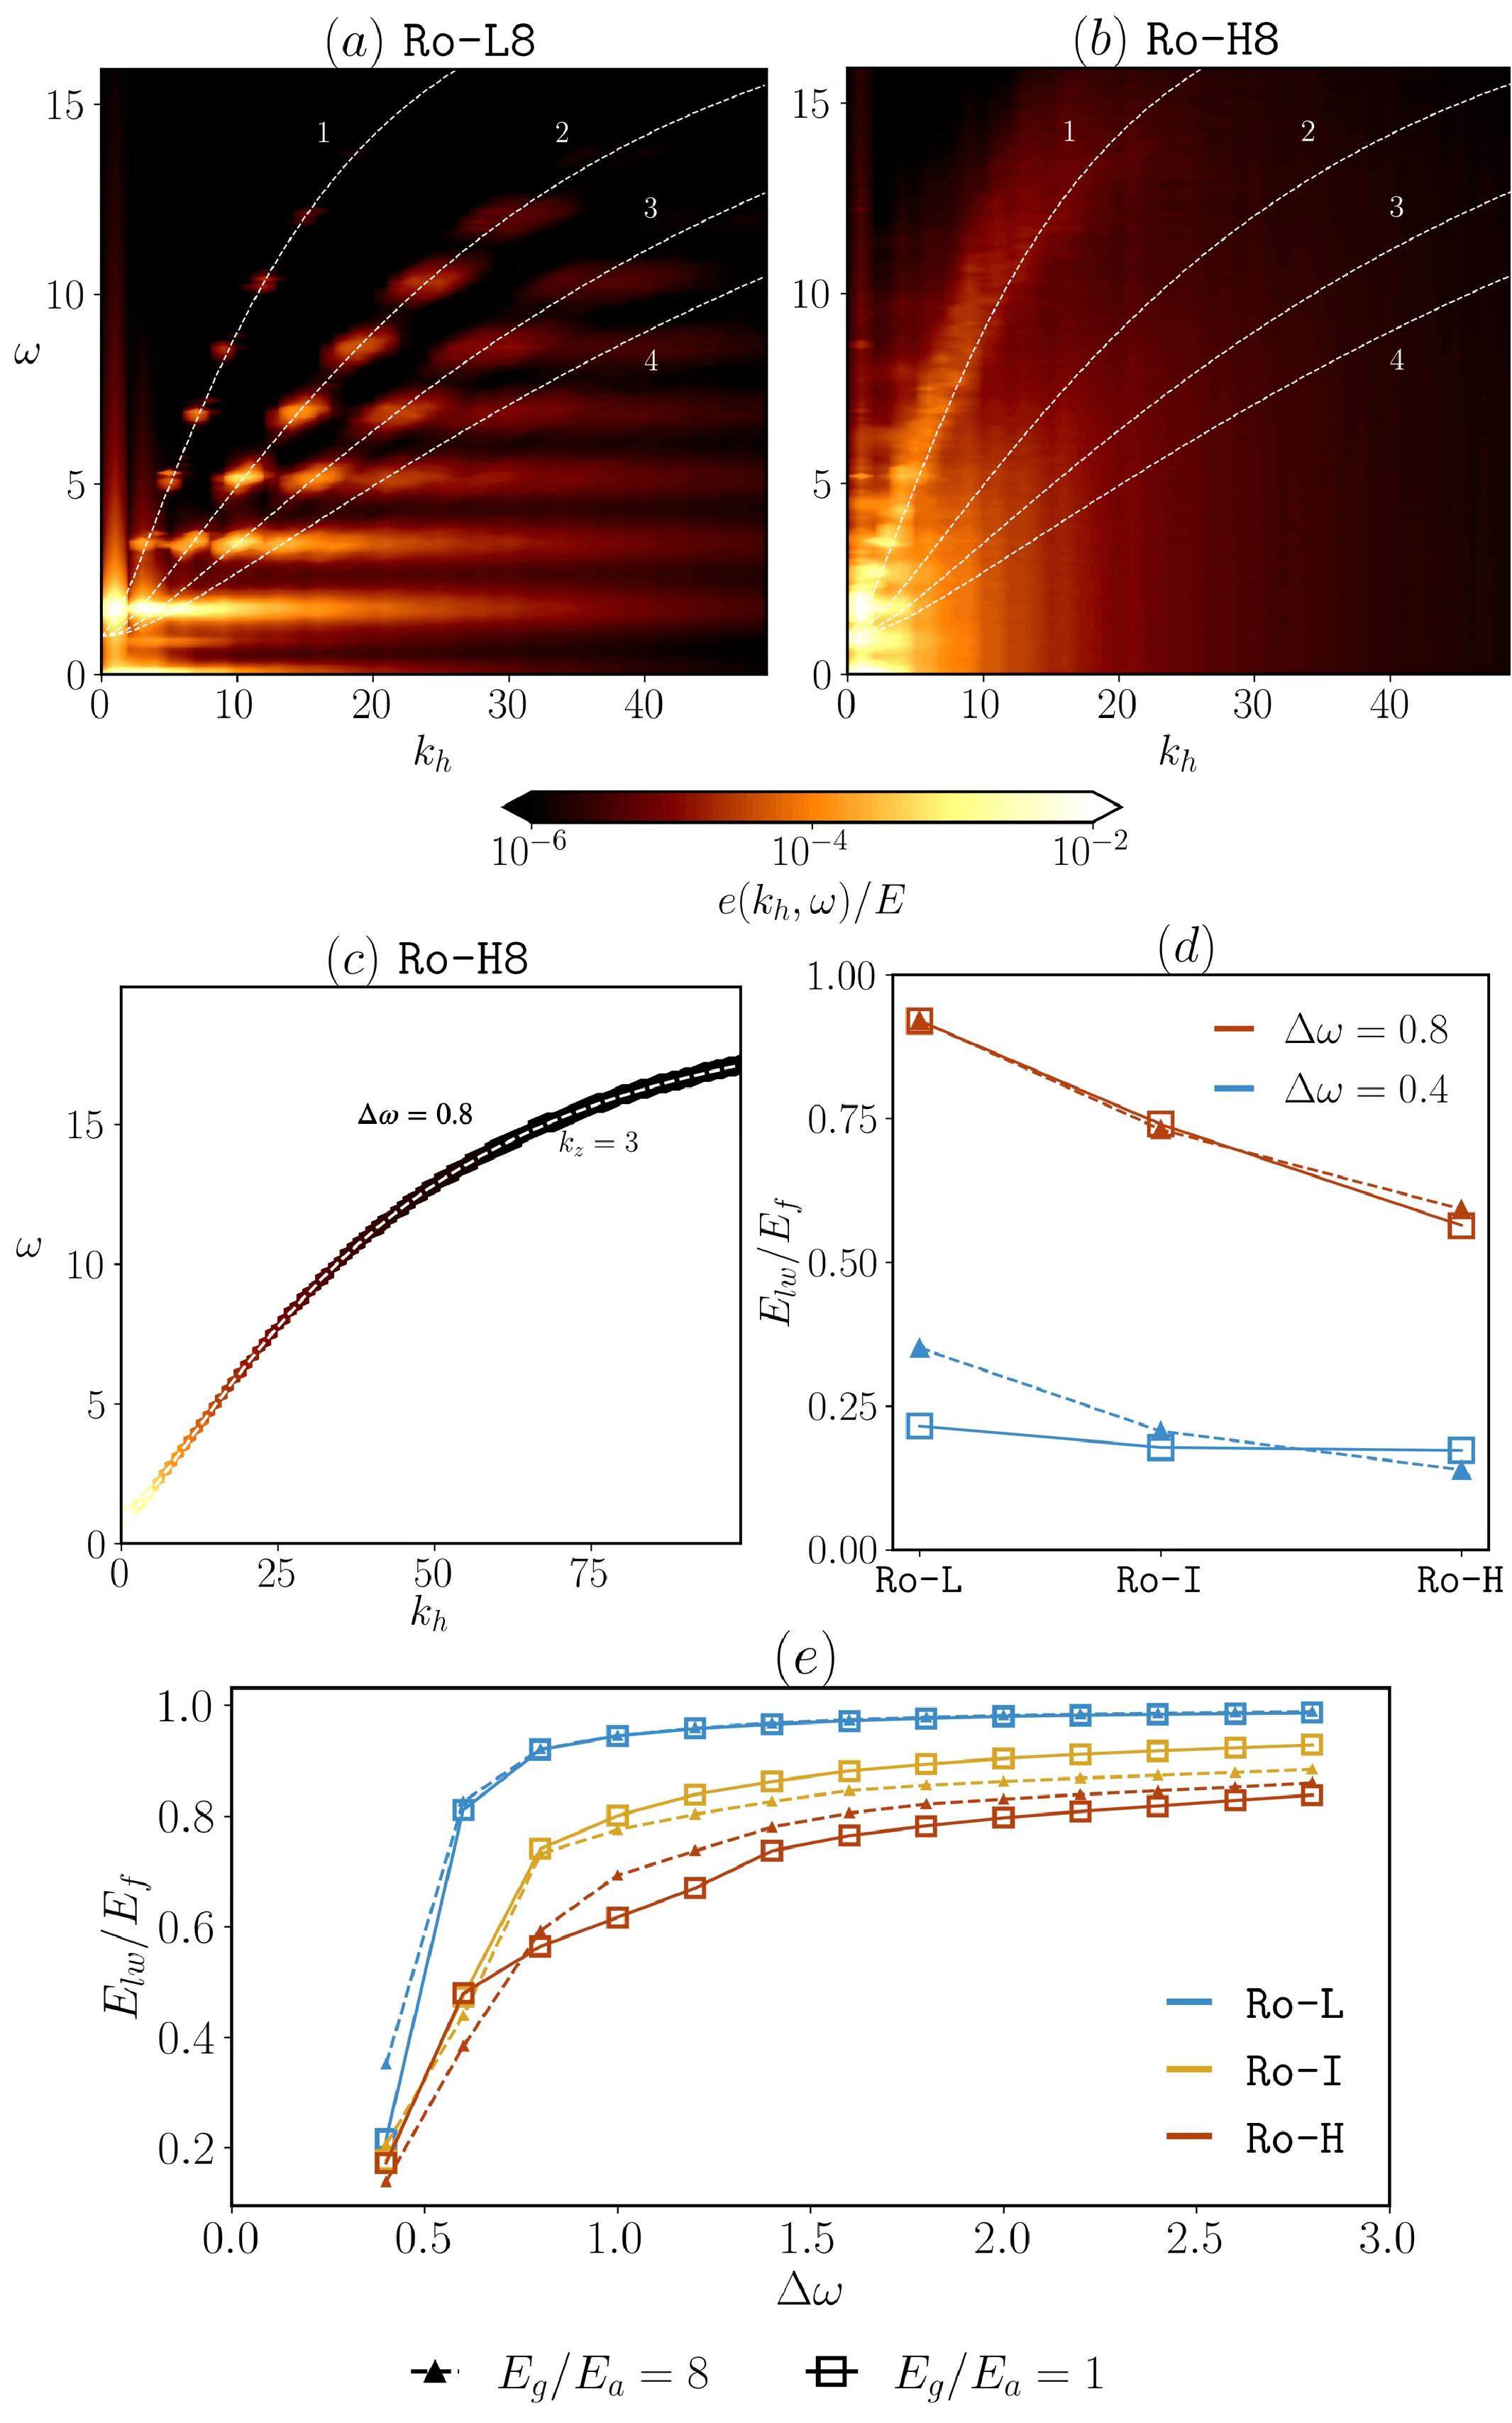
\includegraphics[width=0.75\linewidth]{./figures/internal_tide_eddy/omg_kh_linear_waves.pdf}
		\caption[Flow energy in the $\omega$-$k_h$ plane and the linear dispersive wave fraction]{ Flow energy plotted on the $\omega-k_h$ plane for \lre (a) and \hre (b) flows. Dispersion curves for different $k_z$ are denoted by broken white lines. Most of the energy is around the dispersion line for \lre flow shown in panel (a), indicating dominance of the linear waves. For high Rossby \hre flow shown in panel (b), energy is broadly distributed across the plane, indicating that a significant amount of fast energy is in flow components other than linear waves. Panel (d) shows fraction of linear wave energy as a function of Rossby number while panel (e) shows the fraction as a function of $\Delta \omega$. } %We calculate the linear wave energy by considering energy $\Delta \omega = 0.8$ width around the dispersion lines (c). The ratio of linear wave to fast energy, $E_w$, decreases for larger Rossby number flows (d). This is true across multiple values of $\Delta \omega$, and $E_g/E_a$ values (e). }
		\label{edwv-lwfrc}
	\end{figure}
	
	
	
	
	
	
    Although we see the formation of a broadband high frequency spectrum, the contribution of waves to the spectrum is unclear. % it is not clear if it is made up of dispersive internal waves. If it is, then the continuum is an IWC. 
    Specifically, it is useful to know what fraction of continuum comes from the dispersive waves. To find the contribution  of linear waves, we implement an extra decomposition here. We take Fourier transforms along all three spatial dimensions and time and integrate over angles in the horizontal wavenumber space $(k_x, k_y)$ to get the wavenumber-frequency spectral distribution of flow energy: $\hat{E}(k_h,k_z,\omega)$. Figures \ref{edwv-lwfrc}(a,b) show example horizontal distributions, $\hat{E}\left( k_h,\omega \right) = \sum_{k_z}\hat{E}(k_h,k_z,\omega)$, for \lre and \hre flows respectively. In Fig. \ref{edwv-lwfrc}(a) for \lre flow, many of the high-energy regions lie around the dispersion lines, signifying the dominance of linear waves in the system. Additionally, notice the prominent horizontal bands of energy along different $\omega$ values, which correspond to the tidal harmonics seen in Fig. \ref{edwv-iwc}(a). We also see high-energy regions close to $\omega=0$, corresponding to slowly evolving eddies. Similar horizontal bands of frequencies and dominant energy distribution around dispersion lines have been noted in previous studies, such as \citet{Ansong_etal_2024} and \citet{buijsman2025} in their Fig. 8, for example. These works used more realistic models (MITgcm and HYCOM), although their work, along with ours, shows a robust presence of linear waves and tidal harmonics in small Rossby number flows energized with internal tides. In contrast to the low Rossby number case, Fig. \ref{edwv-lwfrc}(b) for \hre flow shows energy more evenly distributed across the $\omega-k_h$ plane. This tells us that ageostrophic high-frequency flows, which do not follow the dispersion lines, contribute  to the flow  energy. 
    
    We calculated the amount of linear wave energy in each $k_z$ slice of $\hat{E}(k_h,k_z,\omega)$ in the neighborhood of the dispersion line of that particular $k_z$. An example of this is shown in Fig. \ref{edwv-lwfrc}(c) for the slice with $k_z = 3$. The sum of such energies from all the $k_z$ slices is the total energy coming from the linear waves. The ratio of the linear wave energy and the net fast energy indicates  the contribution of  linear waves in the flow spectrum. However, the width of the considered region around the dispersion line, $\Delta \omega$, is a free parameter. The $\Delta \omega$ shown in Fig. \ref{edwv-lwfrc}(c) is $0.8$. Changing $\Delta \omega$ changes the amount of  linear wave energy calculated in the system. The ratio of linear energy $E_{lw}$ to the fast energy $E_f$ is plotted as a function of Rossby number for two different values of $\Delta \omega$ in Fig. \ref{edwv-lwfrc}(d). We see that close to $90\%$ of the fast energy in \lre and \lro flows comes from the linear waves for $\Delta \omega = 0.8$. This means that at small Rossby numbers, the tidal harmonics in Fig. \ref{edwv-iwc}(a,b) formed due to the tide-tide interactions are mostly linear waves. For \ir and \hr flows with intermediate and high Rossby numbers, linear wave fraction falls to a little over $0.5$ for $\Delta\omega = 0.8$. This means that only about 50\% of the fast flow forming the continuum is made up of linear waves. 
    
    The same qualitative trend mentioned  above holds  for $\Delta \omega = 0.4$, although the fraction of linear waves further decreases. %The results for $\Delta \omega = 0.4$  show the similar trend across Rossby numbers. 
    Despite this, it must be noted that  $\Delta \omega = 0.8$ and  $\Delta \omega = 0.4$ are very narrow windows across dispersion curves. As seen from Fig. \ref{edwv-lwfrc}(c), $\Delta \omega = 0.8$ contains only a few pixels across the dispersion curves. We found the window $\Delta \omega = 0.4$ to be much more stringent, almost touching the dispersion curves  due to the low number of pixels in frequency-wavenumber space that this window contains (figure omitted).  %  only contains two points or pixels along $\omega$ in the $\omega - k_h$ plane. Therefore, it is an inadequate threshold to capture small spreads along the dispersion lines. Thus, 
    Consequently,  we focus on the estimates from   $\Delta \omega = 0.8$, a more realistic threshold. For this threshold, linear waves hold more than 50\% energy of the fast motions at all Rossby numbers. In general, for fixed $\Delta\omega$ $E_{lw}$ decreases with increasing Rossby numbers for both $E_g/E_a = 8$ and $E_g/E_a = 1$ flows.
       
  %    Consequently, such small windows capture only the energy in the immediate vicinity of the dispersion curves and would miss nonlinearity induced spreading of wave energy.  
  %  Of course, $\Delta\omega$ is a variable and the linear wave fraction can change based on this variable, as seen 
    
    Further increasing the window width, we see from  Fig. \ref{edwv-lwfrc}(e) that $E_{lw}$ increases monotonically with $\Delta\omega$ for all Rossby numbers and all energy ratios. More than 80\% linear wave fraction is attained even for high Rossby number flows when $\Delta\omega$ exceeds 2.5. However, such a high $\Delta\omega$ brings in energy from flow components scattered further away from the dispersion curves. If we keep $\Delta\omega$ fixed at 0.8, which leads to a reasonably narrow window   around the dispersion curves, as seen in Fig. \ref{edwv-lwfrc}(c), about 90\% of the fast energy comes from linear waves at low Rossby numbers, while only about 50\% of fast energy is from linear waves at high Rossby numbers. 
       
    The above feature is in some sense expected, since with increasing Rossby number, stronger nonlinear interactions and scattering of waves by eddies and other waves are prominent, spreading wave energy more broadly across the dispersion curves. Since more than 50\% of the energy comes from linear waves, and since nonlinear broadening of energy across dispersion curves is expected in high Rossby number flows, we still identify the high frequency broadband spectrum as internal wave continuum.  This terminology also aligns with the usage that is prevalent in the oceanographic community, although it must be kept in mind that  the fast flow component that makes up the IWC is not localized along dispersion curves, but rather  has some non-negligible distribution of energy across the dispersion curves. 
    
    
    
    
    
  %  However, the points made above reveal limitations in using linear wave theory for higher Rossby number frequency spectra. In other words, the broadband continuum in higher Rossby number flows will have non-negligible energy coming from fast components that do not follow the description of linear waves, and as a result, linear wave theory should be applied cautiously to such flows. Furthermore, Doppler shifting can alter the frequency of the linear waves, away from the dispersion lines which can alter the fraction of linear wave energy we find in Fig. \ref{edwv-lwfrc}(d). With these caveats noted, we still identify the high frequency broadband spectrum as internal wave continuum for multiple  reasons. One, the fraction of linear waves is more than 50\%, implying that linear waves have  a dominant contribution. Second, 
    
    
    %, one might wonder if it is approproate to call the high 
    
    
    %In the future, we will add similar diagnostics with Lagrangian particles to quantify the effect of Doppler shift across Rossby numbers.
	
\section{ Energy flux in physical space and turbulent cascade efficiency }\label{edwv-flux}
    
	
  
	While the spectral flux $\hat{\Pi}$ in \eqref{edwv-fxe} informed us about the rate of downscale energy transfers with increasing Rossby number, it lacks information on how different regions of the flow in physical space transfer energy. Here we will explore features of the energy flux in physical space with an eye on regions where the bulk of the energy transfer happens.  Examining the physical features of the energy flux can help us  understand the different mechanisms responsible for energy transfers across length scales \citep{Alexakis_Chibbaro_2020, Dubrulle_2019,johnson2021, TV22, delpech_etal_2024, THR26}. It can also be used to study how efficiently different length scales are involved in transferring energy across scales \citep{ballouz2018,johnson2021}. 
	
%	Such studies are common across the oceanographic and fluid dynamics community \cite{RP2006, Capet_etal_2008c, Groeskamp_etal_2017,srinivasan_etal_2023,delpech_etal_2024,barkan2024,gao2024, Bandi_etal_2006, Davidson_2008,ballouz2018, Dubrulle_2019, Alexakis_Chibbaro_2020, johnson2021}. Analysis of the different terms of the physical flux helps understand the different mechanisms responsible for energy transfers across length scales \cite{delpech_etal_2024,johnson2021}. It can also be used to show how efficiently different length scales are transferring energy across scales \cite{ballouz2018,johnson2021}. 
	
	To arrive at an expression for the energy flux in physical space at a particular length scale $\ell$, one needs to separate the flow into length scales smaller and larger than $\ell$. This is done by applying a spatial filter on the flow components that commutes with the space and time derivatives. Thus, the net flow components $\vec{v}, \ w$, and $b$ are separated into large-scale flows $\t{\vec{v}},\ \t{w}$, and $\t{b}$ and small-scale flows $\vec{v}', \ w'$, and $b'$ such that they add up to form the net flow. The length scale $\ell$ of the separation is specified by the filter. The pointwise energy of the large-scale flows can then be defined as 
    \begin{align}
    \label{edwv-flte}
    \begin{split}
        \t{e} = \frac{1}{2}\left( \t{u}^2 + \t{v}^2 + \frac{\t{w}^2}{\alpha^2 } + \t{b}^2 \right) \ .
    \end{split}
    \end{align}
 In the absence of forcing or dissipation, $\t{e}$ evolves in time according to 
    \begin{align}
        \label{edwv-ebdg}
        \begin{split}
            \Dp{\t{e}}{t}{} + \Sigma_\ell = - \Pi_\ell \ .
        \end{split}
    \end{align}
    
 Above $\Sigma_\ell$ is the sum of divergence terms and vanishes when integrated over the domain. $\Sigma_\ell$ therefore represents quantities that redistribute energy within the domain without transferring it across scales. $\Pi_\ell$, on the other hand, is the energy flux responsible for transferring energy across scales. A detailed derivation of the scale-wise energy equation \eqref{edwv-ebdg} for the Boussinesq equations is given in appendix \ref{edwv-fluxeqn}. The various terms take the form
     \begin{subequations}
        \begin{align}
            \label{edwv-pi}
            \Pi_\ell &= Ro\left[\uptau:\del\t{\vec{v}} + \vec{\tau}.\Dp{\t{\vec{v}}}{z}{} + \frac{1}{\alpha^2}\vec{\tau}.\del_3 \t{\vec{u}} + \vec{B}.\del_3\t{b}\right] 
        \end{align}
        \begin{align}
            \label{edwv-td}
            \Sigma_\ell &= Ro~\left[ \del_{3} .\left[\t{\vec{u}} \left(\t{e} + \frac{\t{p}}{Ro}\right) - \t{b} \vec{B}\right] - \left[\del.\left(\t{\vec{v}}.\uptau\right) + \Dp{}{z}{}\left(\t{\vec{v}}.\vec{\tau}_h\right) \right] - \frac{1}{\alpha^2}\del_3.\left(\t{w}\vec{\tau}\right)\right] \ ,
        \end{align}
    \end{subequations}
 where $\bs u =(u,v,w)$ is the three dimensional velocity vector, $\del_3 = \del + \hat{z} \partial/ \partial z$, is the three dimensional gradient operator, and 
    \begin{align}
        \begin{split}
            \uptau = \left[\begin{matrix}
                \t{u}^2 - \t{u^2} & \t{u}\t{v} - \t{uv}\\
                \t{u}\t{v} - \t{uv} & \t{v}^2 - \t{v^2}\\
            \end{matrix}\right] &\ , \ 
            \vec{\tau} = \left(\vec{\tau}_h , \t{w}^2 - \t{w^2}\right), \\ 
            \vec{\tau}_h = \left(\t{u}\t{w} - \t{uw},\t{v}\t{w} - \t{vw}\right) \ , \ \vec{B} &= \left(\t{u}\t{b} - \t{ub},\t{v}\t{b} - \t{vb},\t{w}\t{b} - \t{wb}\right) \ .
        \end{split}
    \end{align}
    
    
 Integrating \eqref{edwv-ebdg} over the domain gives us
    \begin{align}
        % \label{}
        \begin{split}
        \frac{d}{dt}\int_D \t{e} \ dx dy dz = -\int_D \Pi_\ell \ dx dy dz \ .
        \end{split}
    \end{align}
 If the domain integral of $\Pi_\ell$ takes a positive sign, large scales are losing energy to small scales, i.e., a forward energy cascade. We used a sharp wavenumber filter $k_\ell=2\pi/l$ in $k_h$ and $k_z$ separately to construct the flux in physical space. $k_\ell$ was chosen such that it lies in the inertial range for all the flows. 
	
	\begin{figure}
		\centering
		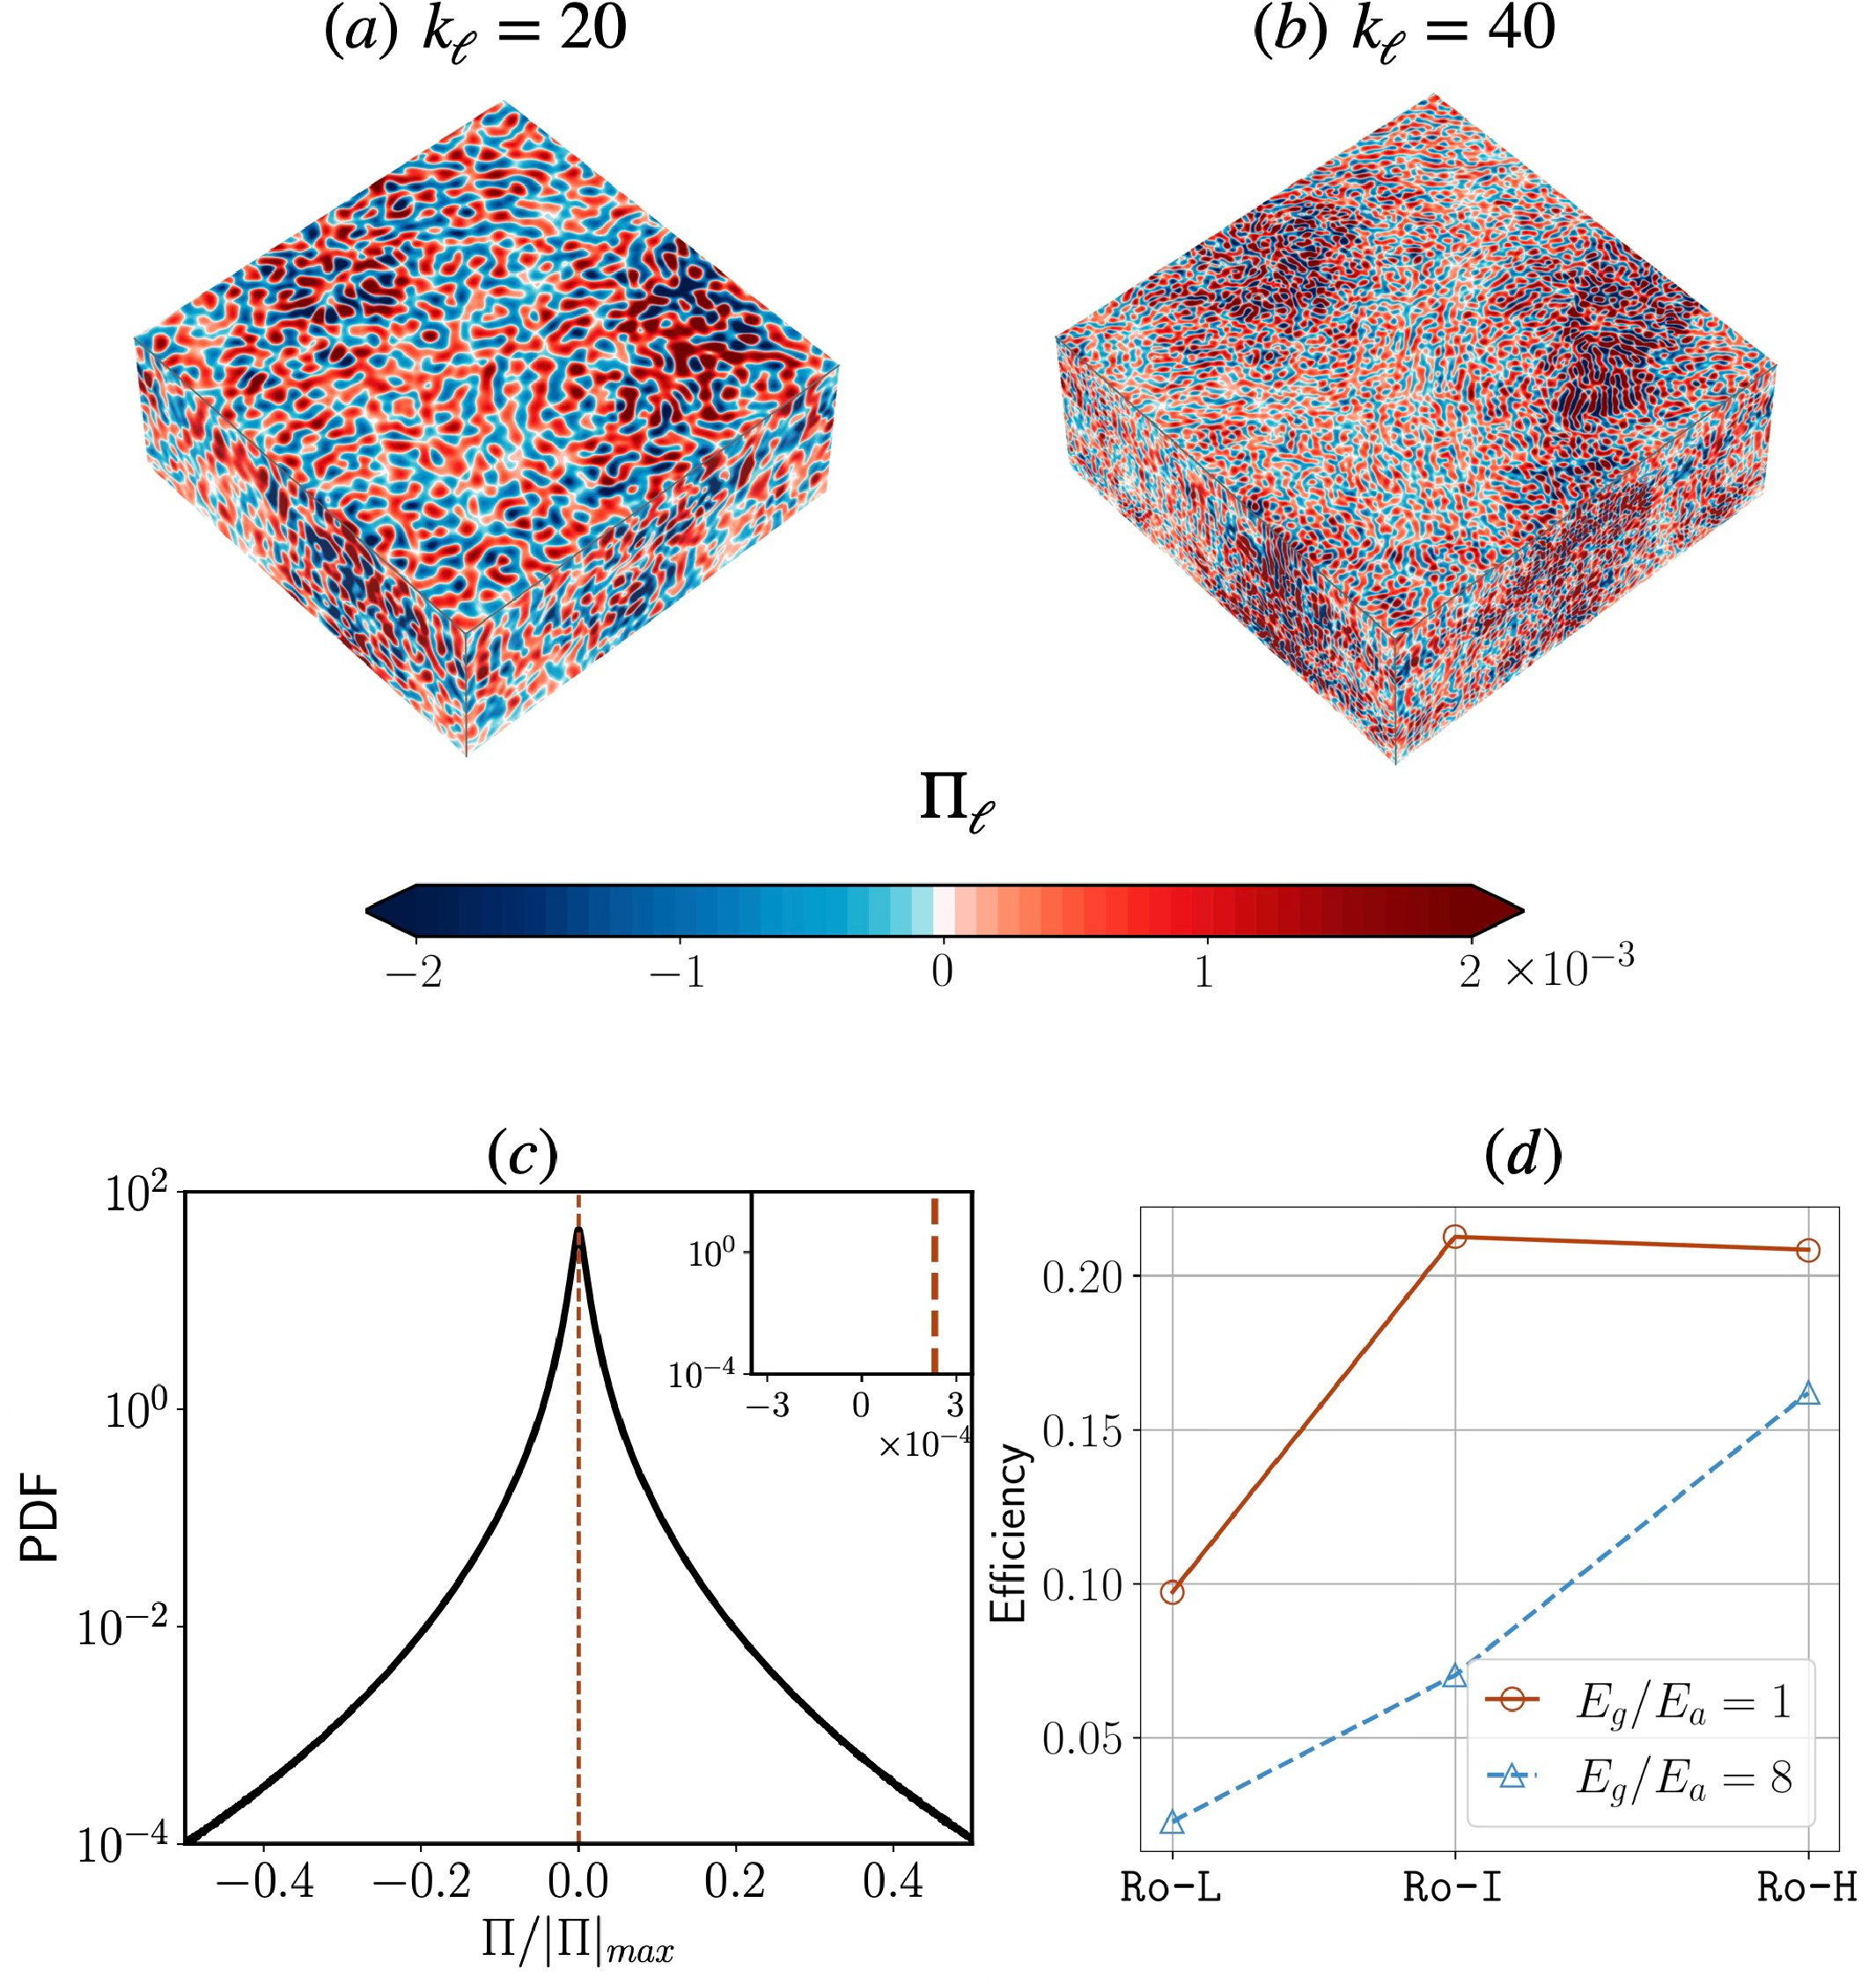
\includegraphics[width=1.0\linewidth]{./figures/internal_tide_eddy/flux-efficiency-structure-pdf.pdf}
		\caption[Structure and probability distribution of the physical flux and the cascade efficiency]{ Top row shows structure of physical flux $\Pi_\ell$ for two different filtering wavenumber $k_\ell = 20$ and $k_\ell = 40$ respectively. Observe that $\Pi_\ell$ can take pointwise positive or negative values across the domain and the size of the structures is inversely proportional to $k_\ell$. (c) PDF of the flux at $k_\ell = 40$. The mean is shown with the dashed vertical line, this being highlighted in the inset. (d) The cascade efficiency of flows increases with increasing Rossby number and ageostrophic flow energy.}
		\label{edwv-flxeff}
	\end{figure}
	
    The top row of Fig. \ref{edwv-flxeff} shows the physical flux of \ire flow for two filtering wavenumbers. Notice that the flux takes both positive and negative values across the domain. The physical structure of the flux also depends on the filtering length scale. That is why the structures in the flux for $k_\ell = 20$ in Fig. \ref{edwv-flxeff}(a) are bigger than the structures for $k_\ell = 40$ in Fig. \ref{edwv-flxeff}(b). However, at both length scales, the domain-integrated flux is positive, indicating a forward cascade. Figure \ref{edwv-flxeff}(c) shows the probability density function (PDF) of the flux at $k_\ell = 40$. The PDF has a slight asymmetry between the positive and the negative values, making the mean of the flux nonzero, as highlighted in the inset of Fig. \ref{edwv-flxeff}(c). Other flux PDFs were similar and are therefore omitted here. In the remainder of this section, we present results for $k_\ell = 40$, a filtering wavenumber that lies in the middle of the inertial range.
	
	
	\subsection{Efficiency of the turbulent cascade}
	
	A feature seen from the flux PDF in Fig. \ref{edwv-flxeff}(c) is that the mean is more than three orders of magnitude smaller than the extreme flux values. This is an indication of the inefficiency of the turbulent cascade: although high flux values would be seen in the physical domain, both positive and negative fluctuations arise, leading to significant cancellations in the net domain-integrated flux. We will now try to quantify the efficiency of the cascade. The energy budget equation in \eqref{edwv-ebdg} tells us that the nonlinear terms in the Boussinesq equations can either move energy around in the physical space using $\Sigma_\ell$, or transfer it across scales through $\Pi_\ell$. The ratio of the cross-scale energy transfer rate to the advected energy transfer rate, therefore, can tell us how efficient the flow is at transferring energy from one scale to another. 
    
    
    
 Notice that the sum of the divergence terms, $\Sigma_\ell$, in \eqref{edwv-td} contains a pressure term that is independent of Rossby number, like other linear terms in the Boussinesq equations \eqref{edwv-bsnq}, and does not vanish when we set $Ro = 0$. The remaining terms in \eqref{edwv-td} have explicit Rossby number dependence that comes from the nonlinear terms of \eqref{edwv-bsnq}. Furthermore, the spatial mean of $\Sigma_\ell$ in \eqref{edwv-td} is zero as it is made up of divergence terms. To calculate the efficiency of the turbulent cascade from nonlinear interactions, we took the ratio of the root-mean-square (RMS) of the flux, $\Pi_\ell$, and the divergence terms $\Sigma_\ell$ without the pressure term. This ratio measures the efficiency of the flow in transferring energy across scales with respect to advecting it within the domain. Note that, as there is no explicit Rossby number dependence in the ratio, it is not clear a priori how the efficiency should vary across  Rossby number. We also checked the efficiency by keeping the pressure term and found that it slightly decreased compared to the values shown below, specifically at low Rossby numbers. 

Figure \ref{edwv-flxeff}(d) shows that the efficiency of the turbulent cascade calculated, as described above, increases from low to high Rossby number flows. This indicates that \ir and \hr flows are more efficient at transferring energy across scales than low Rossby number \lr flows. The flow therefore has an increasing  tendency to transfer energy across scales rather than transferring it within the domain as   Rossby number increases. Additionally, $E_g/E_a = 1$ flows have more efficiency compared to the $E_g/E_a = 8$ flows across Rossby numbers. This means that ageostrophic flows not only increase the cross-scale energy transfer of the net flow, but also increase the general tendency of the flow for a downscale energy cascade. This was expected, as Figs. \ref{edwv-ekl} and \ref{edwv-eke} showed that the ageostrophic and the fast components dominated the positive flux of the net flow in the inertial range. Among all flows, the efficiency is maximum for \iro and \hro flows, and saturates around 20\%. 
    
    
 Despite the increase in efficiency with an increase in Rossby number and ageostrophic energy level, we see that the maximum efficiency is quite low, around 20\%. This reveals that the turbulent downscale cascade is relatively inefficient, with the flow moving more energy around the domain at a specific scale compared to transferring it across that scale. Similar results have been found in previous studies exploring three-dimensional homogeneous isotropic turbulence \citep{ballouz2018,johnson2021}. These studies report efficiencies below 40\%. Of course, they use different definitions of efficiency, involving relative alignments of vorticity and strain, making a direct comparison with our results difficult. Nevertheless, rotating stratified flows with fluctuating wave fields would be expected to be more inefficient than homogeneous isotropic turbulence, which is composed of strongly nonlinear vortical interactions. We will next explore physical space regions where the dominant share of the energy flux is located.
	
	\subsection{Physical regions contributing dominant share of flux}
	
	

	
    In the previous sections, we saw large-scale coherent eddies breaking up with increasing Rossby number, as a consequence of increasing forward energy flux. Vorticity, $\zeta$, is the standard variable we looked at to see large-scale eddy fields. On the other hand, horizontal divergence $\del \cdot \bs v$ is an indicator of ageostrophic flow components. Here we will explore the distribution of the physical flux with regard to vorticity and divergence. 
	
	\begin{figure}
		\centering
		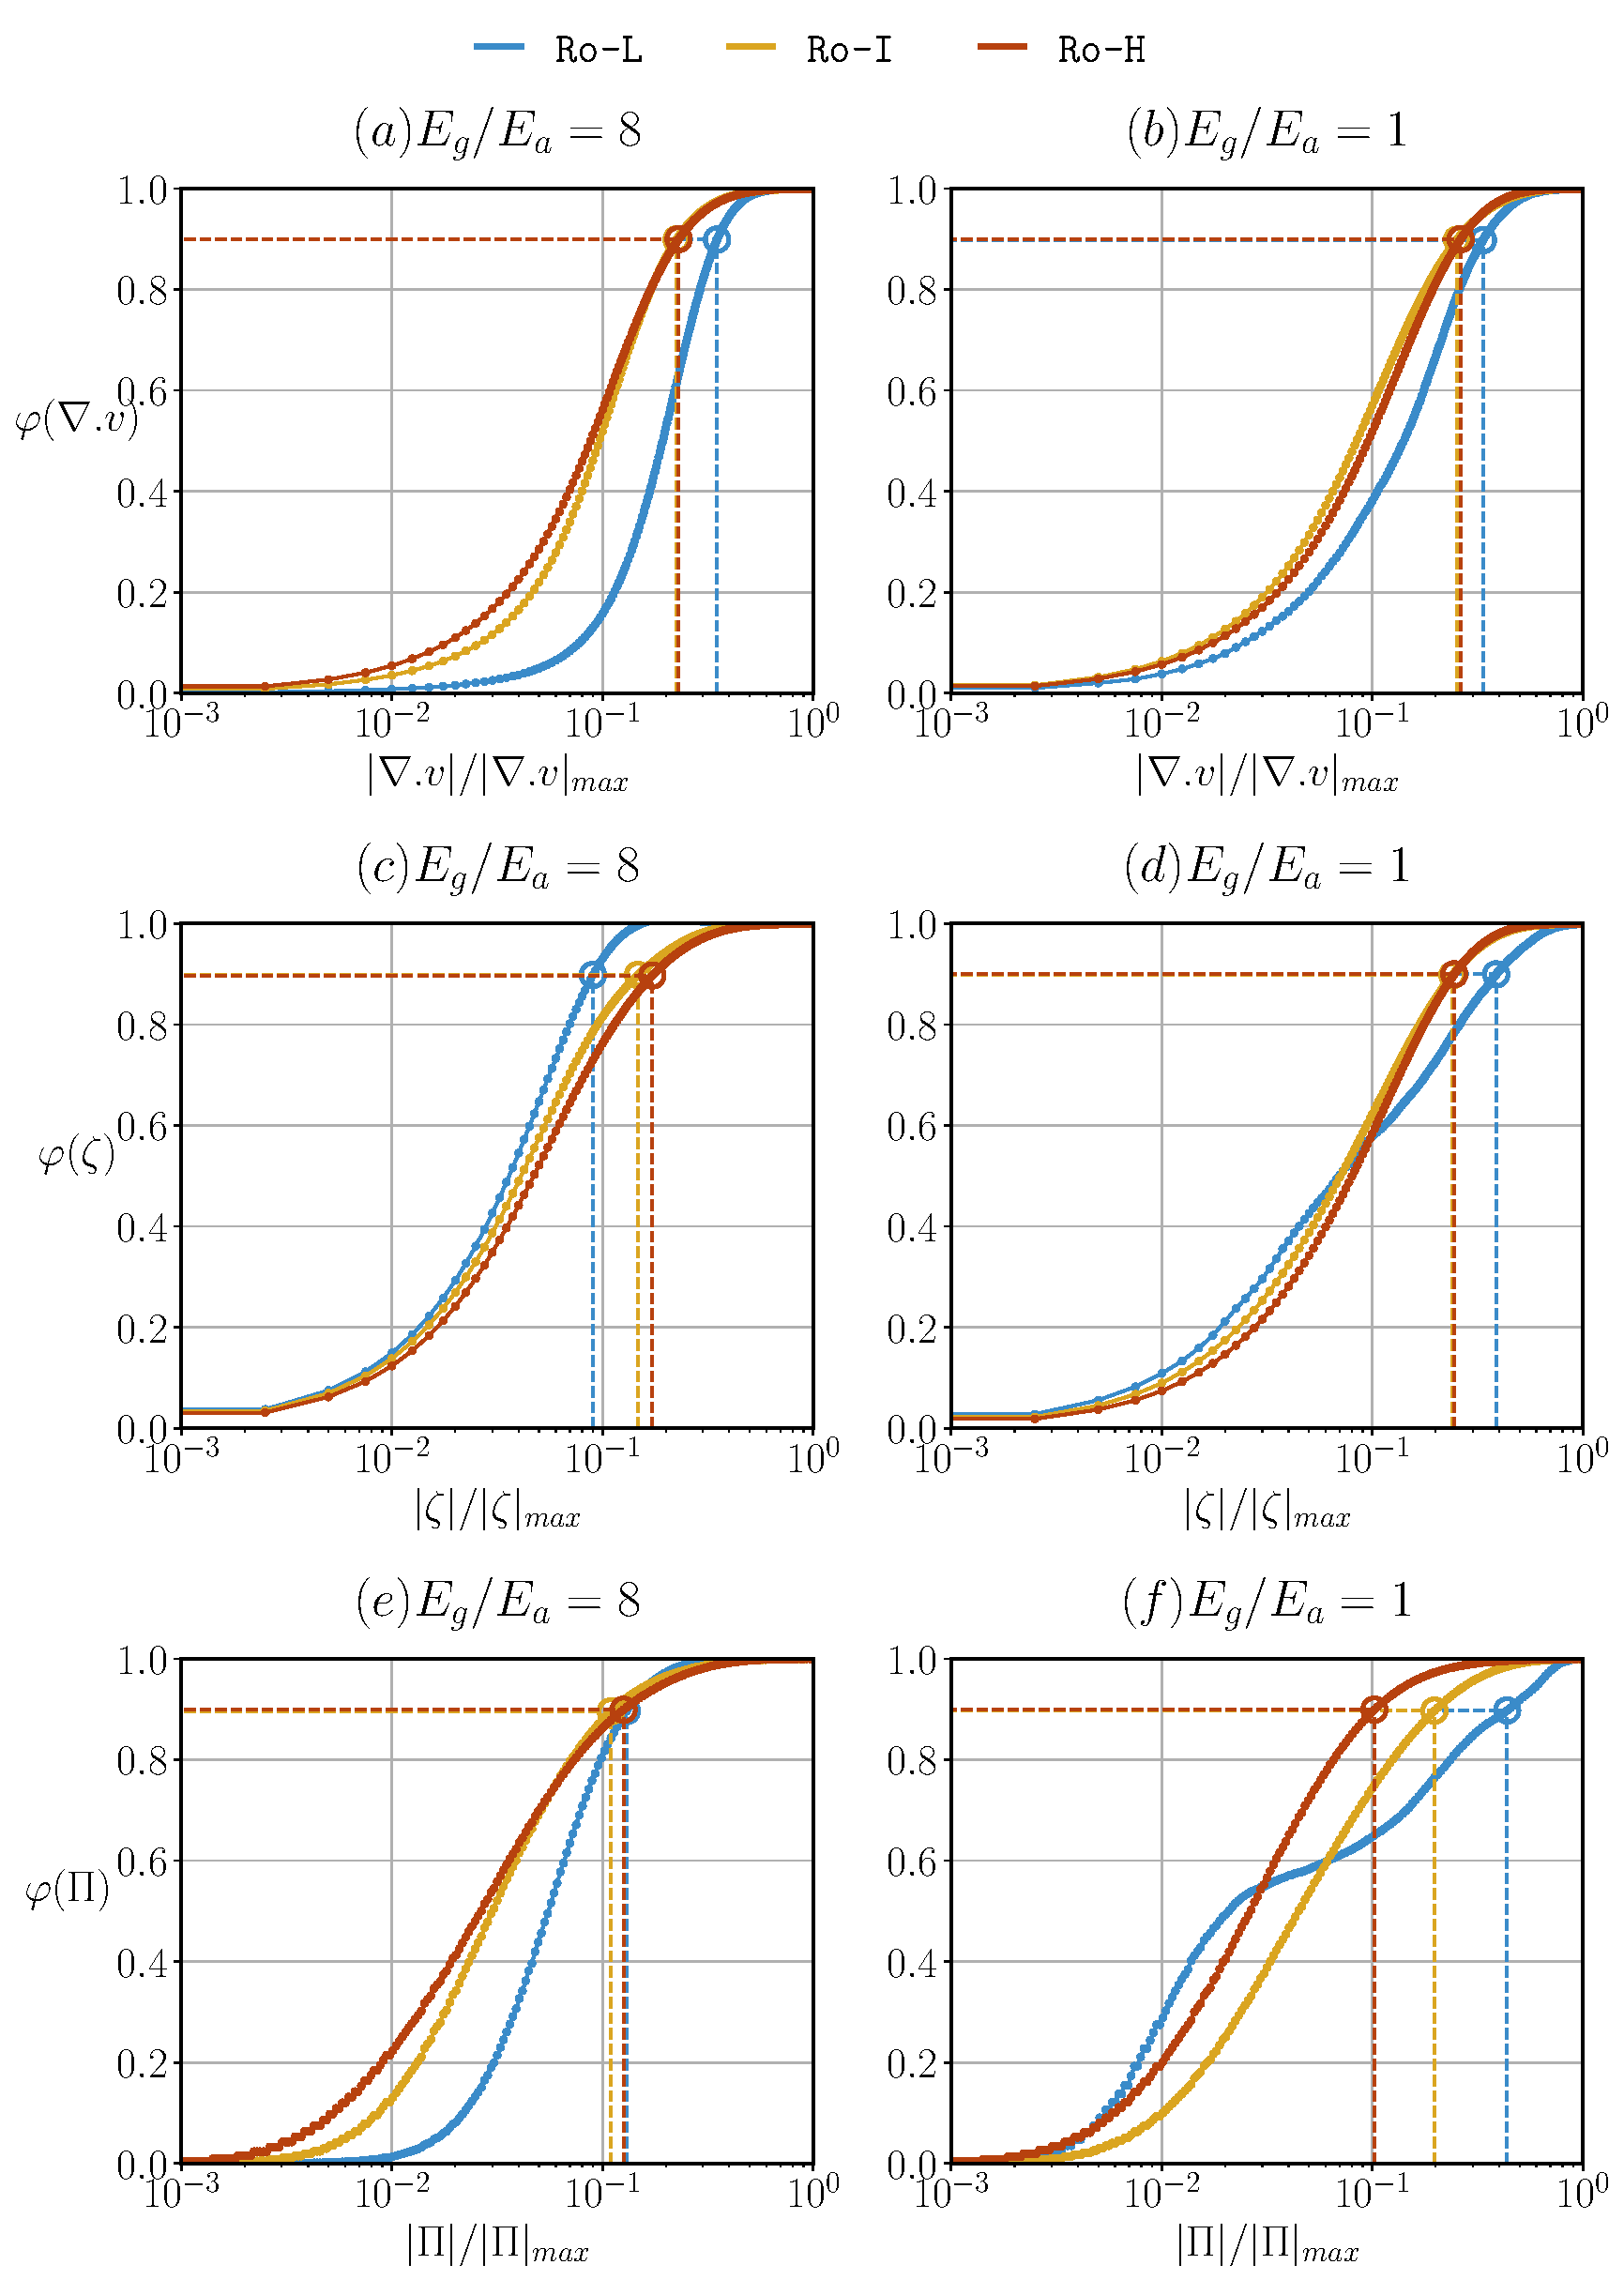
\includegraphics[width=0.9\linewidth]{./figures/internal_tide_eddy/normalized_flux_fracs.pdf}
		\caption[Flux fraction of horizontal divergence, relative vorticity, and filtered flux]{Flux fraction as a function of normalized horizontal divergence (top), relative vorticity (middle), and filtered flux (bottom) for $E_g/E_a = 1$ (left) and $E_g/E_a =8$ (right) case. Field values close to the maximum do not contribute much to the net flux, and the flux fraction saturates to $1$ well before the field values reach their maximum. The circles indicate 90\% of the flux fraction, and for all fields, it hovers around a tenth of the field maximum.}
		\label{edwv-flxfrc}
	\end{figure}
	
	
	
	Flow gradients make up the flux $\Pi_\ell$ in \eqref{edwv-pi}. Naturally, therefore, regions of extreme flow gradients will also have high flux magnitudes. However, the total integrated flux in these high gradient regions remains unclear. As discussed earlier, the flux PDF in Fig. \ref{edwv-flxeff}(c) shows that extreme flux values are orders of magnitude larger than the mean flux. Additionally, these extreme fluxes are very rare. To understand the distribution of flux with respect to flow strength, we plot the cumulative flux fraction $\varphi$, as a function of normalised absolute values of $\del \cdot \bs v$ and $\zeta$ in Figs. \ref{edwv-flxfrc}(a,b), and (c,d) respectively. Furthermore, to see how extreme fluxes contribute to the net flux, in Figs. \ref{edwv-flxfrc}(e,f), we plot the flux fraction $\varphi$ against the absolute value of the physical flux normalised by its maximum.
    
 For any field $\xi$, the cumulative flux fraction $\varphi(\xi_0)$ is calculated by integrating all the flux that lies in the region where $-\xi_0<\xi <\xi_0$, and dividing it by the total integrated flux. This is done for $\xi_0 \in [0, \op{max}|\xi|]$. For $\xi_0 = 0$, $\varphi = 0$, and for $\xi_0 = \op{max}|\xi|$, $\varphi = 1$. In Figs. \ref{edwv-flxfrc}(a,b), (c,d), and (e,f), $\xi$ are the three different fields: horizontal divergence $\del \cdot \bs v$, vorticity $\zeta$, and the physical flux $\Pi_\ell$. We see that in all the cases, regions close to the maximum values of the fields contribute very little to the integrated flux. For different Rossby numbers and $E_g/E_a$ values, the circles in Fig. \ref{edwv-flxfrc} are the points where $\varphi = 0.9$. This sets the thresholds for the three fields, which contain $90\%$ of the integrated flux. In fact, for all the Rossby numbers and the $E_g/E_a$ values, the flux fraction reaches $0.9$, close to $1/10$th of the maximum of all three fields. Figures \ref{edwv-flxfrc}(e,f) also tells us that regions having flux values close to the maximum contribute very little to the flux fraction. This is because regions with extreme horizontal divergence, vorticity, or flux are very rare in the domain. Although flux in such regions might be large compared to any other parts of the domain, their net contribution is low. 
	
	\begin{figure}
		\centering
		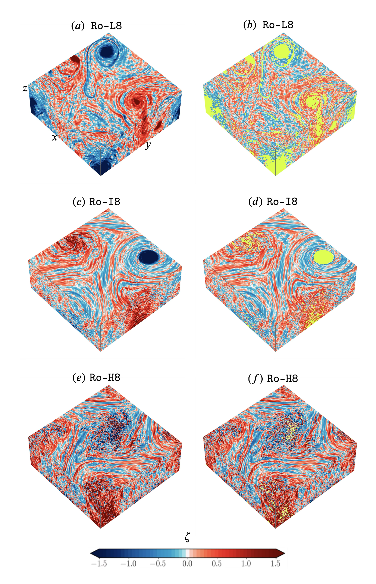
\includegraphics[width=0.8\linewidth]{./figures/internal_tide_eddy/0.9-flux-fraction-vorticity-structure-lw-3d.pdf}
		\caption[Vorticity regions holding $90\%$ of the integrated flux]{ Regions of vorticity containing $90\%$ of the integrated flux (right column), for $E_g/E_a = 8$ flows. Yellow regions are the high vorticity regions that contain the remaining $10\%$ of the flux. The Rossby number changes from low (\lre, top row), to intermediate (\ire, middle row), to high(\hre, bottom row). The vortex cores in the left column are absent in the filtered regions in the right column, signifying that the vortex cores have minimal contribution to the net integrated flux.}
		\label{edwv-flxmsk}
	\end{figure}
	
	Figure \ref{edwv-flxfrc} gives us the idea that fluxes close to the maximum values of horizontal divergence, relative vorticity, or the flux contribute very little to the integrated flux. Given that we have coherent eddies in  $E_g/E_a = 8$ flows, we can find out the physical space regions that contribute to the majority of the flux, say $90\%$. For this, we plot vorticity $\zeta$ of $E_g/E_a = 8$ flows and the regions of $\zeta$ with $-\zeta_0 < \zeta < \zeta_0$ such that the flux fraction $\varphi(\zeta_0) = 0.9$ in the left and right columns of Fig. \ref{edwv-flxmsk}, respectively. The yellow shaded regions contribute the remaining  10\% flux and are masked or excluded. Comparing left and right columns, for low and intermediate Rossby number \lre and \ire flows, we see that vortex cores are in yellow, signifying that they do not contribute to $90\%$ of the integrated flux. For high Rossby number \hre flow, the eliminated yellow regions in Fig. \ref{edwv-flxmsk}(f) do not have obvious coherent structures. However, returning to the slow component of the flow seen in Fig. \ref{edwv-psl}(i), we see that the yellow regions in Fig. \ref{edwv-flxmsk}(f) do lie inside the coherent structures of the slow vorticity field.  These findings emphasize that the major share of the flux therefore comes from regions outside coherent structures, these being fragmented and incoherent flow structures with intermediate and low values of relative vorticity, horizontal divergence, and pointwise flux. We performed a similar analysis for $E_g/E_a = 1$ flows as well. However, since these flows had less coherent structures, no straightforward visual conclusion could be drawn and are therefore omitted here. % therefore do not present them here.
	
	
	 
	 
%	It is noteworthy that results qualitatively similar to above exist concerning the energy cascade of $2$D vortical turbulence, where \citet{xiao2009} showed that regions having vorticity less than twice the RMS vorticity contribute to most of the mean flux. \citet{wang2023jfm} further showed that although vortical coherent structures may contain large fluxes, the flux outside them has large asymmetry and contributes largely to the integrated flux. Although $2$D homogenous isotropic turbulence is very different from the rotating stratified $3$D turbulence we study, the common theme here is that regions with intermediate and low vorticity hold considerable portion of the integrated flux in these systems. 
	
	% \begin{figure}
	% \centering
	% \includegraphics[width=1\linewidth]{./figures/internal_tide_eddy/flux_cutoff_flux_fraction.pdf}
	% \caption{Flux fraction as a function of cutoff factors for the value of absolute flux. We can see that flux values close to the maximum do not contribute much to the net flux.}
	% \label{edwv-fig:enter-label}
	% \end{figure}
	
	% \subsection{Flux Pdfs}
	% \subsubsection{Field cutoffs - relative vorticity}
	% \begin{figure}
	% \centering
	% \includegraphics[width=1\linewidth]{./figures/internal_tide_eddy/flux_omg_cutoff_0.1_ew.pdf}
	% \caption{Regions that store 90\% of the flux based on vorticity cutoff. Ro = 0.1, $E_g/E_a = 1$. }
	% \label{edwv-fig:enter-label}
	% \end{figure}
	
	
	% \begin{figure}
	% \centering
	% \includegraphics[width=1\linewidth]{./figures/internal_tide_eddy/flux_omg_cutoff_0.1_lw.pdf}
	% \caption{Regions that store 90\% of the flux based on vorticity cutoff. Ro = 0.1, $E_g/E_a = 8$. }
	% \label{edwv-fig:enter-label}
	% \end{figure}
	
	
	% \begin{figure}
	% \centering
	% \includegraphics[width=1\linewidth]{./figures/internal_tide_eddy/flux_omg_cutoff_0.5_ew.pdf}
	% \caption{Regions that store 90\% of the flux based on vorticity cutoff. Ro = 0.5, $E_g/E_a = 1$. }
	% \label{edwv-fig:enter-label}
	% \end{figure}
	
	
	
	% \begin{figure}
	% \centering
	% \includegraphics[width=1\linewidth]{./figures/internal_tide_eddy/flux_omg_cutoff_0.5_lw.pdf}
	% \caption{Regions that store 90\% of the flux based on vorticity cutoff. Ro = 0.5, $E_g/E_a = 8$. }
	% \label{edwv-fig:enter-label}
	% \end{figure}
	
	
	% \begin{figure}
	% \centering
	% \includegraphics[width=1\linewidth]{./figures/internal_tide_eddy/flux_omg_cutoff_1.0_ew.pdf}
	% \caption{Regions that store 90\% of the flux based on vorticity cutoff. Ro = 1.0, $E_g/E_a = 1$. }
	% \label{edwv-fig:enter-label}
	% \end{figure}
	
	
	% % \begin{figure}
	% % \centering
	% % \includegraphics[width=1\linewidth]{./figures/internal_tide_eddy/flux_omg_cutoff_1.0_lw.pdf}
	% % \caption{Regions that store 90\% of the flux based on vorticity cutoff.}
	% % \label{edwv-fig:enter-label}
	% % \end{figure}
	
	
	% \subsection{Field cutoff -- horizontal divergence }
	% \begin{figure}
	% \centering
	% \includegraphics[width=1\linewidth]{./figures/internal_tide_eddy/flux_div_h_cutoff_0.1_ew.pdf}
	% \caption{Regions that store 90\% of the flux based on horizontal divergence cutoff. Ro = 0.1, $E_g/E_a = 1$.} 
	% \label{edwv-fig:enter-label}
	% \end{figure}
	
	
	% \begin{figure}
	% \centering
	% \includegraphics[width=1\linewidth]{./figures/internal_tide_eddy/flux_div_h_cutoff_0.1_lw.pdf}
	% \caption{Regions that store 90\% of the flux based on horizontal divergence cutoff. Ro = 0.1, $E_g/E_a = 8$.}
	% \label{edwv-fig:enter-label}
	% \end{figure}
	
	
	% \begin{figure}
	% \centering
	% \includegraphics[width=1\linewidth]{./figures/internal_tide_eddy/flux_div_h_cutoff_0.5_ew.pdf}
	% \caption{Regions that store 90\% of the flux based on horizontal divergence cutoff. Ro = 0.5, $E_g/E_a = 1$.}
	% \label{edwv-fig:enter-label}
	% \end{figure}
	
	
	% \begin{figure}
	% \centering
	% \includegraphics[width=1\linewidth]{./figures/internal_tide_eddy/flux_div_h_cutoff_0.5_lw.pdf}
	% \caption{Regions that store 90\% of the flux based on horizontal divergence cutoff. Ro = 0.5, $E_g/E_a = 8$.}
	% \label{edwv-fig:enter-label}
	% \end{figure}
	
	
	% \begin{figure}
	% \centering
	% \includegraphics[width=1\linewidth]{./figures/internal_tide_eddy/flux_div_h_cutoff_1.0_ew.pdf}
	% \caption{Regions that store 90\% of the flux based on horizontal divergence cutoff. Ro = 1.0, $E_g/E_a = 1$.}
	% \label{edwv-fig:enter-label}
	% \end{figure}
	
	
	% \begin{figure}
	% \centering
	% \includegraphics[width=1\linewidth]{./figures/internal_tide_eddy/flux_div_h_cutoff_1.0_lw.pdf}
	% \caption{Regions that store 90\% of the flux based on horizontal divergence cutoff. Ro = 1.0, $E_g/E_a = 8$.}
	% \label{edwv-fig:enter-label}
	% \end{figure}
	
	
	
	% \subsection{Flux Cutoff}
	
	
	% \begin{figure}
	% \centering
	% \includegraphics[width=1\linewidth]{./figures/internal_tide_eddy/flux_flux_cutoff_0.1_lw.pdf}
	% \caption{Regions that store 90\% of the flux based on physical flux cutoff. Ro = 0.1, $E_g/E_a = 8$.}
	% \label{edwv-fig:enter-label}
	% \end{figure}
	
	
	% \begin{figure}
	% \centering
	% \includegraphics[width=1\linewidth]{./figures/internal_tide_eddy/flux_flux_cutoff_0.5_ew.pdf}
	% \caption{Regions that store 90\% of the flux based on physical flux cutoff. Ro = 0.5, $E_g/E_a = 1$.}
	% \label{edwv-fig:enter-label}
	% \end{figure}
	
	
	% \begin{figure}
	% \centering
	% \includegraphics[width=1\linewidth]{./figures/internal_tide_eddy/flux_flux_cutoff_0.5_lw.pdf}
	% \caption{Regions that store 90\% of the flux based on physical flux cutoff. Ro = 0.5, $E_g/E_a = 8$.}
	% \label{edwv-fig:enter-label}
	% \end{figure}
	
	
	
	% \begin{figure}
	% \centering
	% \includegraphics[width=1\linewidth]{./figures/internal_tide_eddy/flux_flux_cutoff_1.0_ew.pdf}
	% \caption{Regions that store 90\% of the flux based on physical flux cutoff. Ro = 1.0, $E_g/E_a = 1$.}
	% \label{edwv-fig:enter-label}
	% \end{figure}
	
	
	% \begin{figure}
	% \centering
	% \includegraphics[width=1\linewidth]{./figures/internal_tide_eddy/flux_flux_cutoff_1.0_lw.pdf}
	% \caption{Regions that store 90\% of the flux based on physical flux cutoff. Ro = 1.0, $E_g/E_a = 8$.}
	% \label{edwv-fig:enter-label}
	% \end{figure}
	
	
	
	
	
	
	
	
	
	
	
	
	
	
	
	
	
	
	
	
	
	
	% \begin{figure}
	% \centering
	% \includegraphics[width=1\linewidth]{./figures/internal_tide_eddy/field_percentile_flux_fraction.pdf}
	% \caption{Flux fraction as a function of field percentile. We know that about 50\% of the flux lies above the 80th percentile of field values. This suggests that regions of high divergence contain most of the net flux with increasing Rossby numbers.}
	% \label{edwv-fig:enter-label}
	% \end{figure}
	% \begin{figure}
	% \centering
	% \includegraphics[width=1\linewidth]{./figures/internal_tide_eddy/flux_percentile_flux_fraction.pdf}
	% \caption{Flux fraction as a function of field percentile. We know that about 50\% of the flux lies above the 80th percentile of field values. This suggests that regions with a high magnitude of physical flux contain most of the net flux with increasing Rossby number.
	% \label{edwv-fig:enter-label}
	% \end{figure}
	
	% \citet{delpech2024eddy}
	
	% \begin{figure}
	% \centering
	% \includegraphics[width=1\linewidth]{./figures/internal_tide_eddy/vorticity_ro_1.0_ew_o_b_f.pdf}
	% \caption{Vortiicty snapshot for $Ro = 1.0$ flow with equal geostrophic-ageostrophic energy (left). The vorticity arising from the geostrophic component (middle) and the slow component (right) is shown to compare their contribution.}
	% \label{edwv-fig:enter-label}
	% \end{figure}
	% \begin{figure}
	% \centering
	% \includegraphics[width=1\linewidth]{./figures/internal_tide_eddy/linear_wave_ratio.pdf}
	% \caption{Fraction of linear wave energy as a function of the width of the cutoff from the dispersion lines.}
	% \label{edwv-fig:enter-label}
	% \end{figure}
	% \begin{figure}
	% \centering
	% \includegraphics[width=1\linewidth]{./figures/internal_tide_eddy/90_percent_mean_flux_fractions.pdf}
	% \caption{Volume and flux fractions of the region that contains 90\% of the mean flux.}
	% \label{edwv-fig:enter-label}
	% \end{figure}
	% \pagebreak
	
	
\section{Summary and discussion} \label{edwv-sum}
	In this work, we investigated tide-eddy interactions across spatio-temporal scales with an eye on the formation of a broadband continuum in the frequency spectrum. We selectively generated flows across low (\lr), intermediate (\ir), and high (\hr) Rossby numbers. In each of these regimes, we had an eddy-dominated flow and an equal tide-eddy energy flow, to compare the effect of tidal energy on our results. Using the linear geostrophic-ageostrophic and the time-filtering slow-fast decompositions, we investigated the cross-scale and cross-component energy transfers in our flows. We further extracted linear waves from the fast flows to quantify their role in the formation of the internal wave continuum.
        
    
	The flow features changed significantly upon increasing the Rossby number. Low Rossby number \lr flows featured large-scale coherent structures or eddies that broke down at intermediate and high Rossby numbers. \ir and \hr flows also featured shallower energy spectra and larger downscale energy flux compared to \lr flows. This generated abundant small-scale flow structures at high Rossby number. As the downscale flux is also responsible for the flow dissipation, it too increased in orders of magnitude with increasing Rossby number.
	At each Rossby number, strengthening the tidal forcing further increased the downscale flux, resulting in more small-scale structures and net flow dissipation.
	   
	The different flow components had their own distinct features. The slow component captured large-scale coherent structures across all Rossby numbers, and had a negligible contribution to the forward flux and the net flow dissipation. These were dominated by the fast component across all flow regimes. The geostrophic-ageostrophic components, despite practically overlapping with the slow-fast components at low Rossby numbers, deviated significantly from them as the Rossby number increased. In fact, for high Rossby number \hr flows, the geostrophic component was similar to its ageostrophic counterpart, devoid of any large-scale coherent structures, and exhibiting strong forward flux and dissipation. This highlights the potency of the slow-fast decomposition in capturing distinctive flow features across Rossby numbers.  
	
	%  The two decompositions gave similar results for low Rossby number flows. The geostrophic and the slow components overlapped with large scale coherent structures, energy spectra close to $k_h^{-3}$, and inverse energy transfer to larger scales. The remaining ageostrophic and the fast components contributed to the small scale structures by transferring energy downscale, and their energy spectra in the inertial range shallowed to a slope close to $k_h^{-2}$. Increasing the Rossby number introduced more small scale structures into the flow and its components, and this is where the two decompositions differed. This difference was prominently seen in high Rossby number \hr flows where the unfiltered flow showed no coherent large-scale structures. The slow flow component, however, captured large-scale coherent structures, along with some small-scale features. However, the geostrophic component did not capture any large-scale feature and was very similar to the unfiltered flow. Thus, with increasing Rossby numbers, the linear geostrophic-ageostrophic decomposition fails since the geostrophic and ageostrophic flows had more or less similar features, while the slow-fast decomposition captures the distinct features of large scale eddies and rapidly evolving waves.
	
	% An increase in downscale energy flux with Rossby number birthed the small-scale flow structures at high Rossby number flows. The fast and the ageostrophic flow dominated the downscale flux at all regimes, and so the flux further increased with decreasing $E_g/E_a$. The slow component showed minimal forward flux across Rossby numbers, re-establishing the potency of the slow-fast decomposition. The net dissipation, controlled by downscale energy transfer, was also dominated by the ageostrophic and the fast components with the slow component having negligible contribution.
	
	Additionally, the cross-component energy transfer also increased with increasing Rossby number and tidal forcing strength. Its magnitude was negligible compared to the net flow dissipation at low Rossby numbers. For eddy-dominated flows ($E_g/E_a = 8$), at intermediate and high Rossby numbers, the slow-fast transfer magnitude became comparable to the net dissipation, signifying its importance in the energetics of the flow components. For equal energy tide-eddy flows ($E_g/E_a =1$), the transfer remained small compared to flow dissipation at all Rossby numbers.
	% In addition to the forcing and dissipation, the different flow components exchange energy through non-linear transfer, with the magnitude of the transfer measuring its relative importance, and the sign conveying the direction. Both geostrophic-ageostrophic and slow-fast transfer magnitudes were small compared to the net flow dissipation for \lr flows. For $E_g/E_a = 1$ flows, this is true across Rossby numbers despite the transfer magnitude increasing with Rossby number. This increase of transfer magnitude with Rossby number was significant for $E_g/E_a =8$ flows. Their transfer magnitude for intermediate \lre and high \hre flows was comparable to the net flow dissipation. 
	The direction of the energy transfer also changed depending on the tidal forcing strength. For $E_g/E_a = 8$ flows, ageostrophic, and fast components drain the geostrophic, and the slow components, respectively, while for $E_g/E_a = 1$ flows, the geostrophic, and slow components gained energy from their ageostrophic, and fast counterparts. Therefore, we find that energy transfer direction is sensitive to the fraction of the ageostrophic or fast energy, qualitatively similar to the results found for  NIW-geostrophic flow interactions in \citet{TD20}. 
    
	The consequence of nonlinear transfer strengths  increasing with Rossby numbers was seen in the flow frequency spectra. Tidal frequency and its harmonics, generated from the tide-tide interactions, dominated the frequency spectra for low Rossby number \lr flows. For \ir and \hr flows, the frequency spectra formed a broadband continuum with slopes close to -2 for frequencies higher than the tidal forcing frequency. Increased nonlinear transfer between the flow components helped excite these new frequencies that led to the continuum. Therefore, we found  increased tide-eddy interactions at high Rossby number is directly related to formation of a broadband continuum. %However, dispersive linear waves were not the only source of the continuum. Filtering the fast field around dispersion curves revealed that less than 50\% of the fast energy came from pure linear waves for the \ir and \hr flows, where the continuum formed. In contrast, close to 90\% of the fast energy was associated with linear waves for \lr flows, where a continuum did not form. Therefore, the flow continuum had a significant contribution from high-frequency non-wave flow components. This underpins the need to capture, resolve, and model motions other than pure linear waves in high Rossby number flows. 
	

	
	Notably, we found that  the contribution of the linear waves in the broadband frequency spectra decreases with Rossby number, with a  spread of flow energy across the linear wave dispersion lines. Nevertheless, since this feature is expected in nonlinear wave interacting flows and since  more than 50\% of the fast energy comes from linear internal  waves, we still identify the broadband high frequency spectrum as   an internal wave continuum. %At the same time, we emphasize the importance of quantifying relative contribution of linear waves in the broadband frequency spectra for high Rossby flows.
	   
	We further investigated the regions of strong cross-scale energy transfer using filtered energy budget in physical space and found that flows across Rossby number mostly transferred energy within the domain rather than transferring across scales. This was reflected in poor efficiency of the turbulent cascade, which despite increasing with Rossby number and ageostrophic energy eventually saturated around 20\% for \lro and \hro flows. In addition, bulk of the integrated cross-scale energy flux, close to 90\%, came from regions having low and intermediate vorticity, horizontal divergence, and pointwise flux. Specifically, we found that fluxes inside coherent vortices had a nominal contribution to the net integrated flux. 

	% In addition to the forcing and dissipation, the different flow components transfer energy between themselves, and act as each other's energy sources and sinks.	For low Rossby number \lr flows, the nonlinear transfer between the geostrophic-ageostrophic and the slow-fast components was significantly less than the net flow dissipation. The magnitude of the nonlinear transfer increased with Rossby number for \ir and \hr flows. Nevertheless, for $E_g/E_a=1$ flows, the transfer stayed small compared to the net flow dissipation. For $E_g/E_a = 8$ flows, the transfer between the slow-fast components at intermediate and high Rossby numbers became comparable to the net dissipation. A key finding in this direction was the sign of the energy transfer. For $E_g/E_a = 8$ flows, ageostrophic, and fast components drain the geostrophic, and the slow components, respectively, while for $E_g/E_a = 1$ flows, the geostrophic, and slow components gain energy from their ageostrophic, and fast counterparts. Therefore, energy transfer direction is sensitive to the fraction of ageostrophic energy, which is qualitatively similar to the results found for  NIW-geostrophic flow interactions in \citet{TD20}. 
	
	
    % In this work, our goal was to investigate internal tide-eddy interactions across Rossby numbers with an eye on energy transfers across scales and the formation of a broadband internal wave continuum. We also focused on comparing and contrasting two different flow decompositions: a linear equation-based geostrophic-ageostrophic decomposition and a slow-fast decomposition based on a frequency filter.   For the slow-fast decomposition, we applied an extra decomposition to separate linear waves from the fast component. 
    
    % To compare features of tide-eddy interactions between eddy-dominated flows perturbed by internal tides, and tidal and eddy flows of comparable energy, we generated flows with two geostrophic-ageostrophic energy ratios: $E_g/E_a = 8$, and $1$. Maintaining these energy ratios, we evolved flows at low, intermediate, and high Rossby numbers. High refers to O$(1)$ Rossby numbers, with low being an order of magnitude less, and intermediate lies in between. This gave us six different flow regimes, \lre, \lro, \ire, \iro, \hre, and \hro, with different effective Rossby numbers, $\roeff$, and $E_g/E_a$ values. The notation refers to the Rossby number regime followed by the energy ratio.
   
    % For low Rossby number \lr flows, the slow and the geostrophic components were seen to more or less overlap for both eddy-dominated $E_g/E_a =8$ and equal tide-eddy $E_g/E_a = 1$ cases. The flow at low Rossby numbers in general had more large-scale coherent structures and some small-scale features, with the slow and the geostrophic components capturing the large-scale coherent vortices quite well. We also found that the linear geostrophic component had slightly less small-scale structures than the slow component at low Rossby numbers.  The fast and the ageostrophic components generated most of the small-scale structures of the net flow. 
   
    % In contrast to the above, at higher Rossby numbers in \hr regimes, the unfiltered flow showed no coherent large-scale structures. The slow flow component, however, captured large-scale coherent structures, along with some small-scale features. The geostrophic component, however, did not capture any large-scale feature and was very similar to the unfiltered flow. Thus, with increasing Rossby numbers, the linear geostrophic-ageostrophic decomposition fails since the geostrophic and ageostrophic flows had more or less similar features. 
   
    % For low Rossby number flows \lre, and \lro, the geostrophic and slow components' horizontal energy spectra scaled as $k_h^{-3}$ while the ageostrophic and the fast components' spectra scaled as $k_h^{-2}$. A comparison of energetics between flows of different Rossby numbers and $E_g/E_a$ ratios showed that the forward flux, and consequently the net dissipation, increases with Rossby number and ageostrophic energy. The fast and the ageostrophic component controls the bulk of the forward flux, thereby contributing to most of the dissipation for all six flows. The slow component had negligible forward flux and dissipation across Rossby number and $E_g/E_a$ values, re-establishing the potency of fast-slow decomposition in capturing eddies across Rossby number.
   
%    In addition to the forcing and dissipation, the different flow components transfer energy between themselves, and act as each other's energy sources and sinks. For low Rossby number \lr flows, the nonlinear transfer between the geostrophic-ageostrophic and the slow-fast components was significantly less than the net flow dissipation. The magnitude of the nonlinear transfer increased with Rossby number for \ir and \hr flows. Nevertheless, for $E_g/E_a=1$ flows, the transfer stayed small compared to the net flow dissipation. For $E_g/E_a = 8$ flows, the transfer between the slow-fast components at intermediate and high Rossby numbers became comparable to the net dissipation. A key finding in this direction was the sign of the energy transfer. For $E_g/E_a = 8$ flows, ageostrophic, and fast components drain the geostrophic, and the slow components, respectively, while for $E_g/E_a = 1$ flows, the geostrophic, and slow components gain energy from their ageostrophic, and fast counterparts. Therefore, energy transfer direction is sensitive to the fraction of ageostrophic energy, which is qualitatively similar to the results found for  NIW-geostrophic flow interactions in \citet{TD20}. 
   
    % The consequence of nonlinear transfers increasing with Rossby numbers was seen in the flow frequency spectra. Tidal frequency and its harmonics, generated from the tide-tide interactions, dominated the frequency spectra for low Rossby number \lr flows. For \ir and \hr flows, the frequency spectra formed an internal wave continuum (IWC) with slopes close to -2 for frequencies higher than the tidal forcing frequency. Increased nonlinear transfer between the flow components excited these new frequencies that led to the continuum. Therefore, we find that tide-eddy interactions at high Rossby number can lead to the formation of a broadband internal wave continuum. However, dispersive linear waves were not the only contributor of this continuum.
   
    % On filtering the fast field along regions close to the dispersion curves, we found that less than 50\% of the fast energy came from pure linear waves in the \ir and \hr flows, where the IWC formed. On the other hand, close to 90\% of the fast energy was associated with linear waves for \lr flows, where the IWC did not form. Therefore, the IWC had a dominant contribution from high-frequency flow components that do not fit the description of `linear' internal gravity waves. This underpins the need to capture, resolve, and model motions other than pure linear waves in high Rossby number flows. 
   
    % To inspect regions of strong cross-scale energy transfer, we derived a filtered energy budget equation in physical space and used this equation to find the turbulent cascade efficiency. The cascade efficiency was seen to increase with Rossby number and ageostrophic energy level, reaching a maximum around 20\%. These findings reveal the overall inefficiency of the forward cascade, with the flow transferring more energy across the domain at a specific scale in comparison to energy transfer across scales.
   
    % To get a handle on the physical regions of the flow involved in transferring energy across scales, we then looked at the regions of vorticity, divergence, and physical flux that, when integrated, gave $90\%$ of the domain-integrated energy flux. We found that regions with low values of vorticity, divergence, and flux contributed to the dominant share of the net flux. This meant that high vorticity, divergence, and flux regions had much less integrated contribution to the net flux. Specifically, we found that flows that contained coherent vortices had most of the integrated flux coming from regions outside the coherent vortices. 
   
    Several of the results summarized above point out interesting features that must be accounted for when examining internal tide interactions with eddy flows at meso- and submesoscales. In the low Rossby number regime, we found tide-eddy interactions to be weak, with tidal harmonics dominating the flow frequency spectra, as seen in previous studies \citep{buijsman2025, rolland2025}. Higher Rossby number submesoscale flows generated a broadband continuum, with non-negligible non-wave  flow energy  fraction. In general, it is common to estimate the energy in internal waves from satellite altimeter by fitting observed sea surface height to linear wave solutions \citep{Polzin_Lvov_2011,zaron2022}. Such estimates are often used to chalk out the flow energy budgets in the ocean.  Following our results, assuming most of the rapidly evolving flow to be associated with linear waves may be fine at low Rossby numbers, although it will not work for higher Rossby number flows. Our results emphasize the importance of considering non-wave fast motions in understanding the dynamics of high Rossby number flows. The energy flux features formed another noteworthy finding. Specifically, a major share of the downscale flux came from regions with low field values. In general, especially with observations, high field values and regions get most of the attention. In contrast, our results reveal that a major share of the downscale flux is located in regions harboring low divergence, vorticity, and flux values. This highlights the need to keep track of low-field value regions and their properties in flows.
	% \newpage
% \section*{Data availability statement}

% The datasets and scripts used for this work will be uploaded in a  public repository following the peer review process. % in \href{https://zenodo.org/records/16991221}{Zenodo}. 
% \appendix[A]
% \appendixtitle{Flow forcing}

% \appendix[B]
% \appendixtitle{Applying the wave-balance decomposition}
% \cite{johnson2021}
% \bibliographystyle{}
% \bibliography{ref.bib}

\endgroup
\end{document}
